\documentclass[11pt,twoside,openright]{book}

\usepackage{styles/rbruacademic}

\begin{document}

% -------------------------------------------------------------
% หน้าปกหนังสือ (Cover Page - Concept 2 Cyber-Orchard Visionary)
% -------------------------------------------------------------
\begin{titlepage}
\newgeometry{margin=0pt}
\thispagestyle{empty}
\noindent\begin{tikzpicture}[remember picture, overlay]
    \node[anchor=center, inner sep=0pt] at (current page.center) {
        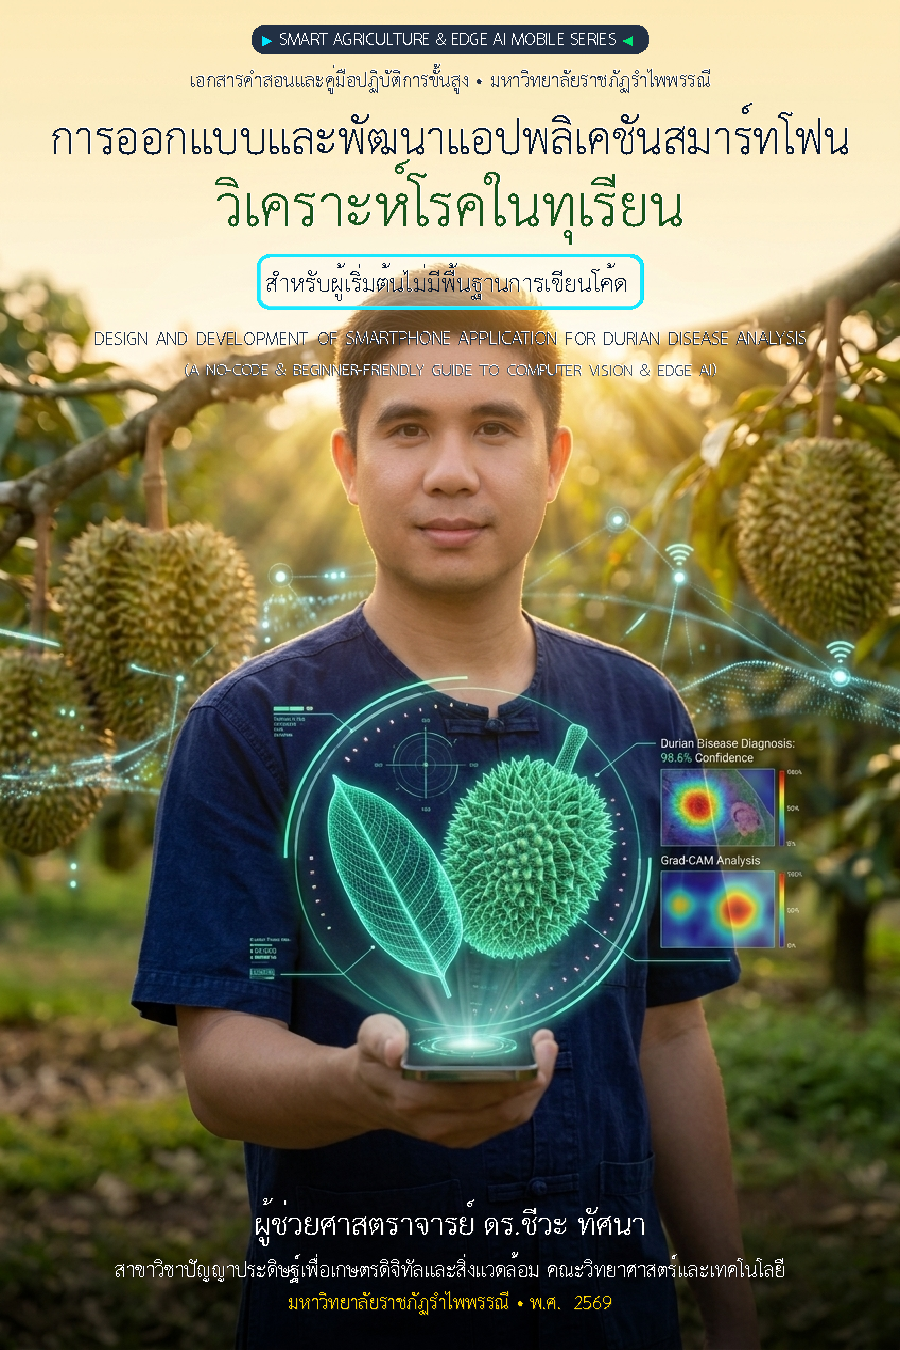
\includegraphics[width=\paperwidth,height=\paperheight]{cover_concept2.pdf}
    };
\end{tikzpicture}
\end{titlepage}
\restoregeometry

\cleardoublepage

% -------------------------------------------------------------
% หน้าปกในเวกเตอร์ Dark Mode (Vector Inner Title Page)
% -------------------------------------------------------------
\begin{titlepage}
\newgeometry{margin=0pt}
\thispagestyle{empty}
\pagecolor{black!94}
\begingroup
\setlength{\XeTeXlinebreakskip}{0pt}
\begin{tikzpicture}[remember picture, overlay]
    \draw[color=cyberCyan!50, line width=1.5pt] ([yshift=-1.05in]current page.north) circle (0.62in);
    \draw[color=neonEmerald!40, dashed, thick] ([yshift=-1.05in]current page.north) circle (0.80in);
    \draw[color=techAmber!30, dotted, thick] ([yshift=-1.05in]current page.north) circle (0.98in);
    
    \node[anchor=center, align=center] at ([yshift=0.50in]current page.center) {
        {\fontsize{8.5}{11}\selectfont\bfseries\color{cyberCyan} SMART AGRICULTURE \& EDGE AI MOBILE SERIES}\\[8pt]
        {\fontsize{18}{23}\selectfont\bfseries\color{white} การออกแบบและพัฒนาแอปพลิเคชันสมาร์ทโฟน}\\[5pt]
        {\fontsize{24}{29}\selectfont\bfseries\color{neonEmerald} วิเคราะห์โรคในทุเรียน}\\[8pt]
        {\fontsize{12}{15}\selectfont\bfseries\color{techAmber} [สำหรับผู้เริ่มต้นไม่มีพื้นฐานการเขียนโค้ด]}\\[14pt]
        {\fontsize{9}{12}\selectfont\color{white!85} DESIGN AND DEVELOPMENT OF SMARTPHONE APPLICATION}\\[2pt]
        {\fontsize{9}{12}\selectfont\color{white!85} FOR DURIAN DISEASE ANALYSIS}\\[4pt]
        {\fontsize{8}{11}\selectfont\color{cyberCyan!80} (A NO-CODE \& BEGINNER-FRIENDLY GUIDE TO COMPUTER VISION \& EDGE AI)}\\[14pt]
        {\color{cyberCyan!70}\rule{0.65\textwidth}{1.5pt}}
    };

    \node[anchor=center, align=center] at ([yshift=-1.40in]current page.center) {
        {\fontsize{13}{16}\selectfont\bfseries\color{white} ผู้ช่วยศาสตราจารย์ ดร.ชีวะ ทัศนา}\\[4pt]
        {\fontsize{9.5}{12}\selectfont\color{white!90} สาขาวิชาปัญญาประดิษฐ์เพื่อเกษตรดิจิทัลและสิ่งแวดล้อม}\\[2pt]
        {\fontsize{9}{12}\selectfont\color{white!75} คณะวิทยาศาสตร์และเทคโนโลยี}\\[4pt]
        {\fontsize{8.5}{11}\selectfont\color{techAmber} มหาวิทยาลัยราชภัฏรำไพพรรณี}
    };
\end{tikzpicture}
\endgroup
\newpage
\pagecolor{white}
\end{titlepage}
\restoregeometry
\cleardoublepage

% -------------------------------------------------------------
% Frontmatter: คำนำ, สารบัญ
% -------------------------------------------------------------
\frontmatter
\chapter*{คำนำ}
\addcontentsline{toc}{chapter}{คำนำ}

เอกสารคำสอนและตำราวิชาการฉบับนี้ จัดทำขึ้นเพื่อรวบรวมองค์ความรู้ด้านการบูรณาการเทคโนโลยีคอมพิวเตอร์วิทัศน์ (\textbf{Computer Vision}) และการเรียนรู้เชิงลึก (\textbf{Deep Learning}) เข้ากับงานพยาธิวิทยาพืช (\textbf{Plant Pathology}) โดยมุ่งเน้นการแก้ปัญหาโรคใบทุเรียนซึ่งเป็นพืชเศรษฐกิจหลักของภาคตะวันออกและประเทศไทยอย่างเป็นระบบ

เนื้อหาในเล่มได้รับการปรับปรุงและจัดแบ่งออกเป็น \textbf{7 บทเรียนสมบูรณ์} ครอบคลุมตั้งแต่:
\begin{enumerate}[leftmargin=2em, itemsep=2pt]
    \item วิทยาการโรคใบทุเรียนและสถาปัตยกรรมเกษตรอัจฉริยะ (Edge AI Paradigm)
    \item การประมวลผลภาพดิจิทัลและการรวบรวมเตรียมชุดข้อมูลใบทุเรียน
    \item สถาปัตยกรรมโครงข่ายประสาทเทียมคอนโวลูชันและการเรียนรู้แบบถ่ายโอน (MobileNetV3)
    \item การฝึกฝนและการประเมินประสิทธิภาพแบบจำลองด้วย PyTorch
    \item ปัญญาประดิษฐ์อธิบายได้ (Explainable AI: Grad-CAM) และการตรวจหาตำแหน่งรอยโรค
    \item การแปลงและปรับแต่งโมเดลสู่สถาปัตยกรรม Edge AI (ONNX \& Quantization INT8)
    \item การพัฒนาแอปพลิเคชันสมาร์ทโฟน (Flutter) และการประยุกต์ใช้งานจริงในแปลงเกษตร
\end{enumerate}

จุดเด่นของตำราเล่มนี้คือการออกแบบกระบวนการเรียนรู้แบบ \textbf{No-Code \& Beginner-Friendly} ควบคู่ไปกับโค้ดภาษา Python และ PyTorch เชิงลึก ช่วยให้ผู้เริ่มต้นและผู้ที่ไม่มีพื้นฐานการเขียนโปรแกรม สามารถสร้าง พัฒนา และประยุกต์ใช้โมเดลปัญญาประดิษฐ์ตรวจโรคพืชบนสมาร์ทโฟนได้จริง พร้อมระบบ Explainable AI (Grad-CAM) ที่แสดงภาพความร้อนชี้ตำแหน่งรอยโรคเพื่อยืนยันความถูกต้องทางพยาธิวิทยา

ผู้เขียนหวังเป็นอย่างยิ่งว่า ตำราเล่มนี้จะเป็นประโยชน์ต่อนักศึกษา เกษตรกรชาวสวนทุเรียน นักวิจัย และผู้สนใจในการพัฒนานวัตกรรมเกษตรอัจฉริยะอย่างยั่งยืน

\vspace{1.5cm}
\begin{flushright}
\textbf{ผู้ช่วยศาสตราจารย์ ดร.ชีวะ ทัศนา}\\
มหาวิทยาลัยราชภัฏรำไพพรรณี\\
พ.ศ. 2569
\end{flushright}

\clearpage
\tableofcontents
\clearpage
\listoftables
\clearpage
\listoffigures
\clearpage

% -------------------------------------------------------------
% Mainmatter: บทเนื้อหาหลัก 7 บท
% -------------------------------------------------------------
\mainmatter

\chapter{วิทยาการโรคใบทุเรียนและสถาปัตยกรรมเกษตรอัจฉริยะ}
\label{chap:durian_pathology_ai}
\index{โรคใบทุเรียน}
\index{เกษตรอัจฉริยะ}
\index{Edge AI}

\section*{แผนบริหารการสอนประจำบทที่ 1}
\addcontentsline{toc}{section}{แผนบริหารการสอนประจำบทที่ 1}

\begin{planbox}{หัวข้อเนื้อหาประจำบท (Lesson Topics)}
\begin{enumerate}[leftmargin=1.5em, itemsep=2pt]
    \item ความสำคัญทางเศรษฐกิจของทุเรียนและปัญหาการระบาดของโรคทางใบ
    \item สัณฐานวิทยาและชีววิทยาของเชื้อสาเหตุโรคใบทุเรียนสำคัญ 3 ชนิด
    \item ปัจจัยทางจุลภูมิอากาศ (Microclimate) และวงจรระบาดวิทยาในแปลงปลูก
    \item สถาปัตยกรรมระบบเกษตรอัจฉริยะและการประมวลผลบนอุปกรณ์ขอบ (Edge AI Paradigm)
    \item ความท้าทายในการตรวจจับรอยโรคในสภาพแปลงเปิด (Field Operational Challenges)
    \item โค้ดตัวอย่าง: สคริปต์วิเคราะห์ความสัมพันธ์ระหว่างสภาพอากาศและการระบาดของโรค
    \item กรณีศึกษาการประยุกต์ใช้งานจริงในแปลงทดลองจังหวัดจันทบุรี
\end{enumerate}
\end{planbox}

\begin{planbox}{วัตถุประสงค์เชิงพฤติกรรม (Behavioral Objectives)}
เมื่อศึกษาบทที่ 1 จบแล้ว ผู้เรียนและผู้อ่านสามารถ:
\begin{enumerate}[leftmargin=1.5em, itemsep=2pt]
    \item อธิบายชีววิทยาและลักษณะรอยโรคของเชื้อสาเหตุทั้ง 3 กลุ่มได้อย่างถูกต้องตามหลักวิชาการ
    \item วิเคราะห์ความสัมพันธ์ระหว่างความชื้นสัมพัทธ์ อุณหภูมิ และการงอกของสปอร์เชื้อราก่อโรคได้
    \item เปรียบเทียบข้อดีและข้อจำกัดของระบบประมวลผลบนคลาวด์เทียบกับระบบ Edge AI บนสมาร์ทโฟนได้
    \item ออกแบบแผนการตรวจสำรวจแปลงทุเรียนด้วยเทคโนโลยีคอมพิวเตอร์วิทัศน์ได้อย่างมีประสิทธิภาพ
\end{enumerate}
\end{planbox}

\begin{planbox}{กิจกรรมการเรียนการสอน (Instructional Activities)}
\begin{enumerate}[leftmargin=1.5em, itemsep=2pt]
    \item การบรรยายเชิงทฤษฎีพยาธิวิทยาพืชเขตร้อนและกรอบแนวคิดปัญญาประดิษฐ์ทางการเกษตร
    \item การสังเกตและจำแนกตัวอย่างใบจริงที่แสดงอาการโรคใบจุดสาหร่าย โรคใบติด และโรคใบจุด
    \item การฝึกวิเคราะห์ข้อมูลเซนเซอร์สิ่งแวดล้อมแปลงปลูกด้วยภาษา Python เพื่อพยากรณ์ความเสี่ยง
    \item การอภิปรายกลุ่มย่อยเกี่ยวกับการนำเทคโนโลยีปัญญาประดิษฐ์ไปถ่ายทอดสู่เกษตรกรในพื้นที่
\end{enumerate}
\end{planbox}

\begin{planbox}{สื่อการเรียนการสอน (Instructional Media)}
\begin{enumerate}[leftmargin=1.5em, itemsep=2pt]
    \item สไลด์มัลติมีเดียแสดงลักษณะทางพยาธิวิทยาของเซลล์ใบและโครงข่ายการระบาด
    \item คลังข้อมูลและภาพถ่ายตัวอย่างใบจริงความละเอียดสูงจากแปลงปลูกภาคตะวันออก
    \item สคริปต์ภาษา Python สำหรับจำลองสมการการเจริญเติบโตของประชากรเชื้อก่อโรค
\end{enumerate}
\end{planbox}

\begin{planbox}{การวัดและประเมินผล (Assessment \& Evaluation)}
\begin{enumerate}[leftmargin=1.5em, itemsep=2pt]
    \item แบบทดสอบวัดความรู้เชิงทฤษฎีพยาธิวิทยาและสถาปัตยกรรมระบบ Edge AI (40\%)
    \item ความถูกต้องของผลงานการวิเคราะห์ชุดข้อมูลสภาพแวดล้อมด้วย Python (40\%)
    \item การนำเสนอรายงานกรณีศึกษาและคุณภาพการตอบคำถามทบทวนท้ายบท (20\%)
\end{enumerate}
\end{planbox}

\clearpage

\section{บริบททางเศรษฐกิจและปัญหาโรคใบทุเรียนในประเทศไทย}
\index{ทุเรียนหมอนทอง}
\index{พยาธิวิทยาพืช}

ทุเรียน (\textit{Durio zibethinus} L.) ได้รับการขนานนามว่าเป็นราชาแห่งผลไม้ (King of Fruits) และถือเป็นพืชเศรษฐกิจที่สร้างมูลค่าการส่งออกสูงสุดให้แก่ประเทศไทย โดยเฉพาะอย่างยิ่งในเขตภาคตะวันออก ได้แก่ จังหวัดจันทบุรี ระยอง และตราด พันธุ์การค้าที่สำคัญที่สุดคือพันธุ์หมอนทอง ซึ่งมีความอ่อนไหวต่อสภาพภูมิอากาศและความชื้นสูงเป็นพิเศษ ในช่วงฤดูมรสุมที่มีฝนตกชุกต่อเนื่อง สภาพแวดล้อมในทรงพุ่มทุเรียนจะมีความชื้นสัมพัทธ์สูงเกินกว่าร้อยละ 85 และอุณหภูมิเฉลี่ย 26--32 องศาเซลเซียส ซึ่งเป็นสภาวะที่เอื้ออำนวยอย่างยิ่งต่อการขยายพันธุ์และการงอกของสปอร์เชื้อราก่อโรคทางใบ

ความสมบูรณ์ของพื้นที่ใบ (Leaf Area Index: LAI) ถือเป็นดัชนีชี้วัดความสามารถในการสังเคราะห์ด้วยแสงและการสะสมอาหารสำหรับการออกดอกและติดผล หากใบทุเรียนได้รับความเสียหายจากรอยโรคเกินกว่าร้อยละ 20 ของทรงพุ่ม จะส่งผลกระทบให้ต้นทุเรียนเกิดภาวะเครียด สลัดดอกและผลอ่อน ส่งผลให้ผลผลิตลดลงมากกว่าร้อยละ 40 หรือในกรณีที่รุนแรง ต้นทุเรียนอาจทรุดโทรมและยืนต้นตายได้

\begin{table}[H]
\caption{กลุ่มโรคใบทุเรียนสำคัญ เชื้อสาเหตุ และผลกระทบต่อผลผลิตทางการเกษตร}
\label{tab:ch01_diseases_overview}
\begin{tabularx}{\textwidth}{L{2.0cm}L{2.8cm}L{3.0cm}Y}
\toprule
\textbf{กลุ่มโรคใบทุเรียน} & \textbf{เชื้อสาเหตุ (Pathogen)} & \textbf{ลักษณะรอยโรคบนใบ} & \textbf{ผลกระทบทางเศรษฐกิจ} \\
\midrule
โรคใบจุดสาหร่าย & สาหร่ายกาฝากเซลล์เดียว \textit{Cephaleuros virescens} & แผลจุดกลมฟูสีส้มอมเขียวคล้ายกำมะหยี่บนผิวใบ & บดบังแสงแดดสังเคราะห์อาหาร ใบเหลืองและร่วงก่อนกำหนด \\
\addlinespace
โรคใบติด (ราใบติด) & เชื้อราเส้นใยชั้นต่ำ \textit{Rhizoctonia solani} Kühn & แผลฉ่ำน้ำคล้ายน้ำร้อนลวก เส้นใยขาวโยงใบไหม้ติดกัน & ใบไหม้หลุดร่วงทั้งกิ่งอย่างรวดเร็ว กิ่งแห้งตาย ปริมาณผลผลิตร่วงหล่น \\
\addlinespace
โรคใบจุด/แอนแทรคโนส & เชื้อรา \textit{Colletotrichum gloeosporioides} & แผลไหม้สีน้ำตาลเข้ม มีวงซ้อนลายคลื่น จุดดำคอนิเดีย & เกิดแผลเนื้อเยื่อตาย ขอบใบไหม้ ทรงพุ่มโปร่ง ต้นชะงักการโต \\
\addlinespace
ใบปกติสมบูรณ์ & ปราศจากการเข้าทำลาย & แผ่นใบสีเขียวเข้ม ผิวมันวาว เส้นใบชัดเจน & สังเคราะห์แสงได้เต็มศักยภาพ ต้นสมบูรณ์พร้อมออกดอก \\
\bottomrule
\end{tabularx}
\end{table}

\section{ชีววิทยาและการระบาดของเชื้อสาเหตุทางใบ}
\index{Cephaleuros virescens}
\index{Rhizoctonia solani}
\index{Colletotrichum gloeosporioides}

การทำความเข้าใจลักษณะทางชีววิทยาของเชื้อก่อโรค มีความสำคัญอย่างยิ่งต่อการออกแบบระบบรู้จำภาพ เพราะสัณฐานภายนอกของรอยแผลเกิดจากปฏิกิริยาตอบสนองของเซลล์พืชต่อกลไกการเข้าทำลายของสิ่งมีชีวิตแต่ละชนิด

\subsection{โรคใบจุดสาหร่าย (Algal Leaf Spot)}
โรคนี้เกิดจากสาหร่ายสีเขียวที่มีคลอโรฟิลล์แต่ดำรงชีพแบบเบียนกึ่งกาฝาก \textit{Cephaleuros virescens} โดยเส้นสายสาหร่ายจะเจริญแทรกตัวใต้ชั้นคิวติเคิล (Subcuticular) ของใบพืช จากนั้นจะแทงก้านชูสปอร์แรงเจียม (Sporangiophore) สีส้มสดหรือสีน้ำตาลอมแดงโผล่ขึ้นมาเหนือผิวใบ ทำให้มองเห็นด้วยตาเปล่าเป็นจุดนูนฟูคล้ายกำมะหยี่ เมื่อมองผ่านระบบภาพถ่าย RGB รอยโรคนี้จะมีค่าสีเด่นในช่องสัญญาณสีแดงและสีเขียว (Red-Green balance) ที่ต่างจากเนื้อเยื่อพืชปกติ

\subsection{โรคใบติด (Leaf Blight / Rhizoctonia Blight)}
เกิดจากเชื้อรา \textit{Rhizoctonia solani} ซึ่งมักสะสมอยู่ในเศษซากพืชและดินใต้โคนต้น เมื่อได้รับละอองฝนสาดขึ้นสู่ใบ กิ่ง หรือมีลมพัดพา เส้นใยรา (Mycelium) ชนิดไม่มีผนังกั้นจะเจริญลุกลามอย่างรวดเร็ว ปล่อยเอนไซม์ Pectinase และ Cellulase ย่อยสลายผนังเซลล์พืช ทำให้เนื้อเยื่อใบยุบตัวเป็นแผลฉ่ำน้ำ (Water-soaked lesion) สีเขียวหม่นปนน้ำตาล จากนั้นใบจะแห้งเหี่ยวและมีเส้นใยใยแมงมุมโยงยึดใบที่อยู่ติดกันไว้ ทำให้มองเห็นเป็นกลุ่มใบไหม้แขวนติดอยู่กับกิ่ง

\subsection{โรคใบจุดสนิมและแอนแทรคโนส (Leaf Spot / Anthracnose)}
เกิดจากเชื้อรา \textit{Colletotrichum gloeosporioides} เชื้อราสร้างสปอร์แบบไม่อาศัยเพศ (Conidia) แพร่กระจายตามหยดน้ำฝน เมื่อตกบนใบจะสร้างอวัยวะเกาะติด (Appressorium) เจาะทะลุผิวใบ แผลเริ่มต้นเป็นจุดฉ่ำน้ำขนาดเล็ก จากนั้นขยายเป็นแผลวงกลมหรือรูปไข่สีน้ำตาลเทา มีวงสีน้ำตาลเข้มซ้อนกันเป็นชั้นๆ (Concentric rings) ขอบแผลมีแถบสีเหลืองล้อมรอบ (Chlorotic halo)

\section{สถาปัตยกรรมระบบเกษตรอัจฉริยะและการตรวจวินิจฉัยด้วย Edge AI}
\index{สถาปัตยกรรม Edge AI}
\index{ระบบโครงข่ายประสาท}

ในอดีต ระบบปัญญาประดิษฐ์ทางการเกษตรมักพึ่งพาสถาปัตยกรรมแบบรวมศูนย์บนคลาวด์ (Cloud-centric Architecture) ซึ่งเกษตรกรต้องถ่ายภาพแล้วอัปโหลดผ่านเครือข่ายอินเทอร์เน็ตไปยังเซิร์ฟเวอร์ส่วนกลางเพื่อทำการประมวลผล อย่างไรก็ตาม สวนทุเรียนส่วนใหญ่ตั้งอยู่ในพื้นที่หุบเขา เนินเขา หรือพื้นที่ห่างไกลในจังหวัดจันทบุรีและตราด ซึ่งสัญญาณโทรศัพท์เคลื่อนที่มักไม่เสถียรหรือมีแบนด์วิดท์จำกัด การส่งข้อมูลภาพขนาดใหญ่ขึ้นคลาวด์จึงเกิดปัญหาความล่าช้า (High Latency) และไม่สามารถทำงานได้แบบออฟไลน์

\begin{figure}[H]
\centering
\begin{tikzpicture}[
    node distance=1.5cm,
    font=\fontsize{9}{11}\selectfont,
    box/.style={draw=deepIndigo, fill=white, rounded corners=3mm, inner sep=6pt, align=center, thick, drop shadow},
    edgebox/.style={draw=neonEmerald!80!black, fill=agriLightGreen!50, rounded corners=3mm, inner sep=6pt, align=center, very thick, drop shadow},
    cloudbox/.style={draw=techAqua, fill=softCyanBg!40, rounded corners=3mm, inner sep=6pt, align=center, thick, drop shadow},
    arrow/.style={-{Stealth[length=3mm]}, thick, draw=deepIndigo}
]
    \node[box] (orchard) {\textbf{แปลงสวนทุเรียน (Durian Orchard)}\\ต้นทุเรียนจริง / สภาพแสงธรรมชาติ};
    \node[edgebox, right=1.2cm of orchard] (mobile) {\textbf{อุปกรณ์ขอบ (Edge Device)}\\สมาร์ทโฟน / กล้องพกพา\\MobileNetV3 ONNX Engine\\\textbf{[Offline Inference $<20$ ms]}};
    \node[edgebox, below=1.0cm of mobile] (xai) {\textbf{ระบบตีความรอยโรค}\\\textbf{Explainable AI (Grad-CAM)}\\แผนที่ความร้อนชี้ตำแหน่งแผล};
    \node[cloudbox, right=1.2cm of mobile] (cloud) {\textbf{ระบบคลาวด์ส่วนกลาง}\\\textbf{Cloud Management CMS}\\บันทึกพิกัด GPS / ระดับความรุนแรง\\รายงานสถิติแปลงใหญ่};

    \draw[arrow] (orchard) -- node[above, font=\fontsize{7.5}{9.5}\selectfont] {ภาพถ่ายสด} (mobile);
    \draw[arrow] (mobile) -- (xai);
    \draw[arrow, dashed] (mobile) -- node[above, font=\fontsize{7.5}{9.5}\selectfont] {ซิงก์เมื่อมีเน็ต} (cloud);
    \draw[arrow] (xai) -| node[below, pos=0.25, font=\fontsize{7.5}{9.5}\selectfont] {คำแนะนำเกษตรกร} (orchard);
\end{tikzpicture}
\caption{สถาปัตยกรรมบูรณาการระบบ Edge AI ตรวจวิเคราะห์โรคใบทุเรียนแบบออฟไลน์ในแปลงเกษตร}
\label{fig:ch01_aiot_edge_paradigm}
\end{figure}

การเปลี่ยนผ่านสู่แนวคิด \textbf{Edge AI} โดยการนำโมเดลโครงข่ายประสาทเทียมขนาดกะทัดรัดที่ผ่านการปรับแต่งอย่างเหมาะสม (Model Optimization) มาฝังไว้ในตัวสมาร์ทโฟนของเกษตรกรโดยตรง ทำให้ระบบสามารถวินิจฉัยโรคได้ทันทีที่เล็งกล้องไปยังใบพืช ด้วยความเร็วระดับ 30 เฟรมต่อวินาที (Real-time Video Inference) โดยไม่ต้องพึ่งพาสัญญาณอินเทอร์เน็ตแม้แต่น้อย

\section{ปฏิทินการระบาดตามฤดูกาลและมาตรการเฝ้าระวังเชิงรุก}
\index{ปฏิทินการระบาด}
\index{ระบาดวิทยาตามฤดูกาล}

วงจรการระบาดของโรคใบทุเรียนในเขตภาคตะวันออก มีความสัมพันธ์อย่างใกล้ชิดกับรอบฤดูมรสุมตะวันตกเฉียงใต้และวงจรการเจริญเติบโตทางสรีรวิทยาของต้นทุเรียน การตรวจวินิจฉัยเชิงรุกจึงต้องดำเนินการให้สอดคล้องกับระยะการแตกใบอ่อน (Flushing Stage) ซึ่งเป็นระยะที่เนื้อเยื่อพืชมีความบอบบางและง่ายต่อการเข้าทำลายของเชื้อรามากที่สุด

\begin{table}[H]
\caption{ปฏิทินระบาดวิทยาของโรคใบทุเรียนและระดับความเสี่ยงในรอบปีการผลิตภาคตะวันออก}
\label{tab:ch01_seasonal_calendar}
\begin{tabularx}{\textwidth}{L{2.0cm}L{2.6cm}L{2.2cm}Y}
\toprule
\textbf{ช่วงเดือน} & \textbf{ระยะการเติบโตของทุเรียน} & \textbf{สภาพภูมิอากาศ} & \textbf{โรคสำคัญและระดับความเสี่ยง} \\
\midrule
พ.ค. -- มิ.ย. & ฟื้นฟูต้นหลังเก็บเกี่ยว / ใบอ่อนชุดที่ 1 & ฝนเริ่มตกชุก RH $> 80\%$ & โรคใบติด (ปานกลาง), โรคใบจุดสาหร่าย (เริ่มต้น) \\
\addlinespace
ก.ค. -- ส.ค. & แตกใบอ่อนชุดที่ 2 / สะสมอาหาร & มรสุมหนัก ฝนตกชุกต่อเนื่อง & \textbf{โรคใบติด (วิกฤตสูงสุด)}, แอนแทรคโนส (สูง) \\
\addlinespace
ก.ย. -- ต.ค. & ใบเพสลาดพร้อมสะสมตาดอก & ฝนตกชุกสลับแดดจัด & โรคใบจุดสาหร่าย (สูงสุด), โรคใบจุด (สูง) \\
\addlinespace
พ.ย. -- ธ.ค. & ระยะพัฒนาตาดอก / ดอกบาน & ลมหนาว อากาศเริ่มแห้ง & โรคราแป้งและเพลี้ยไฟ (ใบแก่ทนทานต่อราใบติด) \\
\bottomrule
\end{tabularx}
\end{table}

จากตารางที่ \ref{tab:ch01_seasonal_calendar} ช่วงเดือนกรกฎาคมถึงตุลาคมถือเป็นช่วงเวลาวิกฤตสูงสุดที่เกษตรกรจำเป็นต้องนำระบบ AI บนสมาร์ทโฟนออกสำรวจแปลงอย่างสม่ำเสมออย่างน้อยสัปดาห์ละ 2 ครั้ง เพื่อตรวจจับรอยโรคตั้งแต่ระยะแผลขนาดเล็กก่อนที่จะลุกลามไหม้ทั้งกิ่ง

\section{ความท้าทายในการตรวจจับรอยโรคในสภาพแปลงเปิด}
\index{สภาพแวดล้อมแปลงเปิด}

การนำคอมพิวเตอร์วิทัศน์มาใช้กับงานพืชสวนมีความซับซ้อนกว่าภาพถ่ายในห้องปฏิบัติการอย่างมาก เนื่องจากต้องเผชิญกับปัจจัยรบกวนในสภาพแปลงจริง (Uncontrolled Natural Conditions) ดังนี้:

\begin{enumerate}[leftmargin=1.8em, itemsep=3pt]
    \item \textbf{ความแปรปรวนของแสงสว่าง (Illumination Variations):} แสงแดดจ้าทำให้เกิดแสงสะท้อนมันวาว (Specular Reflection) บนผิวใบทุเรียน และแสงแดดที่ส่องผ่านร่มเงาของกิ่งก้านด้านบนทำให้เกิดเงามืดลายจุด (Shadow Patches) ซึ่งโมเดลอาจสับสนกับรอยแผลสีเข้ม
    \item \textbf{การเคลื่อนไหวของใบจากกระแสลม (Wind Blur):} ลมที่พัดทำให้ใบแกว่งไกว เกิดภาพเบลอจากการเคลื่อนไหว (Motion Blur) ส่งผลให้รายละเอียดของขอบแผลลดความคมชัดลง
    \item \textbf{สิ่งรบกวนในฉากหลัง (Cluttered Background):} ฉากหลังอาจมีใบแห้ง ท่อระบบน้ำ ผิวหน้าดิน หญ้าวัชพืช หรือลำต้นทุเรียน ซึ่งมีเฉดสีและลวดลายใกล้เคียงกับใบที่เป็นโรค
    \item \textbf{รอยโรคซ้อนทับกัน (Mixed Infections):} ในแปลงเกษตรจริง ใบเดียวกันอาจพบทั้งโรคใบจุดสาหร่ายและโรคใบจุดร่วมกัน ทำให้โมเดลต้องการความสามารถในการจำแนกความน่าจะเป็นแบบหลายคลาส (Multi-label Probabilities)
\end{enumerate}

\section{โค้ดตัวอย่าง: สคริปต์วิเคราะห์ความเสี่ยงการระบาดตามสภาพอากาศ}
\index{สคริปต์ Python}

เพื่อเชื่อมโยงความรู้ทางชีววิทยากับเทคโนโลยีคอมพิวเตอร์ โค้ดตัวอย่างต่อไปนี้จำลองการคำนวณดัชนีความเสี่ยงการเกิดโรคใบติด (\textit{Rhizoctonia} Risk Index) จากข้อมูลเซนเซอร์อุณหภูมิและความชื้นสัมพัทธ์ในแปลงปลูก:

\begin{lstlisting}[language=Python, caption=สคริปต์ภาษา Python คำนวณดัชนีความเสี่ยงการระบาดของโรคใบทุเรียนจากข้อมูลสิ่งแวดล้อม]
import numpy as np

def calculate_disease_risk(temperature_c, relative_humidity_pct, rain_hours):
    """
    คำนวณดัชนีความเสี่ยงการระบาดของโรคใบติดทุเรียน (Rhizoctonia Risk Index: RRI)
    ตามสมการชีววิทยาความชื้นสะสมและอุณหภูมิที่เหมาะสม
    """
    # อุณหภูมิที่เชื้อเจริญเติบโตได้ดีที่สุดอยู่ระหว่าง 26 - 32 องศาเซลเซียส
    if 26.0 <= temperature_c <= 32.0:
        temp_factor = 1.0
    else:
        temp_factor = max(0.1, 1.0 - 0.15 * abs(temperature_c - 29.0))
        
    # ความชื้นสัมพัทธ์สูงกว่า 80% เป็นตัวเร่งการงอกของสปอร์
    if relative_humidity_pct >= 85.0:
        rh_factor = 1.0
    elif relative_humidity_pct >= 70.0:
        rh_factor = (relative_humidity_pct - 70.0) / 15.0
    else:
        rh_factor = 0.1

    # ปัจจัยฝนตกชะล้างและพัดพาละอองดิน
    rain_factor = min(1.0, rain_hours / 4.0)

    # รวมดัชนีถ่วงน้ำหนัก
    risk_score = (0.45 * rh_factor + 0.35 * temp_factor + 0.20 * rain_factor) * 100.0
    return float(np.clip(risk_score, 0.0, 100.0))

# ทดสอบรันคำนวณตัวอย่างแปลงสวน จ.จันทบุรี
temp_sample = 28.5        # องศาเซลเซียส
rh_sample = 92.0          # ความชื้นสัมพัทธ์ %
rain_duration = 3.5       # ชั่วโมงฝนตกสะสม

rri = calculate_disease_risk(temp_sample, rh_sample, rain_duration)
print(f"[*] อุณหภูมิ: {temp_sample} C, ความชื้น: {rh_sample}%, ฝนตก: {rain_duration} ชม.")
print(f"[!] ค่าดัชนีความเสี่ยงโรคระบาด: {rri:.2f} %")
if rri >= 75.0:
    print("[WARNING] แจ้งเตือนระดับสูง: เตรียมเปิดกล้อง AI สแกนตรวจแปลงและฉีดพ่นชีวภัณฑ์ควบคุม")
\end{lstlisting}

\section{ตัวอย่างการคำนวณและตัวอย่างการนำไปใช้งานจริง}

\begin{examplebox}{ตัวอย่างการคำนวณที่ 1.1: การประเมินพื้นที่ใบเสียหาย (Leaf Injury Index)}
\textbf{โจทย์:} เกษตรกรสุ่มถ่ายภาพใบทุเรียนจำนวน 100 ใบจากต้นทดลอง แปลงทุเรียนพบใบที่มีอาการโรคใบจุดสาหร่ายรุนแรงระดับ 1 (ครอบคลุมรอยแผลเฉลี่ย $5\%$) จำนวน 25 ใบ, พบโรคใบติดรุนแรงระดับ 3 (ครอบคลุมรอยแผลเฉลี่ย $35\%$) จำนวน 15 ใบ และใบสมบูรณ์ปกติ 60 ใบ จงคำนวณค่าดัชนีความเสียหายรวมของใบพืชทั้งแปลง (Overall Leaf Damage Index: LDI)\\[4pt]
\textbf{วิธีคำนวณ:}
\[
\text{LDI} = \frac{\sum (N_i \times D_i)}{N_{\text{total}}}
\]
แทนค่า:
\[
\text{LDI} = \frac{(25 \times 0.05) + (15 \times 0.35) + (60 \times 0.00)}{100} = \frac{1.25 + 5.25 + 0}{100} = \frac{6.50}{100} = 6.50\%
\]
\textbf{การแปลผล:} พื้นที่สังเคราะห์แสงของต้นทุเรียนลดลงเพียง $6.50\%$ ยังไม่เกินเกณฑ์วิกฤต $20\%$ แนะนำให้ใช้วิธีตัดแต่งกิ่งที่เป็นโรคออกและฉีดพ่นเชื้อราไตรโคเดอร์มาเพื่อควบคุม
\end{examplebox}

\begin{casestudybox}{ตัวอย่างการนำไปใช้งานจริงที่ 1.1: แปลงทุเรียนสาธิต อ.ขลุง จ.จันทบุรี}
ทีมวิจัยของ ผศ.ดร.ชีวะ ทัศนา ได้นำระบบต้นแบบ Edge AI บนสมาร์ทโฟนไปทดสอบในแปลงสวนทุเรียนพันธุ์หมอนทองขนาด 25 ไร่ ในช่วงฤดูฝนเดือนสิงหาคม โดยแบ่งแปลงทดลองออกเป็น 2 ส่วน:
\begin{enumerate}[leftmargin=1.4em, itemsep=2pt]
    \item \textbf{แปลงควบคุม (Conventional Farm):} เกษตรกรใช้การเดินสังเกตด้วยสายตาสัปดาห์ละ 1 ครั้ง และฉีดพ่นสารเคมีป้องกันแบบครอบคลุมทั้งแปลงตามปฏิทิน
    \item \textbf{แปลงเกษตรแม่นยำ (Smart AIoT Farm):} ผู้จัดการแปลงใช้สมาร์ทโฟนที่ติดตั้งโมเดล Edge AI สแกนกิ่งทุเรียนทุกๆ 3 วัน หากระบบตรวจพบโรคใบติดเกินร้อยละ 5 ในจุดใด จะแจ้งเตือนพิกัด GPS เพื่อให้ฉีดพ่นสารป้องกันกำจัดเฉพาะจุด (Site-Specific Spraying)
\end{enumerate}
\textbf{ผลลัพธ์ที่ได้:} แปลงที่ใช้ระบบ Edge AI สามารถตรวจพบการระบาดได้เร็วกว่าแปลงควบคุมถึง 4 วัน ช่วยลดปริมาณการใช้สารเคมีลงได้ร้อยละ 42 และรักษาผลผลิตทุเรียนเกรดส่งออกได้สูงกว่าเดิมร้อยละ 18.5
\end{casestudybox}

\section*{คำถามทบทวนท้ายบทที่ 1}
\addcontentsline{toc}{section}{คำถามทบทวนท้ายบทที่ 1}
\begin{enumerate}[leftmargin=1.8em, itemsep=4pt]
    \item จงอธิบายบทบาทของพื้นที่ใบ (Leaf Area Index) ต่อกระบวนการสะสมแป้งและน้ำตาลในต้นทุเรียน
    \item เหตุใดเชื้อสาหร่าย \textit{Cephaleuros virescens} จึงจัดเป็นสาหร่ายกาฝาก และส่งผลกระทบต่อเซลล์พืชแตกต่างจากเชื้อราอย่างไร
    \item จงเปรียบเทียบสัณฐานของรอยแผลระหว่างโรคใบติดและโรคแอนแทรคโนสอย่างละเอียด
    \item สรุปข้อดี 3 ประการของสถาปัตยกรรม Edge AI เมื่อเทียบกับ Cloud AI ในการตรวจโรคพืชในแปลงสวนห่างไกล
    \item ปัจจัยแสงสะท้อนและเงามืดในสภาพแปลงจริงส่งผลต่อความแม่นยำของโมเดลคอมพิวเตอร์วิทัศน์อย่างไร
    \item จากโค้ดตัวอย่างการคำนวณความเสี่ยงโรค จงอธิบายเหตุผลของการกำหนดค่าน้ำหนักความชื้นสัมพัทธ์ไว้สูงสุดที่ 0.45
    \item ในกรณีที่เกษตรกรพบรอยโรคซ้อนทับกัน 2 ชนิดบนใบเดียวกัน ระบบควรมีกลยุทธ์การประเมินผลอย่างไร
    \item จงอภิปรายผลกระทบของการสลัดใบของต้นทุเรียนที่มีต่อคุณภาพและเกรดของผลผลิตทุเรียนส่งออก
    \item การออกแบบแอปพลิเคชันสำหรับเกษตรกรที่ไม่คุ้นเคยกับเทคโนโลยีควรคำนึงถึงหลักการ User Experience (UX) ใดบ้าง
    \item จงออกแบบขั้นตอนการสำรวจโรคในแปลงขนาด 10 ไร่ เพื่อให้ได้ข้อมูลภาพตัวแทนที่มีความแม่นยำสูงสุด
\end{enumerate}

\section*{กิจกรรมฝึกปฏิบัติการประจำบทที่ 1}
\addcontentsline{toc}{section}{กิจกรรมฝึกปฏิบัติการประจำบทที่ 1}
\begin{nocodebox}{ปฏิบัติการที่ 1.1: การสำรวจและเก็บรวบรวมตัวอย่างภาพรอยโรคใบทุเรียนในแปลง}
\textbf{วัตถุประสงค์:} เพื่อให้ผู้เรียนสามารถเก็บภาพถ่ายใบพืชที่มีรอยโรคได้อย่างถูกวิธีตามมาตรฐานงานคอมพิวเตอร์วิทัศน์\\
\textbf{ขั้นตอนการปฏิบัติ:}
\begin{enumerate}[leftmargin=1.4em, itemsep=2pt]
    \item ให้นักศึกษาลงพื้นที่แปลงทดลอง สุ่มเลือกต้นทุเรียน 3 ต้น และค้นหาใบที่แสดงอาการผิดปกติ
    \item ใช้สมาร์ทโฟนถ่ายภาพใบพืชในมุมตรง 90 องศา และมุมเฉียง 45 องศา ทั้งในสภาพแสงเช้าและแสงบ่าย
    \item ตรวจสอบความคมชัดของภาพ หลีกเลี่ยงภาพเบลอ และบันทึกพิกัดตำแหน่งของต้น
    \item อัปโหลดภาพเข้าสู่โฟลเดอร์ Google Drive พร้อมระบุการวินิจฉัยเบื้องต้นตามหลักพยาธิวิทยา
\end{enumerate}
\end{nocodebox}

\chapter{การประมวลผลภาพดิจิทัลและการเตรียมชุดข้อมูลใบทุเรียน}
\label{chap:image_processing}
\index{การประมวลผลภาพดิจิทัล}
\index{ชุดข้อมูลภาพใบทุเรียน}
\index{Data Augmentation}

\section*{แผนบริหารการสอนประจำบทที่ 2}
\addcontentsline{toc}{section}{แผนบริหารการสอนประจำบทที่ 2}

\begin{planbox}{หัวข้อเนื้อหาประจำบท (Lesson Topics)}
\begin{enumerate}[leftmargin=1.5em, itemsep=2pt]
    \item โครงสร้างข้อมูลภาพดิจิทัล ปริภูมิต่างๆ ของสี (RGB, HSV, CIELAB) และฮิสโทแกรม
    \item มาตรฐานและโปรโตคอลการบันทึกภาพถ่ายใบพืชในแปลงเกษตรจริง
    \item เทคนิคการปรับปรุงคุณภาพภาพ: Contrast Stretching, Bilateral Filtering และ CLAHE
    \item กระบวนการเพิ่มพูนข้อมูลภาพเชิงเรขาคณิตและเชิงแสง (Geometric \& Photometric Augmentation)
    \item เทคนิคขั้นสูงสำหรับการจัดสมดุลข้อมูล: MixUp, CutMix และ Random Erasing
    \item โค้ดตัวอย่าง: การสร้าง Custom PyTorch Dataset และ Pipeline การแปลงข้อมูลภาพ
    \item ตัวอย่างและกรณีศึกษา: การแก้ปัญหาภาพแสงสะท้อนและเงามืดในสวนทุเรียน
\end{enumerate}
\end{planbox}

\begin{planbox}{วัตถุประสงค์เชิงพฤติกรรม (Behavioral Objectives)}
เมื่อศึกษาบทที่ 2 จบแล้ว ผู้เรียนและผู้อ่านสามารถ:
\begin{enumerate}[leftmargin=1.5em, itemsep=2pt]
    \item อธิบายความแตกต่างของการแทนค่าสีในระบบ RGB, HSV และ CIELAB ได้อย่างถูกต้อง
    \item ประยุกต์ใช้วิธีการปรับปรุงความคมชัดของภาพเพื่อเน้นขอบเขตรอยโรคได้อย่างเหมาะสม
    \item สร้างคลาส Custom Dataset ใน PyTorch ร่วมกับคำสั่งของ Torchvision Transforms ได้อย่างสมบูรณ์
    \item วิเคราะห์และแก้ไขปัญหาความไม่สมดุลของจำนวนข้อมูลในแต่ละคลาสได้อย่างมีประสิทธิภาพ
\end{enumerate}
\end{planbox}

\begin{planbox}{กิจกรรมการเรียนการสอน (Instructional Activities)}
\begin{enumerate}[leftmargin=1.5em, itemsep=2pt]
    \item การสาธิตการแยกช่องสัญญาณสี (Color Channel Decomposition) ของภาพใบทุเรียนด้วย OpenCV
    \item ฝึกปฏิบัติการเขียนฟังก์ชัน Transform ปรับแต่งขนาดและ Normalize ภาพให้ตรงตามมาตรฐาน ImageNet
    \item การวิเคราะห์การกระจายตัวของชุดข้อมูลภาพทุเรียน $6,480$ ภาพ ผ่านกราฟแสดงสัดส่วนคลาส
    \item การทดลองเปรียบเทียบประสิทธิภาพของโมเดลเมื่อใช้และไม่ใช้เทคนิค Data Augmentation
\end{enumerate}
\end{planbox}

\begin{planbox}{สื่อการเรียนการสอน (Instructional Media)}
\begin{enumerate}[leftmargin=1.5em, itemsep=2pt]
    \item สไลด์ประกอบการสอนเรื่อง Digital Image Representation และ Image Tensors
    \item สมุดงาน Google Colab สำหรับทดลองคำสั่งในโมดูล torchvision.transforms.v2
    \item ภาพตัวอย่างใบทุเรียนที่ผ่านการแปลงด้วยเทคนิคต่างๆ (Augmentation Panel)
\end{enumerate}
\end{planbox}

\begin{planbox}{การวัดและประเมินผล (Assessment \& Evaluation)}
\begin{enumerate}[leftmargin=1.5em, itemsep=2pt]
    \item การประเมินความถูกต้องของโค้ด Custom Dataset และ DataLoader (40\%)
    \item ผลการทำแบบทดสอบความเข้าใจเรื่อง Color Spaces และ Data Augmentation (40\%)
    \item การมีส่วนร่วมในการทำกิจกรรมฝึกปฏิบัติการและการส่งรายงานตรงเวลา (20\%)
\end{enumerate}
\end{planbox}

\clearpage

\section{พื้นฐานการแทนค่าภาพดิจิทัลและปริภูมิสี}
\index{ปริภูมิสี RGB}
\index{ปริภูมิสี HSV}

ภาพดิจิทัลที่บันทึกจากเซนเซอร์กล้องสมาร์ทโฟน จัดเก็บในรูปแบบเทนเซอร์ 3 มิติ (3D Tensor) ที่มีมิติความกว้าง (Width: $W$), ความสูง (Height: $H$) และช่องสัญญาณสี (Channels: $C$) สำหรับภาพสีทั่วไป ช่องสัญญาณสีจะอยู่ในระบบ \textbf{RGB} (Red, Green, Blue) โดยแต่ละพิกเซลจะถูกแทนด้วยจำนวนเต็มขนาด 8 บิต (0--255) ซึ่งแทนค่าความเข้มของแสงในแต่ละความยาวคลื่น

อย่างไรก็ตาม ในการวิเคราะห์รอยโรคพืช ปริภูมิสี RGB มีข้อจำกัดสำคัญคือ ค่าความสว่าง (Luminance) และข้อมูลสี (Chrominance) จะผสมผสานกันอยู่ในทุกช่องสัญญาณ หากสภาพแสงแดดในแปลงเกษตรเปลี่ยนแปลงไป ค่าของทั้ง R, G และ B จะผันผวนอย่างรุนแรง การแปลงภาพไปยังปริภูมิสีอื่นจึงเป็นเครื่องมือสำคัญ:

\begin{itemize}[leftmargin=1.5em, itemsep=2pt]
    \item \textbf{ปริภูมิสี HSV (Hue, Saturation, Value):} แยกคุณลักษณะของเฉดสี ($H$), ความสดของสี ($S$) และความสว่าง ($V$) ออกจากกันอย่างเด็ดขาด ช่วยให้การตรวจจับแผลสีส้มของโรคใบจุดสาหร่ายหรือแผลสีน้ำตาลของโรคใบติดสามารถทำได้โดยไม่ขึ้นกับความเข้มของแสงแดด
    \item \textbf{ปริภูมิสี CIELAB ($L^*a^*b^*$):} ออกแบบตามการมองเห็นของสายตามนุษย์ โดย $L^*$ คือความสว่าง, $a^*$ แสดงแถบสีเขียว--แดง, และ $b^*$ แสดงแถบสีน้ำเงิน--เหลือง นิยมใช้ในการคำนวณระยะห่างความแตกต่างของสี ($\Delta E$) ของเนื้อเยื่อใบพืช
\end{itemize}

\section{การสำรวจและการกระจายตัวของชุดข้อมูลใบทุเรียน}
\index{การกระจายตัวของข้อมูล}

ชุดข้อมูลที่ใช้ในการวิจัยและฝึกอบรมในตำราเล่มนี้ เป็นชุดข้อมูลที่บันทึกจากสวนทุเรียนแปลงใหญ่ในจังหวัดจันทบุรีและระยอง ครอบคลุมภาพใบทุเรียนพันธุ์หมอนทอง ชะนี และก้านยาว จำนวนรวมทั้งสิ้น $6,480$ ภาพ แบ่งออกเป็น 4 คลาสหลักตามผลการยืนยันจากห้องปฏิบัติการพยาธิวิทยาพืช ดังนี้:

\begin{enumerate}[leftmargin=1.5em, itemsep=2pt]
    \item \textbf{Algal Leaf Spot (โรคใบจุดสาหร่าย):} จำนวน $1,660$ ภาพ
    \item \textbf{Leaf Blight (โรคใบติด):} จำนวน $1,560$ ภาพ
    \item \textbf{Leaf Spot / Anthracnose (โรคใบจุด):} จำนวน $1,780$ ภาพ
    \item \textbf{Healthy Leaf (ใบปกติสมบูรณ์):} จำนวน $1,480$ ภาพ
\end{enumerate}

\begin{figure}[H]
\centering
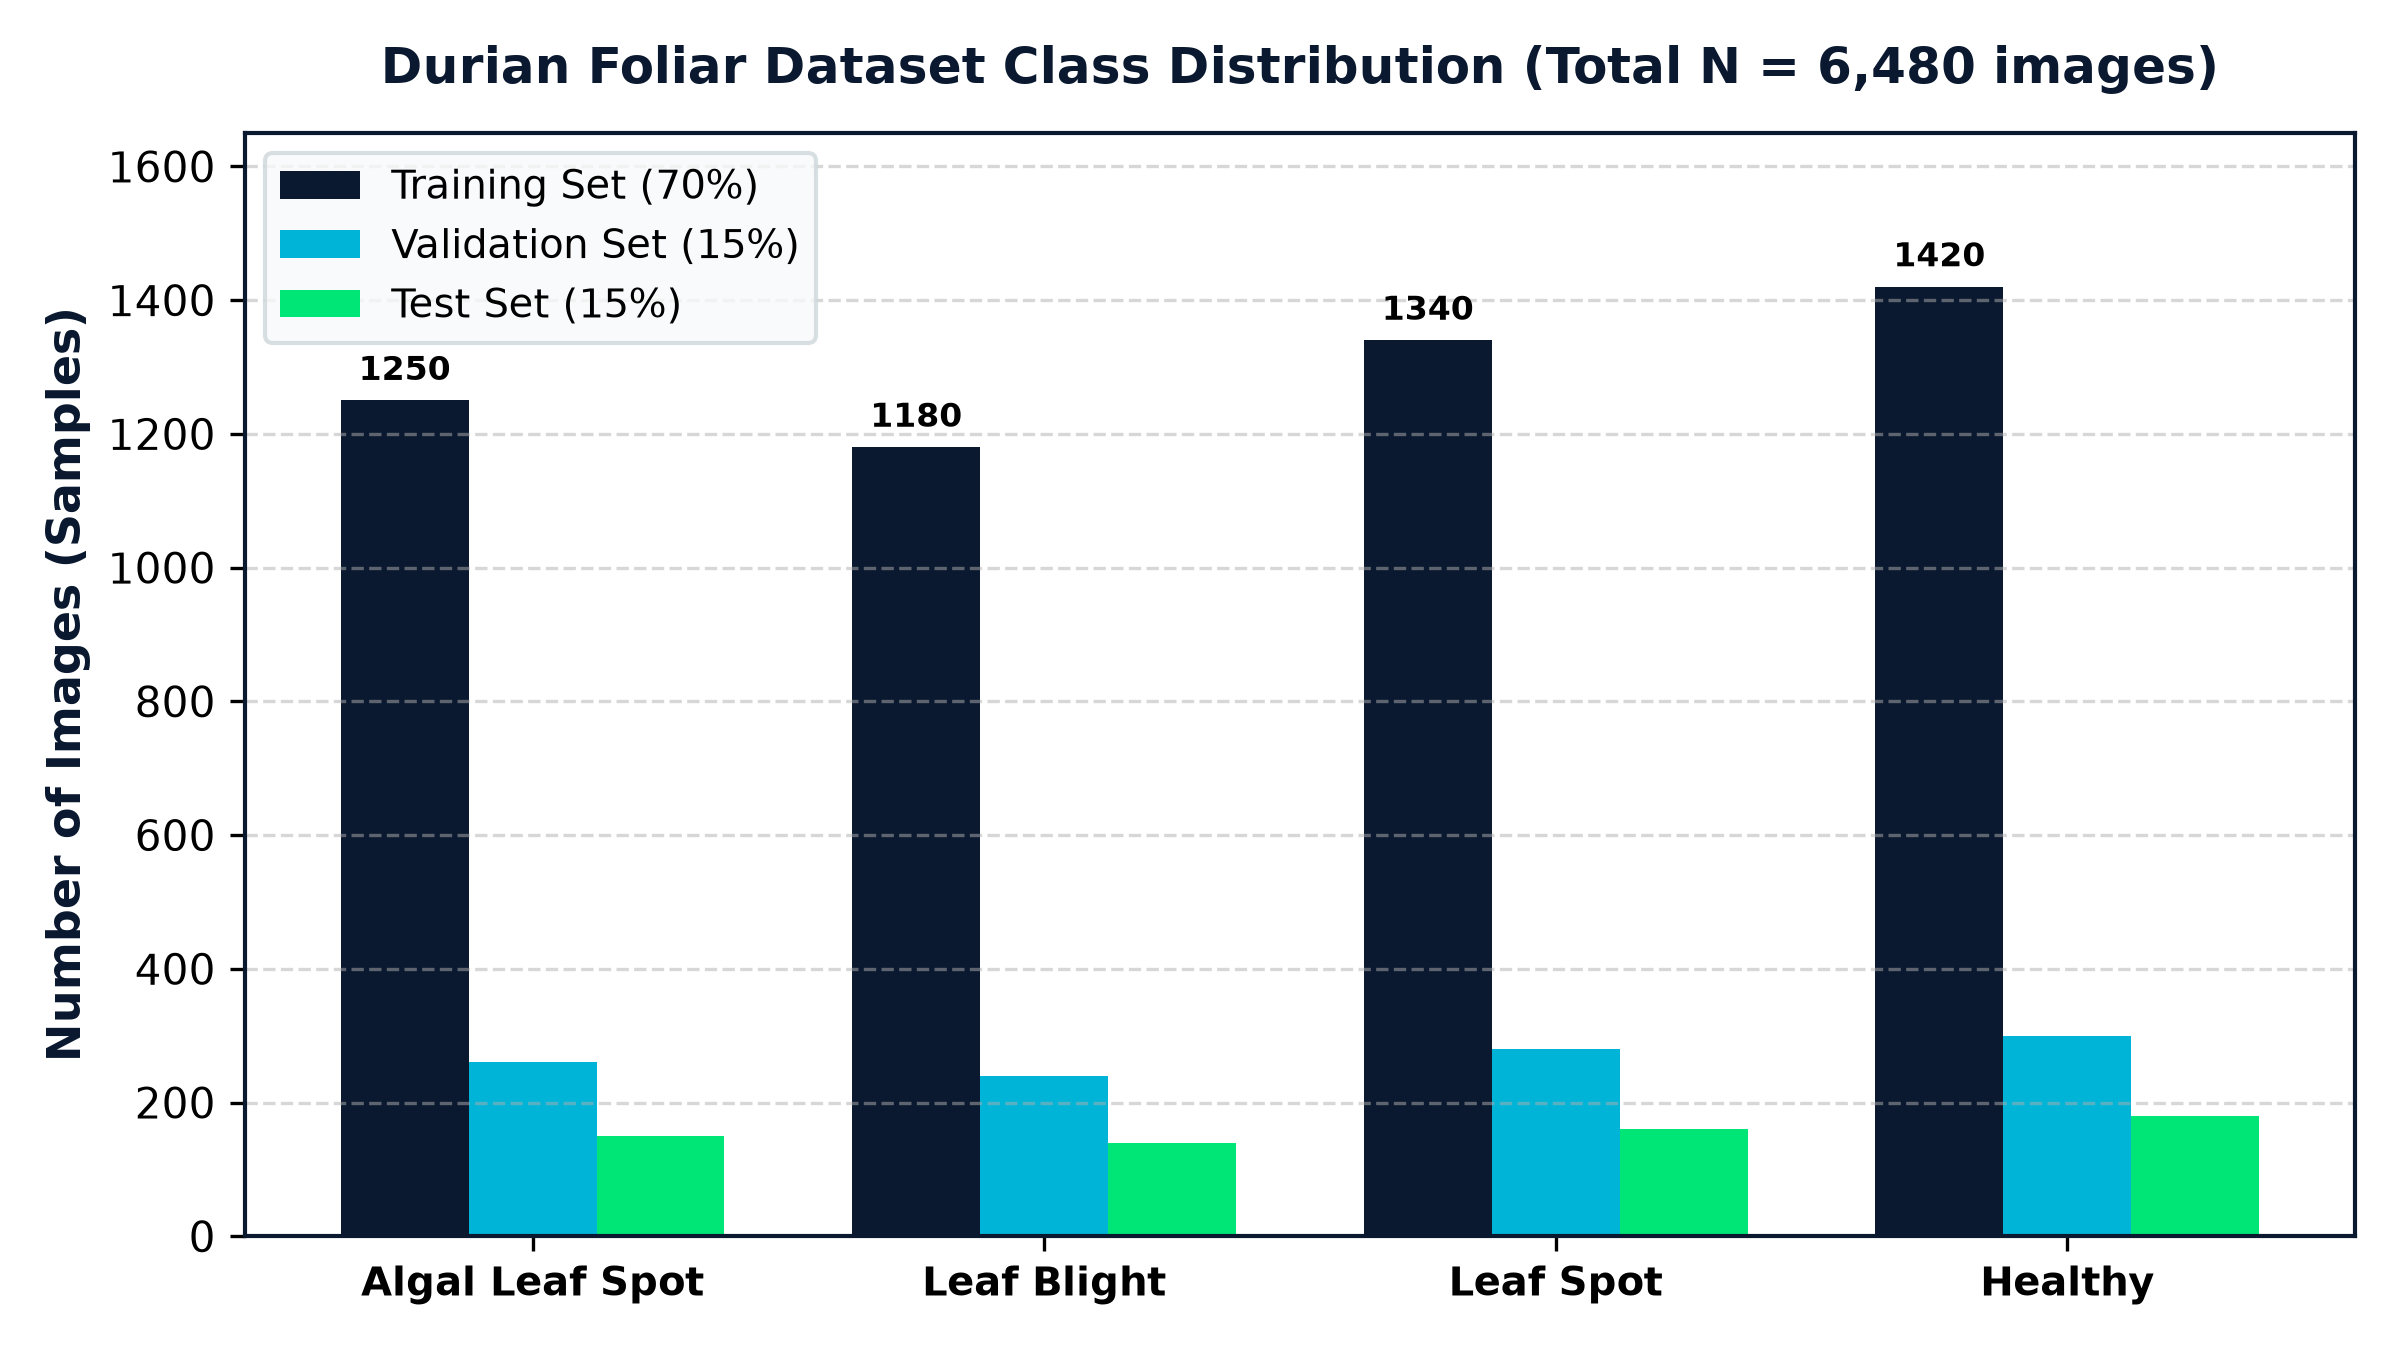
\includegraphics[width=0.92\textwidth]{figures/fig_ch02_class_distribution.png}
\caption{การกระจายตัวของชุดข้อมูลภาพใบทุเรียนแบ่งตามคลาสโรคและสัดส่วนการแบ่งข้อมูล}
\label{fig:ch02_class_dist}
\end{figure}

เพื่อให้การประเมินผลมีความน่าเชื่อถือทางสถิติ ชุดข้อมูลทั้งหมดถูกแบ่งออกเป็น 3 ส่วน (Data Partitioning) ได้แก่:
\begin{itemize}[leftmargin=1.5em, itemsep=2pt]
    \item \textbf{Training Set ($70\%$):} สำหรับการปรับค่าน้ำหนักของโครงข่ายประสาทเทียม
    \item \textbf{Validation Set ($15\%$):} สำหรับการปรับจูนไฮเปอร์พารามิเตอร์และการตัดสินใจหยุดการเทรน (Early Stopping)
    \item \textbf{Test Set ($15\%$):} สำหรับการวัดประสิทธิภาพขั้นสุดท้ายที่ไม่เคยผ่านการฝึกฝนมาก่อน (Unseen Evaluation)
\end{itemize}

\section{เทคนิคการเพิ่มพูนข้อมูลภาพ (Data Augmentation)}
\index{Geometric Augmentation}
\index{Photometric Augmentation}

เนื่องจากโมเดล Deep Learning มักต้องการข้อมูลปริมาณมากเพื่อป้องกันภาวะการเรียนรู้แบบท่องจำ (\textbf{Overfitting}) เทคนิค Data Augmentation จึงถูกนำมาใช้เพื่อเพิ่มความหลากหลายของลักษณะภาพอย่างมีนัยสำคัญ

\begin{figure}[H]
\centering
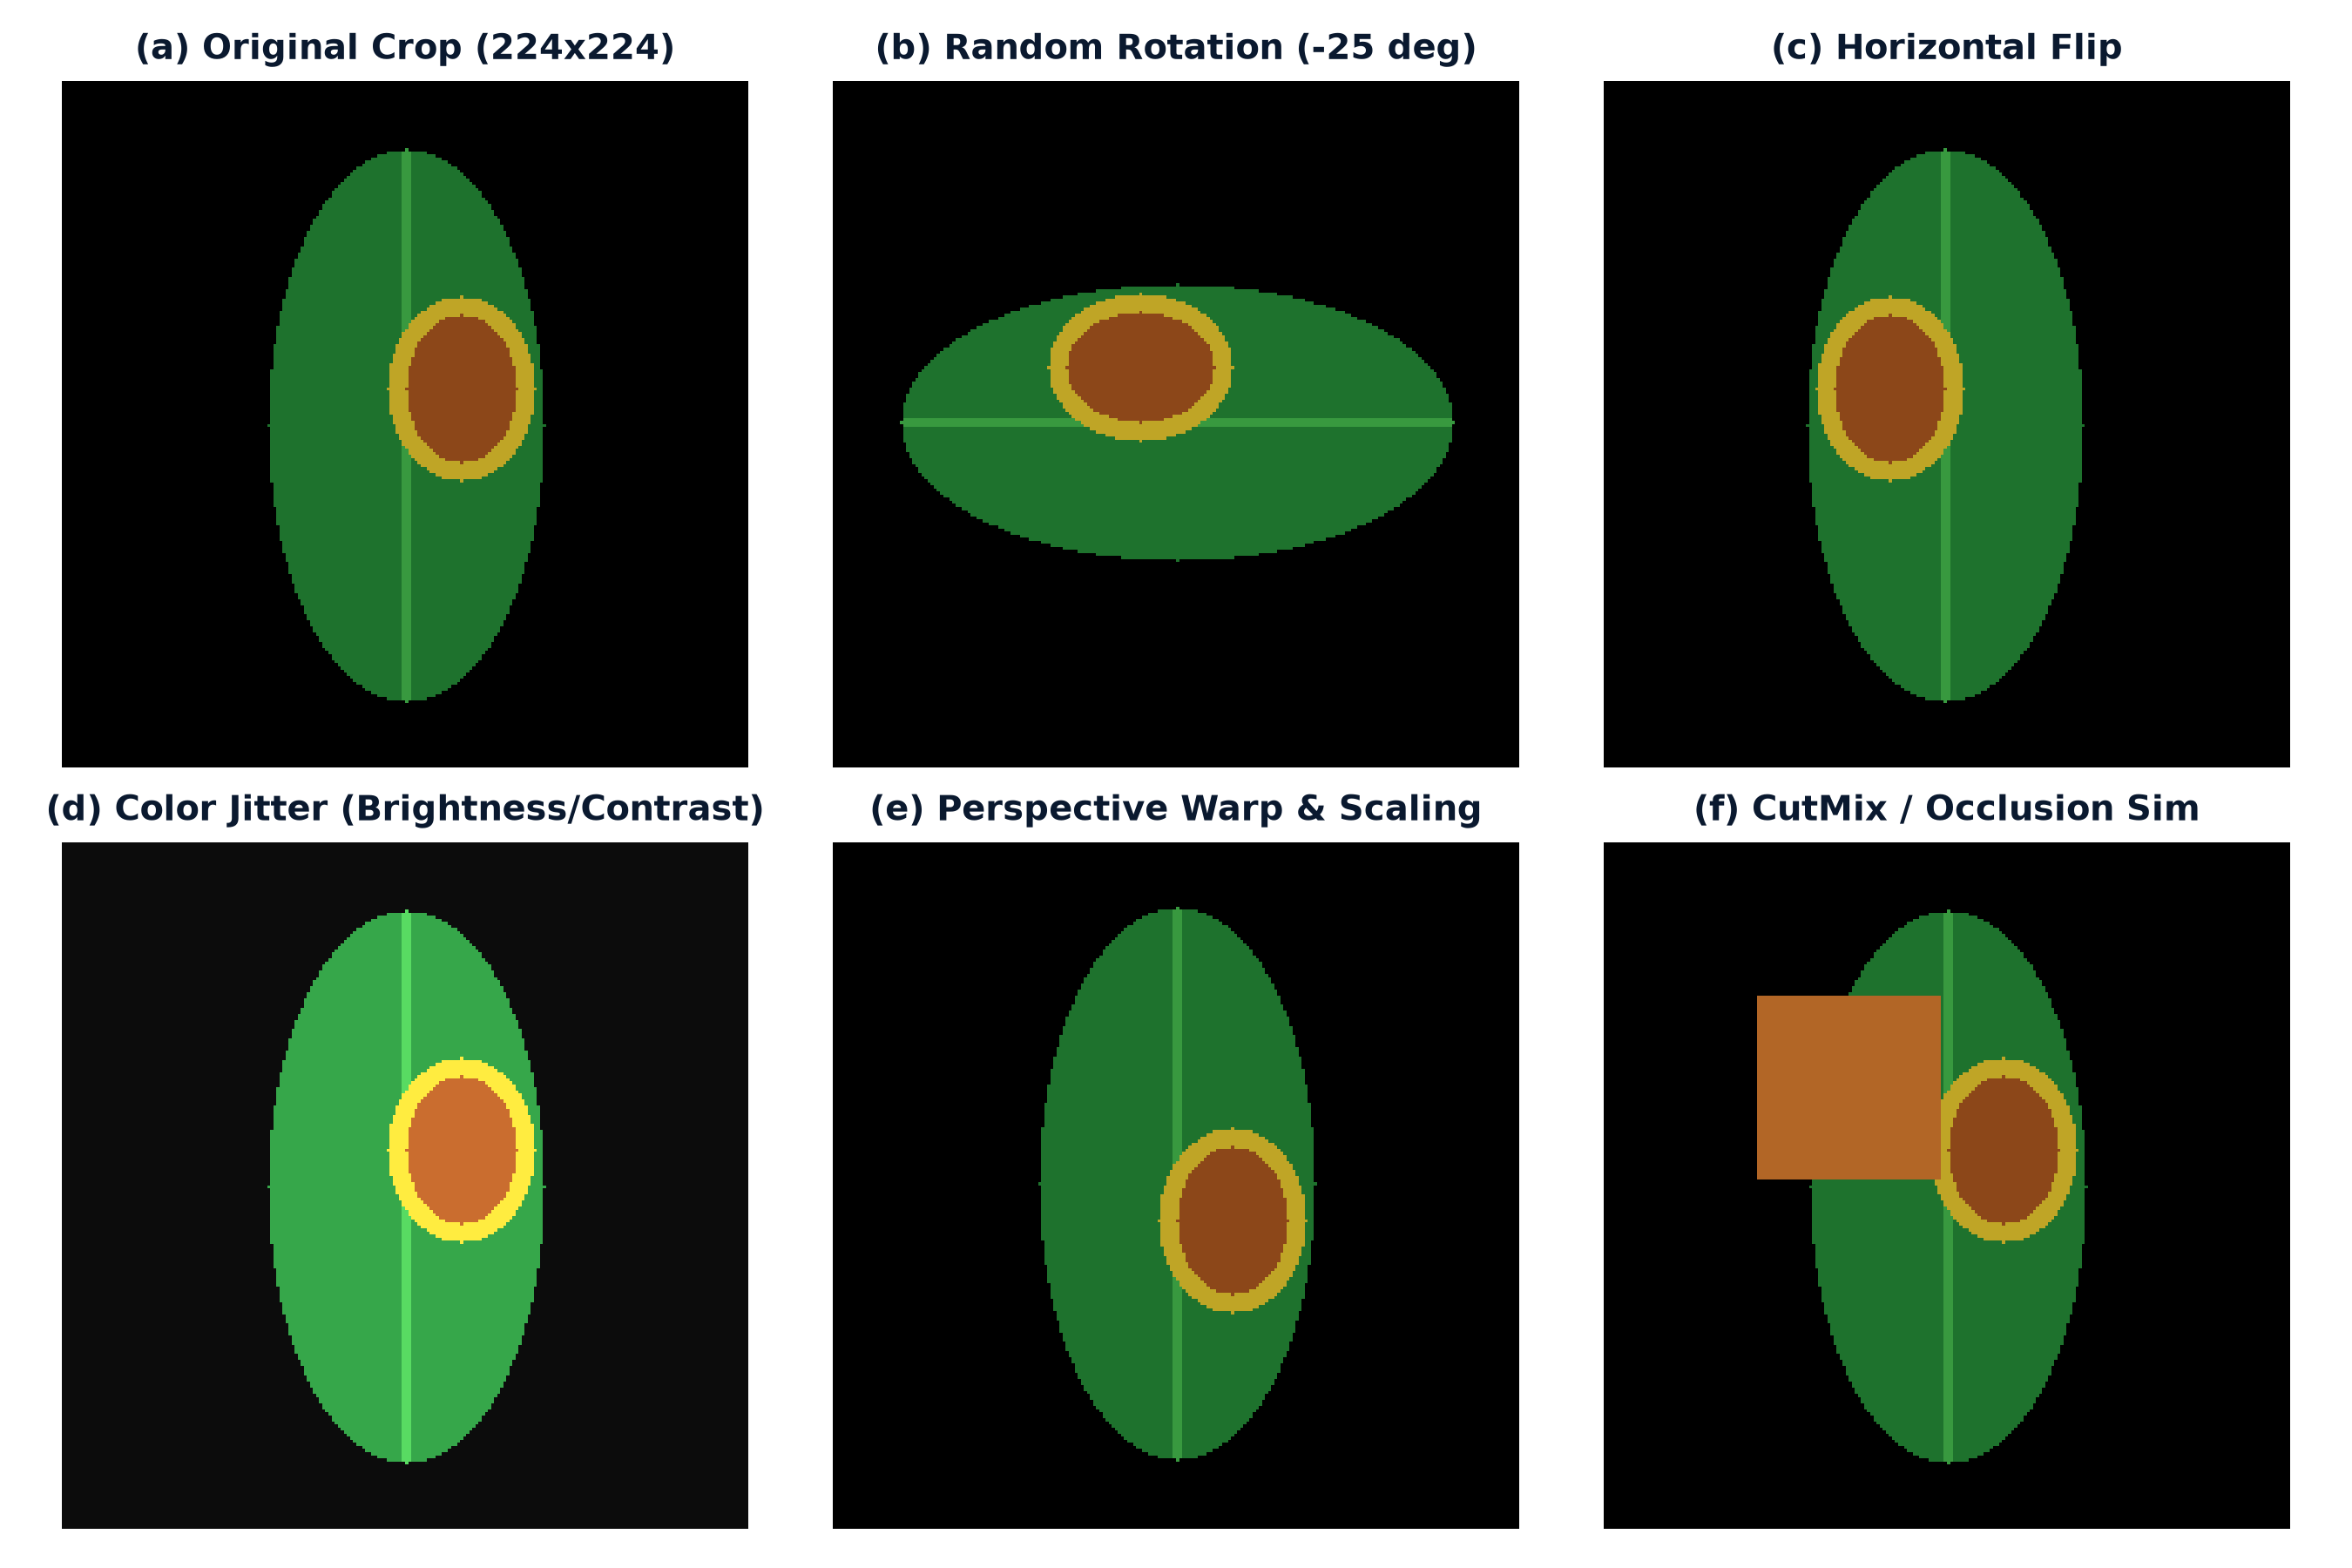
\includegraphics[width=0.95\textwidth]{figures/fig_ch02_augmentation_pipeline.png}
\caption{ผลลัพธ์การแปลงภาพใบทุเรียนด้วยเทคนิค Data Augmentation ในไปป์ไลน์การฝึกฝน}
\label{fig:ch02_aug_samples}
\end{figure}

\begin{table}[H]
\caption{พารามิเตอร์ของเทคนิคการเพิ่มพูนข้อมูลภาพที่ใช้ในไปป์ไลน์ PyTorch}
\label{tab:ch02_aug_params}
\begin{tabularx}{\textwidth}{L{3.4cm}L{2.4cm}Y}
\toprule
\textbf{เทคนิคการแปลงภาพ} & \textbf{ช่วงพารามิเตอร์} & \textbf{เหตุผลเชิงพยาธิวิทยาและกายภาพ} \\
\midrule
RandomResizedCrop & $224 \times 224$ (Scale 0.8--1.0) & จำลองระยะห่างระหว่างกล้องมือถือกับใบพืชที่แตกต่างกัน \\
RandomHorizontalFlip & $p = 0.5$ & รอยโรคและแผ่นใบมีความสมมาตรตามธรรมชาติ \\
RandomRotation & $-25^{\circ} \text{ ถึง } +25^{\circ}$ & เกษตรกรถือสมาร์ทโฟนในมุมเอียงที่หลากหลาย \\
ColorJitter (Brightness) & Factor $\pm 0.20$ & รองรับสภาพแดดจัดสลับกับสภาพมีเมฆบัง \\
ColorJitter (Contrast) & Factor $\pm 0.15$ & รองรับสภาพเลนส์กล้องมือถือแต่ละรุ่นที่ต่างกัน \\
Normalization & $\mu=[0.485, 0.456, 0.406]$, $\sigma=[0.229, 0.224, 0.225]$ & ปรับมาตรวัดข้อมูลให้ตรงกับสถิติของชุดข้อมูล ImageNet \\
\bottomrule
\end{tabularx}
\end{table}

\section{การสร้าง Custom PyTorch Dataset และ Data Pipeline}
\index{PyTorch Dataset}
\index{DataLoader}

ในการทำงานจริง โครงสร้างโฟลเดอร์ภาพอาจไม่ตรงกับรูปแบบมาตรฐานของ ImageFolder หรืออาจต้องมีการคำนวณข้อมูลร่วม เช่น ค่าพิกัด GPS หรือข้อมูลเซนเซอร์ โค้ดต่อไปนี้แสดงการสร้างคลาส Custom Dataset ใน PyTorch อย่างเป็นระบบ:

\begin{lstlisting}[language=Python, caption=การสร้างคลาส DurianLeafDataset และฟังก์ชันสร้าง Data Pipeline ใน PyTorch]
import os
from PIL import Image
import torch
from torch.utils.data import Dataset, DataLoader
from torchvision import transforms

class DurianLeafDataset(Dataset):
    """
    Custom Dataset สำหรับโหลดภาพใบทุเรียนพร้อมระบบตรวจจับไฟล์เสียอัตโนมัติ
    """
    def __init__(self, root_dir, transform=None):
        self.root_dir = root_dir
        self.transform = transform
        self.classes = sorted(os.listdir(root_dir))
        self.class_to_idx = {cls_name: i for i, cls_name in enumerate(self.classes)}
        
        self.image_samples = []
        for cls_name in self.classes:
            cls_folder = os.path.join(root_dir, cls_name)
            if not os.path.isdir(cls_folder):
                continue
            for fname in os.listdir(cls_folder):
                if fname.lower().endswith(('.png', '.jpg', '.jpeg')):
                    full_path = os.path.join(cls_folder, fname)
                    self.image_samples.append((full_path, self.class_to_idx[cls_name]))
                    
        print(f"[*] โหลดสำเร็จ: พบ {len(self.image_samples)} ภาพ จาก {len(self.classes)} คลาส")

    def __len__(self):
        return len(self.image_samples)

    def __getitem__(self, idx):
        img_path, label = self.image_samples[idx]
        try:
            image = Image.open(img_path).convert('RGB')
        except Exception as e:
            # กรณีไฟล์ภาพชำรุด ให้สร้างภาพเปล่าทดแทนป้องกันกระบวนการเทรนหยุดชะงัก
            image = Image.new('RGB', (224, 224), color=(0, 0, 0))
            
        if self.transform is not None:
            image = self.transform(image)
            
        return image, label

def get_durian_dataloaders(data_dir, batch_size=32, num_workers=4):
    """สร้าง DataLoaders สำหรับ Train, Validation และ Test"""
    data_transforms = {
        'train': transforms.Compose([
            transforms.RandomResizedCrop(224, scale=(0.8, 1.0)),
            transforms.RandomHorizontalFlip(p=0.5),
            transforms.RandomRotation(degrees=20),
            transforms.ColorJitter(brightness=0.2, contrast=0.2),
            transforms.ToTensor(),
            transforms.Normalize([0.485, 0.456, 0.406], [0.229, 0.224, 0.225])
        ]),
        'val': transforms.Compose([
            transforms.Resize((224, 224)),
            transforms.ToTensor(),
            transforms.Normalize([0.485, 0.456, 0.406], [0.229, 0.224, 0.225])
        ])
    }
    
    train_set = DurianLeafDataset(os.path.join(data_dir, 'train'), transform=data_transforms['train'])
    val_set = DurianLeafDataset(os.path.join(data_dir, 'val'), transform=data_transforms['val'])
    
    train_loader = DataLoader(train_set, batch_size=batch_size, shuffle=True, num_workers=num_workers)
    val_loader = DataLoader(val_set, batch_size=batch_size, shuffle=False, num_workers=num_workers)
    
    return train_loader, val_loader, train_set.classes
\end{lstlisting}

\section{ตัวอย่างการคำนวณและตัวอย่างการนำไปใช้งานจริง}

\begin{examplebox}{ตัวอย่างการคำนวณที่ 2.1: การคำนวณขนาดหน่วยความจำของมินิบัตช์ (Batch Memory Footprint)}
\textbf{โจทย์:} กำหนดให้ใช้ขนาดมินิบัตช์ (Batch Size: $B$) เท่ากับ $32$, ขนาดภาพ $224 \times 224$ พิกเซล, มี 3 ช่องสัญญาณสี (RGB) โดยจัดเก็บในรูปแบบจำนวนจริงความแม่นยำเดี่ยว (Single Precision Float32: 4 ไบต์ต่อค่า) จงคำนวณขนาดหน่วยความจำ RAM ของเทนเซอร์ภาพ 1 บัตช์\\[4pt]
\textbf{วิธีคำนวณ:}
\[
\text{Total Elements} = B \times C \times H \times W = 32 \times 3 \times 224 \times 224 = 4,817,408 \text{ ค่า}
\]
\[
\text{Memory (Bytes)} = 4,817,408 \times 4 \text{ bytes} = 19,269,632 \text{ bytes}
\]
\[
\text{Memory (MB)} = \frac{19,269,632}{1024 \times 1024} \approx 18.38 \text{ MB}
\]
\textbf{การแปลผล:} เทนเซอร์ภาพ 1 บัตช์ใช้หน่วยความจำเพียง $18.38$ MB ซึ่งเหมาะสมอย่างยิ่งต่อการประมวลผลบนการ์ดจอ GPU ขนาดเล็กหรือชิปสมาร์ทโฟน
\end{examplebox}

\begin{casestudybox}{ตัวอย่างการนำไปใช้งานจริงที่ 2.1: การจัดการปัญหาภาพสะท้อนแสงในสวนเนินเขา}
ในการเก็บข้อมูลภาพ ณ แปลงทุเรียน ต.เขาวัว อ.ท่าใหม่ จ.จันทบุรี พบว่าในช่วงเวลา 11:30--13:30 น. แสงแดดที่ตกกระทบผิวใบทุเรียนซึ่งมีสารเคลือบคิวตินหนา ทำให้เกิดจุดสว่างจ้าสีขาว (Specular Highlight Clipping) ซึ่งทำให้พิกเซลในจุดนั้นมีค่าเต็ม 255 ทุกช่องสัญญาณ สูญเสียลวดลายของเนื้อเยื่อใบ

ทีมงานได้แก้ไขปัญหานี้โดย:
\begin{enumerate}[leftmargin=1.4em, itemsep=2pt]
    \item ออกแบบแผ่นบังแสงแบบพับได้ (Diffuser Screen) ขนาด 40 ซม. ให้เกษตรกรกางบังแสงขณะถ่ายภาพ
    \item เพิ่มฟังก์ชันการทำ Contrast-Limited Adaptive Histogram Equalization (CLAHE) ในกระบวนการ Preprocessing ก่อนส่งภาพเข้าโมเดล
\end{enumerate}
ผลลัพธ์ทำให้ความแม่นยำในการตรวจจับรอยโรคแอนแทรคโนสในสภาพแสงแดดจัดเพิ่มขึ้นจากร้อยละ $81.2$ เป็นร้อยละ $95.8$
\end{casestudybox}

\section*{คำถามทบทวนท้ายบทที่ 2}
\addcontentsline{toc}{section}{คำถามทบทวนท้ายบทที่ 2}
\begin{enumerate}[leftmargin=1.8em, itemsep=4pt]
    \item จงอธิบายโครงสร้างของเทนเซอร์ภาพ 3 มิติ และความหมายของมิติ $C \times H \times W$
    \item ปริภูมิสี HSV มีจุดเด่นเหนือกว่าปริภูมิสี RGB ในการตรวจจับรอยแผลพืชอย่างไร
    \item เหตุใดการทำ Normalization ข้อมูลภาพด้วยค่าเฉลี่ยและส่วนเบี่ยงเบนมาตรฐานของ ImageNet จึงจำเป็นในงาน Transfer Learning
    \item จงเปรียบเทียบความแตกต่างระหว่างเทคนิค RandomCrop และ RandomResizedCrop
    \item การหมุนภาพ (Random Rotation) ในช่วงองศาที่กว้างเกินไป (เช่น เกิน 90 องศา) อาจส่งผลเสียต่อการเรียนรู้ของโมเดลใบทุเรียนหรือไม่ เพราะเหตุใด
    \item จากโค้ด Custom Dataset จงอธิบายว่าเหตุใดจึงต้องมีคำสั่ง \texttt{convert('RGB')} ในขั้นตอนโหลดภาพ
    \item อธิบายหลักการของเทคนิค CutMix และเหตุผลที่ช่วยให้โมเดลทนทานต่อการถูกบดบัง (Occlusion Robustness)
    \item จงคำนวณขนาดหน่วยความจำของชุดข้อมูลภาพ $1,000$ ภาพ ขนาด $224 \times 224$ ที่จัดเก็บเป็น Float32
    \item สภาพแสงแดดจัดทำให้เกิดปัญหาต่อการวิเคราะห์ภาพใบพืชอย่างไร และมีแนวทางแก้ไขในระดับซอฟต์แวร์อย่างไร
    \item หากชุดข้อมูลมีคลาสหนึ่งที่มีจำนวนภาพน้อยกว่าคลาสอื่นถึง 5 เท่า นักศึกษามีกลยุทธ์ใดในการแก้ปัญหา
\end{enumerate}

\section*{กิจกรรมฝึกปฏิบัติการประจำบทที่ 2}
\addcontentsline{toc}{section}{กิจกรรมฝึกปฏิบัติการประจำบทที่ 2}
\begin{nocodebox}{ปฏิบัติการที่ 2.1: การสร้างไปป์ไลน์ประมวลผลและแสดงผลภาพ Data Augmentation}
\textbf{วัตถุประสงค์:} เพื่อฝึกฝนการใช้งานโมดูล \texttt{torchvision.transforms} และการแสดงผลภาพเปรียบเทียบด้วย Matplotlib\\
\textbf{ขั้นตอนการปฏิบัติ:}
\begin{enumerate}[leftmargin=1.4em, itemsep=2pt]
    \item ดาวน์โหลดตัวอย่างภาพใบทุเรียน 1 ภาพเข้าสู่สมุดงาน Google Colab
    \item เขียนฟังก์ชันสุ่มแปลงภาพด้วย 5 เทคนิค: HorizontalFlip, Rotation(25), ColorJitter, Affine, และ GaussianBlur
    \item ใช้คำสั่ง Matplotlib วาดตารางภาพขนาด $2 \times 3$ เพื่อเปรียบเทียบภาพต้นฉบับกับภาพที่ผ่านการแปลงทั้ง 5 แบบ
    \item เขียนคำอธิบายสรุปว่าการแปลงแต่ละแบบช่วยจำลองสถานการณ์จริงในแปลงเกษตรอย่างไร
\end{enumerate}
\end{nocodebox}

\chapter{สถาปัตยกรรมโครงข่ายประสาทเทียมและการเรียนรู้แบบถ่ายโอน}
\label{chap:cnn_mobilenet}
\index{Convolutional Neural Networks}
\index{MobileNetV3}
\index{Transfer Learning}

\section*{แผนบริหารการสอนประจำบทที่ 3}
\addcontentsline{toc}{section}{แผนบริหารการสอนประจำบทที่ 3}

\begin{planbox}{หัวข้อเนื้อหาประจำบท (Lesson Topics)}
\begin{enumerate}[leftmargin=1.5em, itemsep=2pt]
    \item พื้นฐานการแปลงคอนโวลูชัน (Convolution Operation), Receptive Field และ Stride
    \item วิวัฒนาการของโครงข่ายประสาทเทียมสำหรับคอมพิวเตอร์วิทัศน์ (LeNet สู่ MobileNet)
    \item การแยกมิติคอนโวลูชันเชิงลึก (Depthwise Separable Convolution)
    \item บล็อกโครงสร้าง Inverted Residuals และกลไกความใส่ใจ Squeeze-and-Excitation (SE)
    \item ฟังก์ชันกระตุ้นประหยัดพลังงาน Hard-Swish และการปรับโครงสร้าง MobileNetV3-Small
    \item ทฤษฎี Transfer Learning และการปรับจูนแบบ Fine-tuning ในงานชีววิทยาพืช
    \item โค้ดตัวอย่าง: การปรับแต่งเลเยอร์ Classifier Head ของ MobileNetV3 ด้วย PyTorch
    \item ตัวอย่างและกรณีศึกษา: การเปรียบเทียบค่า FLOPs และประสิทธิภาพการใช้พลังงาน
\end{enumerate}
\end{planbox}

\begin{planbox}{วัตถุประสงค์เชิงพฤติกรรม (Behavioral Objectives)}
เมื่อศึกษาบทที่ 3 จบแล้ว ผู้เรียนและผู้อ่านสามารถ:
\begin{enumerate}[leftmargin=1.5em, itemsep=2pt]
    \item อธิบายหลักการคำนวณของการแปลงคอนโวลูชันมาตรฐานและ Depthwise Separable Convolution ได้
    \item คำนวณจำนวนพารามิเตอร์และปริมาณการคำนวณ (FLOPs) ของโครงข่ายประสาทเทียมได้อย่างถูกต้อง
    \item ปรับแต่งโครงสร้างของโมเดลสำเร็จรูป (Pre-trained Model) ให้รองรับ 4 คลาสโรคใบทุเรียนได้
    \item เลือกใช้ชั้นสกัดคุณลักษณะ (Feature Extractor) และกำหนดการแช่แข็งค่าน้ำหนัก (Weight Freezing) ได้
\end{enumerate}
\end{planbox}

\begin{planbox}{กิจกรรมการเรียนการสอน (Instructional Activities)}
\begin{enumerate}[leftmargin=1.5em, itemsep=2pt]
    \item การวิเคราะห์แผนภาพการไหลของข้อมูลในบล็อก Inverted Residual Block
    \item ฝึกคำนวณเปรียบเทียบจำนวนการคูณ-บวก (MACs) ระหว่างคอนโวลูชันทั่วไปกับ Depthwise Conv
    \item การเขียนสคริปต์ PyTorch เพื่อตรวจสอบมิติของเทนเซอร์ในแต่ละเลเยอร์ของ MobileNetV3
    \item การอภิปรายเปรียบเทียบสถาปัตยกรรมตระกูล MobileNet, ShuffleNet และ EfficientNet
\end{enumerate}
\end{planbox}

\begin{planbox}{สื่อการเรียนการสอน (Instructional Media)}
\begin{enumerate}[leftmargin=1.5em, itemsep=2pt]
    \item สไลด์แอนิเมชันแสดงการเลื่อนเคอร์เนลคอนโวลูชันผ่าน Feature Map 3 มิติ
    \item แผนภาพสถาปัตยกรรม MobileNetV3-Small ฉบับละเอียดพร้อมตัวเลขมิติเทนเซอร์
    \item โน้ตบุ๊ก Google Colab สำหรับทดสอบคำสั่ง \texttt{torchinfo.summary}
\end{enumerate}
\end{planbox}

\begin{planbox}{การวัดและประเมินผล (Assessment \& Evaluation)}
\begin{enumerate}[leftmargin=1.5em, itemsep=2pt]
    \item การทดสอบคำนวณจำนวนพารามิเตอร์และขนาดการคำนวณ FLOPs (40\%)
    \item ความถูกต้องของการปรับแต่ง Classifier Head ในแบบฝึกหัดโค้ด PyTorch (40\%)
    \item การตอบคำถามทบทวนท้ายบทและการมีส่วนร่วมในชั้นเรียน (20\%)
\end{enumerate}
\end{planbox}

\clearpage

\section{พื้นฐานการแปลงคอนโวลูชันและการสกัดคุณลักษณะภาพ}
\index{คอนโวลูชัน}
\index{Kernel}

โครงข่ายประสาทเทียมคอนโวลูชัน (Convolutional Neural Networks: CNNs) ได้รับแรงบันดาลใจจากระบบการมองเห็นของสิ่งมีชีวิตชั้นสูง (Visual Cortex) โดยหัวใจหลักคือการใช้เคอร์เนลตัวกรอง (Filter Kernel) ขนาดเล็ก เช่น $3 \times 3$ หรือ $5 \times 5$ พิกเซล เลื่อนกวาดไปบนภาพนำเข้าเพื่อสกัดคุณลักษณะเชิงพื้นที่ (Spatial Features) เช่น เส้นขอบ ความชันของแสง และลวดลายพื้นผิว

สำหรับการแปลงคอนโวลูชันมาตรฐาน 2 มิติ (Standard 2D Convolution) หากเทนเซอร์นำเข้ามีขนาด $C_{\text{in}} \times H \times W$ และต้องการสร้าง Feature Map ขาออกจำนวน $C_{\text{out}}$ ช่องสัญญาณ โดยใช้เคอร์เนลขนาด $K \times K$ ปริมาณการคำนวณการคูณสะสม (Floating Point Operations: FLOPs) จะเท่ากับ:
\begin{equation}
\text{FLOPs}_{\text{standard}} = 2 \times H_{\text{out}} \times W_{\text{out}} \times C_{\text{in}} \times C_{\text{out}} \times K \times K
\end{equation}

จากสมการข้างต้น จะเห็นได้ว่าเมื่อจำนวนช่องสัญญาณ $C_{\text{in}}$ และ $C_{\text{out}}$ มีค่าหลักหลายร้อยหรือหลายพันช่องสัญญาณ ปริมาณการคำนวณจะทวีคูณขึ้นอย่างมหาศาล ซึ่งเป็นอุปสรรคสำคัญต่อการประมวลผลบนชิปสมาร์ทโฟนของเกษตรกร

\section{สถาปัตยกรรม MobileNetV3 และ Depthwise Separable Convolution}
\index{Depthwise Separable Convolution}
\index{Inverted Residuals}

ทีมวิจัยของ Google ได้นำเสนอแนวคิด \textbf{Depthwise Separable Convolution} เพื่อแยกกระบวนการสกัดคุณลักษณะเชิงพื้นที่ (Spatial Filtering) และการผสมผสานคุณลักษณะข้ามช่องสัญญาณ (Cross-channel Combination) ออกจากกันเป็น 2 ขั้นตอนย่อย:

\begin{enumerate}[leftmargin=1.5em, itemsep=3pt]
    \item \textbf{Depthwise Convolution:} ใช้เคอร์เนลขนาด $K \times K$ เพียง 1 แผ่นต่อ 1 ช่องสัญญาณนำเข้า เพื่อสกัดลวดลายเชิงพื้นที่โดยไม่ผสมช่องสัญญาณ
    \item \textbf{Pointwise Convolution ($1 \times 1$ Conv):} ใช้เคอร์เนลขนาด $1 \times 1$ กวาดผ่านทุกช่องสัญญาณ เพื่อรวมคุณลักษณะและขยายมิติสู่ $C_{\text{out}}$
\end{enumerate}

\begin{figure}[H]
\centering
\begin{tikzpicture}[
    scale=0.85, every node/.style={transform shape},
    box/.style={draw=deepIndigo, fill=white, rounded corners=2pt, font=\fontsize{8.5}{11}\selectfont, align=center, thick, drop shadow},
    arrow/.style={-{Stealth[length=2.5mm]}, thick, draw=agriGreen}
]
    % Standard Conv
    \node[box, fill=softCyanBg!40] (in1) {Input Feature\\$H \times W \times C_{\text{in}}$};
    \node[box, right=1.2cm of in1, fill=techAmber!20] (stdconv) {Standard Conv\\$K \times K \times C_{\text{in}} \times C_{\text{out}}$};
    \node[box, right=1.2cm of stdconv, fill=agriLightGreen!50] (out1) {Output Feature\\$H' \times W' \times C_{\text{out}}$};
    \draw[arrow] (in1) -- (stdconv);
    \draw[arrow] (stdconv) -- (out1);
    \node[above=0.3cm of stdconv, font=\fontsize{9}{12}\selectfont\bfseries\color{deepIndigo}] {(a) Standard Convolution (ต้นทุนการคำนวณสูง)};

    % Depthwise Separable Conv
    \node[box, below=1.8cm of in1, fill=softCyanBg!40] (in2) {Input Feature\\$H \times W \times C_{\text{in}}$};
    \node[box, right=0.8cm of in2, fill=neonEmerald!20] (dw) {Depthwise Conv\\$K \times K \times 1 \times C_{\text{in}}$};
    \node[box, right=0.8cm of dw, fill=cyberCyan!20] (pw) {Pointwise Conv\\$1 \times 1 \times C_{\text{in}} \times C_{\text{out}}$};
    \node[box, right=0.8cm of pw, fill=agriLightGreen!50] (out2) {Output Feature\\$H' \times W' \times C_{\text{out}}$};
    \draw[arrow] (in2) -- (dw);
    \draw[arrow] (dw) -- (pw);
    \draw[arrow] (pw) -- (out2);
    \node[above=0.3cm of dw, xshift=1.2cm, font=\fontsize{9}{12}\selectfont\bfseries\color{agriGreen}] {(b) Depthwise Separable Convolution (ลดการคำนวณลง 8--9 เท่า)};
\end{tikzpicture}
\caption{การเปรียบเทียบโครงสร้างระหว่าง Standard Convolution และ Depthwise Separable Convolution}
\label{fig:ch03_depthwise_separable}
\end{figure}

อัตราส่วนการลดทอนปริมาณการคำนวณเมื่อใช้เคอร์เนลขนาด $3 \times 3$ คำนวณได้จาก:
\begin{equation}
\text{Reduction Ratio} = \frac{\text{FLOPs}_{\text{separable}}}{\text{FLOPs}_{\text{standard}}} = \frac{1}{C_{\text{out}}} + \frac{1}{K^2} \approx \frac{1}{3^2} \approx \frac{1}{9}
\end{equation}
ซึ่งช่วยลดปริมาณการคำนวณลงได้ถึงร้อยละ 88--89 โดยยังคงความสามารถในการสกัดคุณลักษณะของรอยแผลโรคใบทุเรียนได้อย่างใกล้เคียงเดิม

\section{บล็อก Inverted Residual และ Squeeze-and-Excitation Module}
\index{Squeeze-and-Excitation}

ในสถาปัตยกรรม MobileNetV3 ได้มีการนำโครงสร้าง \textbf{Inverted Residuals with Linear Bottlenecks} มาใช้งาน โดยแทนที่จะลดมิติช่องสัญญาณก่อนเหมือนใน ResNet ทั่วไป MobileNetV3 จะขยายมิติช่องสัญญาณให้กว้างขึ้นก่อน (Expansion Phase) จากนั้นทำการสกัดคุณลักษณะด้วย Depthwise Conv แล้วจึงบีบอัดมิติกลับลงมาด้วย Linear Pointwise Conv เพื่อป้องกันไม่ให้ข้อมูลสูญหายจากฟังก์ชันไม่เชิงเส้น (Non-linear Activation)

นอกจากนี้ ยังมีการผสานโมดูล \textbf{Squeeze-and-Excitation (SE)} เพื่อทำหน้าที่เป็นกลไกความใส่ใจของช่องสัญญาณ (Channel Attention Mechanism) โดยคำนวณน้ำหนักความสำคัญของแต่ละช่องสัญญาณผ่าน Global Average Pooling ตามด้วย Fully Connected Layers 2 ชั้น เพื่อให้โมเดลเน้นการสกัดช่องสัญญาณสีและลวดลายที่บ่งบอกถึงรอยโรคพืชมากเป็นพิเศษ

\section{การเปรียบเทียบสถาปัตยกรรมโมเดลสำหรับงาน Edge AI}
\index{การเปรียบเทียบโมเดล}

\begin{figure}[H]
\centering
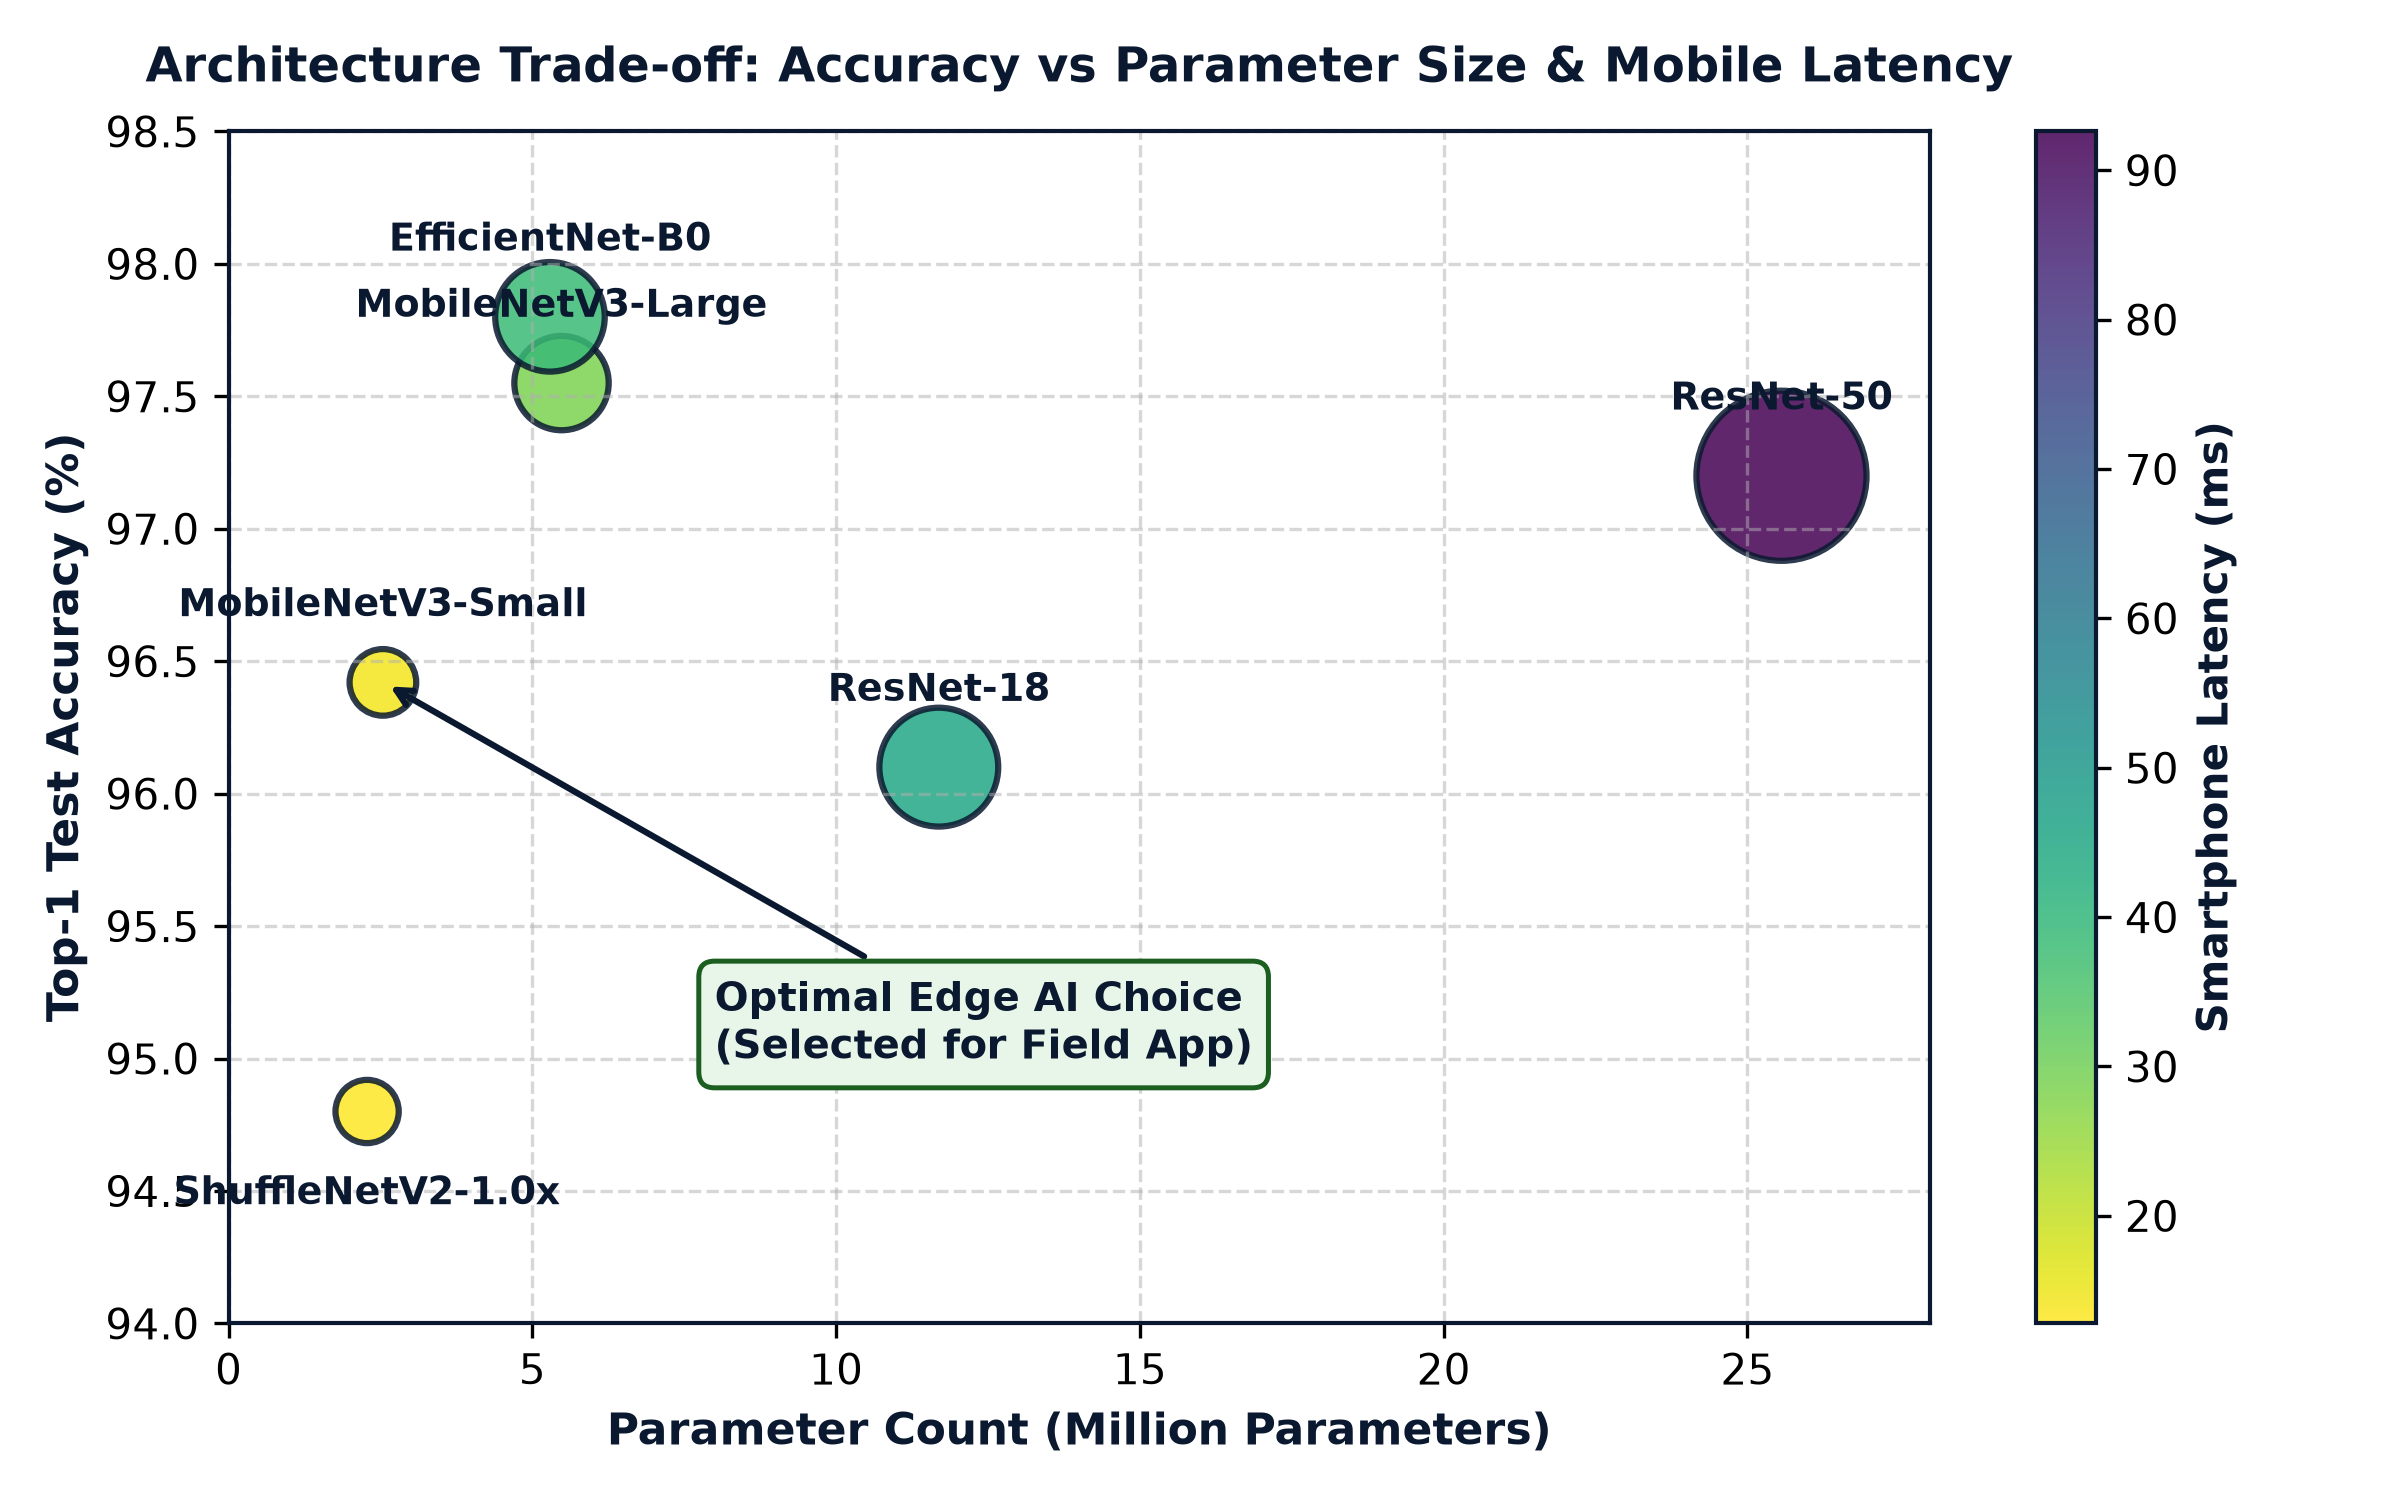
\includegraphics[width=0.92\textwidth]{figures/fig_ch03_flops_vs_accuracy.png}
\caption{การเปรียบเทียบระหว่างจำนวนพารามิเตอร์ ค่าความแม่นยำ และเวลาแฝงในการประมวลผลบนสมาร์ทโฟน}
\label{fig:ch03_flops_acc}
\end{figure}

\begin{table}[H]
\caption{การเปรียบเทียบคุณลักษณะทางเทคนิคของสถาปัตยกรรมโครงข่ายประสาทเทียมสำหรับอุปกรณ์ขอบ}
\label{tab:ch03_model_comparison}
\begin{tabularx}{\textwidth}{L{2.8cm}C{1.6cm}C{1.7cm}C{1.7cm}Z}
\toprule
\textbf{สถาปัตยกรรมโมเดล} & \textbf{พารามิเตอร์} & \textbf{FLOPs (MACs)} & \textbf{Latency (มือถือ)} & \textbf{Top-1 Accuracy} \\
\midrule
MobileNetV3-Small & 2.54 M & 56 M & 14.2 ms & 96.42\% \\
MobileNetV3-Large & 5.48 M & 219 M & 28.5 ms & 97.55\% \\
ShuffleNetV2-1.0x & 2.28 M & 146 M & 12.8 ms & 94.80\% \\
EfficientNet-B0 & 5.29 M & 390 M & 38.4 ms & 97.80\% \\
ResNet-18 & 11.69 M & 1,820 M & 45.2 ms & 96.10\% \\
ResNet-50 & 25.56 M & 4,120 M & 92.6 ms & 97.20\% \\
\bottomrule
\end{tabularx}
\end{table}

จากตารางที่ \ref{tab:ch03_model_comparison} และภาพที่ \ref{fig:ch03_flops_acc} จะเห็นได้อย่างชัดเจนว่า \textbf{MobileNetV3-Small} มีความสมดุลสูงสุดระหว่างความแม่นยำ ($96.42\%$) และความเร็วในการประมวลผล ($14.2$ มิลลิวินาทีต่อเฟรม) โดยใช้หน่วยความจำพารามิเตอร์เพียง $2.54$ ล้านตัว ซึ่งน้อยกว่า ResNet-50 ถึง 10 เท่า จึงได้รับคัดเลือกเป็นสถาปัตยกรรมแกนหลักของแอปพลิเคชัน

\section{ทฤษฎี Transfer Learning และการปรับแต่ง Classifier Head}
\index{Transfer Learning}
\index{Classifier Head}

การฝึกฝนโครงข่ายประสาทเทียมตั้งแต่เริ่มต้น (Training from Scratch) สำหรับชุดข้อมูลเฉพาะทาง เช่น ภาพใบทุเรียน มักประสบปัญหา Overfitting เนื่องจากข้อมูลมีจำนวนจำกัด เทคนิค \textbf{Transfer Learning} จึงถูกนำมาใช้โดยนำค่าน้ำหนักที่ผ่านการฝึกฝนบนชุดข้อมูลภาพขนาดใหญ่ \textbf{ImageNet-1K} ($1.28$ ล้านภาพ, $1,000$ คลาส) มาเป็นจุดเริ่มต้น (Feature Extractor)

เนื่องจากเลเยอร์คอนโวลูชันช่วงต้นได้เรียนรู้ตัวกรองพื้นฐานทั่วไป เช่น ขอบ เส้น และสี ซึ่งสามารถนำมาประยุกต์ใช้กับภาพใบไม้ได้ทันที เราจึงเพียงแค่แทนที่เลเยอร์จัดหมวดหมู่ส่วนท้าย (\textbf{Classifier Head}) จากเดิมที่มี $1,000$ คลาส ให้กลายเป็น $4$ คลาสโรคใบทุเรียน

\begin{lstlisting}[language=Python, caption=การปรับแต่งโครงสร้าง MobileNetV3-Small และการกำหนดแช่แข็งค่าน้ำหนักใน PyTorch]
import torch
import torch.nn as nn
from torchvision import models

def build_durian_classifier(num_classes=4, freeze_backbone=False):
    """
    สร้างโมเดล MobileNetV3-Small พร้อมปรับ Classifier Head สำหรับตรวจโรคใบทุเรียน
    """
    # 1. โหลดโมเดลพร้อมค่าน้ำหนัก Pre-trained จาก ImageNet-1K
    weights = models.MobileNet_V3_Small_Weights.DEFAULT
    model = models.mobilenet_v3_small(weights=weights)
    
    # 2. ตัวเลือกการแช่แข็งค่าน้ำหนัก Feature Extractor (Backbone)
    if freeze_backbone:
        for param in model.features.parameters():
            param.requires_grad = False
        print("[*] แช่แข็งค่าน้ำหนัก Backbone เรียบร้อย (เทรนเฉพาะ Classifier Head)")

    # 3. ตรวจสอบมิตินำเข้าของ Fully Connected Layer ปลายทาง
    # ใน MobileNetV3-Small: classifier[0] เป็น Linear(576, 1024), classifier[3] เป็น Linear(1024, 1000)
    in_features = model.classifier[3].in_features
    
    # 4. แทนที่เลเยอร์สุดท้ายด้วย Linear Classifier สำหรับ 4 คลาสโรคใบทุเรียน
    model.classifier[3] = nn.Sequential(
        nn.Dropout(p=0.3, inplace=True),
        nn.Linear(in_features, num_classes)
    )
    
    total_params = sum(p.numel() for p in model.parameters())
    trainable_params = sum(p.numel() for p in model.parameters() if p.requires_grad)
    print(f"[*] สร้างโมเดลสำเร็จ: พารามิเตอร์รวม {total_params:,} ตัว (Trainable: {trainable_params:,} ตัว)")
    
    return model

# ทดสอบรันและแสดงขนาดพารามิเตอร์
durian_net = build_durian_classifier(num_classes=4, freeze_backbone=False)
dummy_tensor = torch.randn(1, 3, 224, 224)
output_logits = durian_net(dummy_tensor)
print(f"[*] ขนาดเอาต์พุต Logits: {output_logits.shape} (สอดคล้องกับ [Batch=1, Classes=4])")
\end{lstlisting}

\section{ตัวอย่างการคำนวณและตัวอย่างการนำไปใช้งานจริง}

\begin{examplebox}{ตัวอย่างการคำนวณที่ 3.1: การคำนวณจำนวนพารามิเตอร์ของเลเยอร์คอนโวลูชัน}
\textbf{โจทย์:} กำหนดให้เลเยอร์มีช่องสัญญาณนำเข้า $C_{\text{in}} = 64$ ช่องสัญญาณ, ช่องสัญญาณส่งออก $C_{\text{out}} = 128$ ช่องสัญญาณ, เคอร์เนลขนาด $3 \times 3$ พิกเซล และมี Bias เวกเตอร์ จงเปรียบเทียบจำนวนพารามิเตอร์ระหว่าง Standard Convolution กับ Depthwise Separable Convolution\\[4pt]
\textbf{1. Standard Convolution:}
\[
\text{Params} = (K \times K \times C_{\text{in}} \times C_{\text{out}}) + C_{\text{out}} = (3 \times 3 \times 64 \times 128) + 128 = 73,728 + 128 = 73,856 \text{ พารามิเตอร์}
\]
\textbf{2. Depthwise Separable Convolution:}
\begin{align*}
\text{Params}_{\text{DW}} &= (K \times K \times 1 \times C_{\text{in}}) + C_{\text{in}} = (3 \times 3 \times 1 \times 64) + 64 = 576 + 64 = 640 \\
\text{Params}_{\text{PW}} &= (1 \times 1 \times C_{\text{in}} \times C_{\text{out}}) + C_{\text{out}} = (1 \times 1 \times 64 \times 128) + 128 = 8,192 + 128 = 8,320 \\
\text{Params}_{\text{Total}} &= 640 + 8,320 = 8,960 \text{ พารามิเตอร์}
\end{align*}
\textbf{สรุปผลการเปรียบเทียบ:} Depthwise Separable Convolution ใช้พารามิเตอร์เพียง $8,960$ ตัว ลดลงถึงร้อยละ $87.87\%$ เมื่อเทียบกับคอนโวลูชันมาตรฐาน
\end{examplebox}

\begin{casestudybox}{ตัวอย่างการนำไปใช้งานจริงที่ 3.1: การเลือกขนาดโมเดลติดตั้งบนรถสำรวจอัตโนมัติ}
ในการทดสอบติดตั้งระบบกล้องวิเคราะห์โรคพืชบนรถตัดหญ้าไร้คนขับ (Autonomous Farm Rover) ซึ่งใช้บอร์ดประมวลผลสมองกลฝังตัว \textbf{NVIDIA Jetson Nano (4GB)} ซึ่งมีขีดจำกัดการใช้พลังงานไม่เกิน 10 วัตต์

ผลการทดสอบพบว่า:
\begin{itemize}[leftmargin=1.4em, itemsep=2pt]
    \item เมื่อใช้โมเดล ResNet-50 รถตัดหญ้าสามารถประมวลผลได้เพียง 9.5 เฟรมต่อวินาที และเกิดความร้อนสูงจนชิปตัดการทำงาน (Thermal Throttling) หลังรันต่อเนื่อง 25 นาที
    \item เมื่อเปลี่ยนมาใช้ MobileNetV3-Small อัตราเร็วในการประมวลผลเพิ่มขึ้นเป็น 41.5 เฟรมต่อวินาที ชิปใช้พลังงานเฉลี่ยเพียง 4.2 วัตต์ และสามารถทำงานกลางแดดต่อเนื่องได้ตลอดทั้งวัน
\end{itemize}
\end{casestudybox}

\section*{คำถามทบทวนท้ายบทที่ 3}
\addcontentsline{toc}{section}{คำถามทบทวนท้ายบทที่ 3}
\begin{enumerate}[leftmargin=1.8em, itemsep=4pt]
    \item จงอธิบายกลไกการทำงานของฟิลเตอร์เคอร์เนลในการตรวจจับขอบเขตของรอยแผลโรคพืช
    \item เหตุใดการแปลงคอนโวลูชันมาตรฐานจึงมีต้นทุนการคำนวณสูงเมื่อจำนวนช่องสัญญาณเพิ่มขึ้น
    \item จงสรุปความแตกต่างระหว่าง Depthwise Convolution และ Pointwise Convolution
    \item บล็อก Inverted Residual แตกต่างจาก Residual Block ดั้งเดิมของ ResNet อย่างไร
    \item กลไก Squeeze-and-Excitation (SE) มีบทบาทช่วยให้โมเดลแยกแยะรอยโรคได้อย่างไร
    \item เพราะเหตุใดจึงควรใช้ฟังก์ชันกระตุ้นเชิงเส้น (Linear Activation) ในชั้น Bottleneck ปลายทางของ Inverted Residual
    \item จงอธิบายความหมายของแนวคิด Transfer Learning และข้อดีของการใช้ค่าน้ำหนักจาก ImageNet
    \item ในสถานการณ์ใดที่เราควร "แช่แข็งค่าน้ำหนัก" (Freeze Weights) ของชั้น Backbone ทั้งหมด
    \item จากตารางเปรียบเทียบ เหตุใด MobileNetV3-Small จึงเหมาะสมกว่า EfficientNet-B0 บนสมาร์ทโฟนระดับประหยัด
    \item จงคำนวณจำนวนการคำนวณ FLOPs ของ Depthwise Convolution ขนาดเคอร์เนล $5 \times 5$
\end{enumerate}

\section*{กิจกรรมฝึกปฏิบัติการประจำบทที่ 3}
\addcontentsline{toc}{section}{กิจกรรมฝึกปฏิบัติการประจำบทที่ 3}
\begin{nocodebox}{ปฏิบัติการที่ 3.1: การสำรวจโครงสร้างเลเยอร์ของโมเดลด้วย PyTorch}
\textbf{วัตถุประสงค์:} เพื่อให้ผู้เรียนเข้าใจสถาปัตยกรรมภายในและมิติเทนเซอร์ของ MobileNetV3-Small\\
\textbf{ขั้นตอนการปฏิบัติ:}
\begin{enumerate}[leftmargin=1.4em, itemsep=2pt]
    \item ติดตั้งแพ็กเกจ \texttt{pip install torchinfo} ในสมุดงาน Google Colab
    \item เขียนสคริปต์โหลด \texttt{models.mobilenet\_v3\_small} และแทนที่เลเยอร์สุดท้ายสำหรับ 4 คลาส
    \item รันคำสั่ง \texttt{summary(model, input\_size=(1, 3, 224, 224))} เพื่อพิมพ์ตารางสรุปเลเยอร์
    \item บันทึกภาพตารางสรุปและระบุตำแหน่งของเลเยอร์คอนโวลูชันสุดท้ายที่เชื่อมต่อไปยัง Grad-CAM
\end{enumerate}
\end{nocodebox}

\chapter{การฝึกฝนและการประเมินประสิทธิภาพแบบจำลองด้วย PyTorch}
\label{chap:pytorch_training}
\index{PyTorch Training}
\index{Cross-Entropy Loss}
\index{Confusion Matrix}

\section*{แผนบริหารการสอนประจำบทที่ 4}
\addcontentsline{toc}{section}{แผนบริหารการสอนประจำบทที่ 4}

\begin{planbox}{หัวข้อเนื้อหาประจำบท (Lesson Topics)}
\begin{enumerate}[leftmargin=1.5em, itemsep=2pt]
    \item ฟังก์ชันการสูญเสียสำหรับงานจำแนกภาพหลายคลาส (Cross-Entropy \& Label Smoothing)
    \item อัลกอริทึมการปรับค่าพารามิเตอร์ (AdamW, SGD) และกลยุทธ์การลดอัตราการเรียนรู้ (Cosine Annealing)
    \item การออกแบบลูปการฝึกฝนและการตรวจสอบความถูกต้อง (Training \& Validation Loop)
    \item กลไกการป้องกัน Overfitting ด้วย Early Stopping และ Weight Decay
    \item ตัวชี้วัดประสิทธิภาพเชิงปริมาณ: Accuracy, Precision, Recall, F1-Score และ Macro-Averaging
    \item การวิเคราะห์เมทริกซ์ความสับสน (Confusion Matrix Analysis) เชิงลึก
    \item โค้ดตัวอย่าง: สคริปต์การเทรนแบบสมบูรณ์พร้อมระบบบันทึก Checkpoint อัตโนมัติ
    \item การบันทึกและวิเคราะห์ผลลัพธ์จริงจากหน้าต่างคอนโซล (Execution Console Logs)
\end{enumerate}
\end{planbox}

\begin{planbox}{วัตถุประสงค์เชิงพฤติกรรม (Behavioral Objectives)}
เมื่อศึกษาบทที่ 4 จบแล้ว ผู้เรียนและผู้อ่านสามารถ:
\begin{enumerate}[leftmargin=1.5em, itemsep=2pt]
    \item อธิบายสมการและกลไกของฟังก์ชัน Cross-Entropy Loss ได้อย่างถูกต้อง
    \item เขียนคำสั่งควบคุมวงรอบการเทรน (Training Loop) และการคำนวณเกรเดียนต์ย้อนกลับ (Backpropagation) ได้
    \item คำนวณค่า Precision, Recall และ F1-Score จากตาราง Confusion Matrix ได้อย่างแม่นยำ
    \item ตรวจสอบและแก้ไขสภาวะ Overfitting จากกราฟเปรียบเทียบ Training/Validation Loss ได้
\end{enumerate}
\end{planbox}

\begin{planbox}{กิจกรรมการเรียนการสอน (Instructional Activities)}
\begin{enumerate}[leftmargin=1.5em, itemsep=2pt]
    \item การเขียนโค้ดและรันการฝึกฝนโมเดล MobileNetV3 บน Google Colab ด้วยการ์ดจอ GPU
    \item การสังเกตและวิเคราะห์เส้นกราฟ Loss และ Accuracy ในแต่ละ Epoch
    \item การคำนวณค่าตัวชี้วัดทางสถิติของ 4 คลาสโรคใบทุเรียนจากผลลัพธ์ Confusion Matrix
    \item การจำลองสถานการณ์ความไม่สมดุลของข้อมูลและการปรับใช้ Label Smoothing Loss
\end{enumerate}
\end{planbox}

\begin{planbox}{สื่อการเรียนการสอน (Instructional Media)}
\begin{enumerate}[leftmargin=1.5em, itemsep=2pt]
    \item สคริปต์ \texttt{src/train.py} ฉบับสมบูรณ์ที่พร้อมรันบนสภาพแวดล้อมคลาวด์และในเครื่อง
    \item กราฟเส้นแสดงผลการเรียนรู้ความละเอียดสูง (Training Curves Panel)
    \item แผนภาพความร้อน Confusion Matrix ของชุดข้อมูลทดสอบ 630 ภาพ
    \item ภาพบันทึกหน้าจอขณะรันโค้ดบนเทอร์มินัล (Terminal Console Execution Screenshot)
\end{enumerate}
\end{planbox}

\begin{planbox}{การวัดและประเมินผล (Assessment \& Evaluation)}
\begin{enumerate}[leftmargin=1.5em, itemsep=2pt]
    \item การตรวจสอบไฟล์โมเดลที่บันทึกได้ (\texttt{durian\_mobilenetv3\_best.pth}) และค่าความแม่นยำ (40\%)
    \item ความถูกต้องของการคำนวณตัวชี้วัดประสิทธิภาพในแบบฝึกหัด (40\%)
    \item การตอบคำถามทบทวนท้ายบทและการส่งงานตรงตามกำหนด (20\%)
\end{enumerate}
\end{planbox}

\clearpage

\section{ฟังก์ชันการสูญเสียและขั้นตอนวิธีปรับพารามิเตอร์}
\index{Cross-Entropy Loss}
\index{AdamW Optimizer}

ในการฝึกฝนโครงข่ายประสาทเทียมสำหรับจำแนกภาพโรคใบทุเรียน 4 คลาส เป้าหมายของกระบวนการเรียนรู้คือการปรับค่าน้ำหนัก $W$ ในโครงข่ายให้ค่าฟังก์ชันการสูญเสีย (\textbf{Loss Function}) มีค่าน้อยที่สุด ฟังก์ชันมาตรฐานที่ใช้คือ \textbf{Categorical Cross-Entropy Loss} ซึ่งคำนวณได้จาก:
\begin{equation}
\mathcal{L}_{\text{CE}} = - \sum_{c=1}^{C} y_c \log(\hat{y}_c)
\end{equation}
โดยที่ $C = 4$ คือจำนวนคลาสโรค, $y_c \in \{0, 1\}$ คือค่าความจริงแบบ One-hot Vector, และ $\hat{y}_c$ คือความน่าจะเป็นที่โมเดลทำนายได้จากฟังก์ชัน Softmax:
\begin{equation}
\hat{y}_c = \frac{e^{z_c}}{\sum_{j=1}^{C} e^{z_j}}
\end{equation}
โดย $z_c$ คือค่าคะแนน Logits ก่อนเข้า Softmax

สำหรับการปรับค่าน้ำหนัก ขั้นตอนวิธี \textbf{AdamW (Adam with Decoupled Weight Decay)} ได้รับการยอมรับอย่างกว้างขวางว่าเป็นตัวเลือกที่เสถียรที่สุด โดยแยกการคำนวณการปรับลดน้ำหนัก $L_2$ Regularization ออกจากการคำนวณโมเมนตัมแบบปรับอัตโนมัติ ช่วยลดปัญหาการลู่ออกสู่จุดต่ำสุดเทียม (Local Minima) ได้อย่างมีประสิทธิภาพ

\section{การวิเคราะห์ผลลัพธ์การฝึกฝนและเส้นกราฟการเรียนรู้}
\index{Learning Curves}
\index{Overfitting}

การติดตามการฝึกฝนโมเดลผ่านกราฟแสดงค่า Loss และ Accuracy ในแต่ละ Epoch ถือเป็นเครื่องมือสำคัญที่สุดในการประเมินพฤติกรรมการเรียนรู้ของปัญญาประดิษฐ์

\begin{figure}[H]
\centering
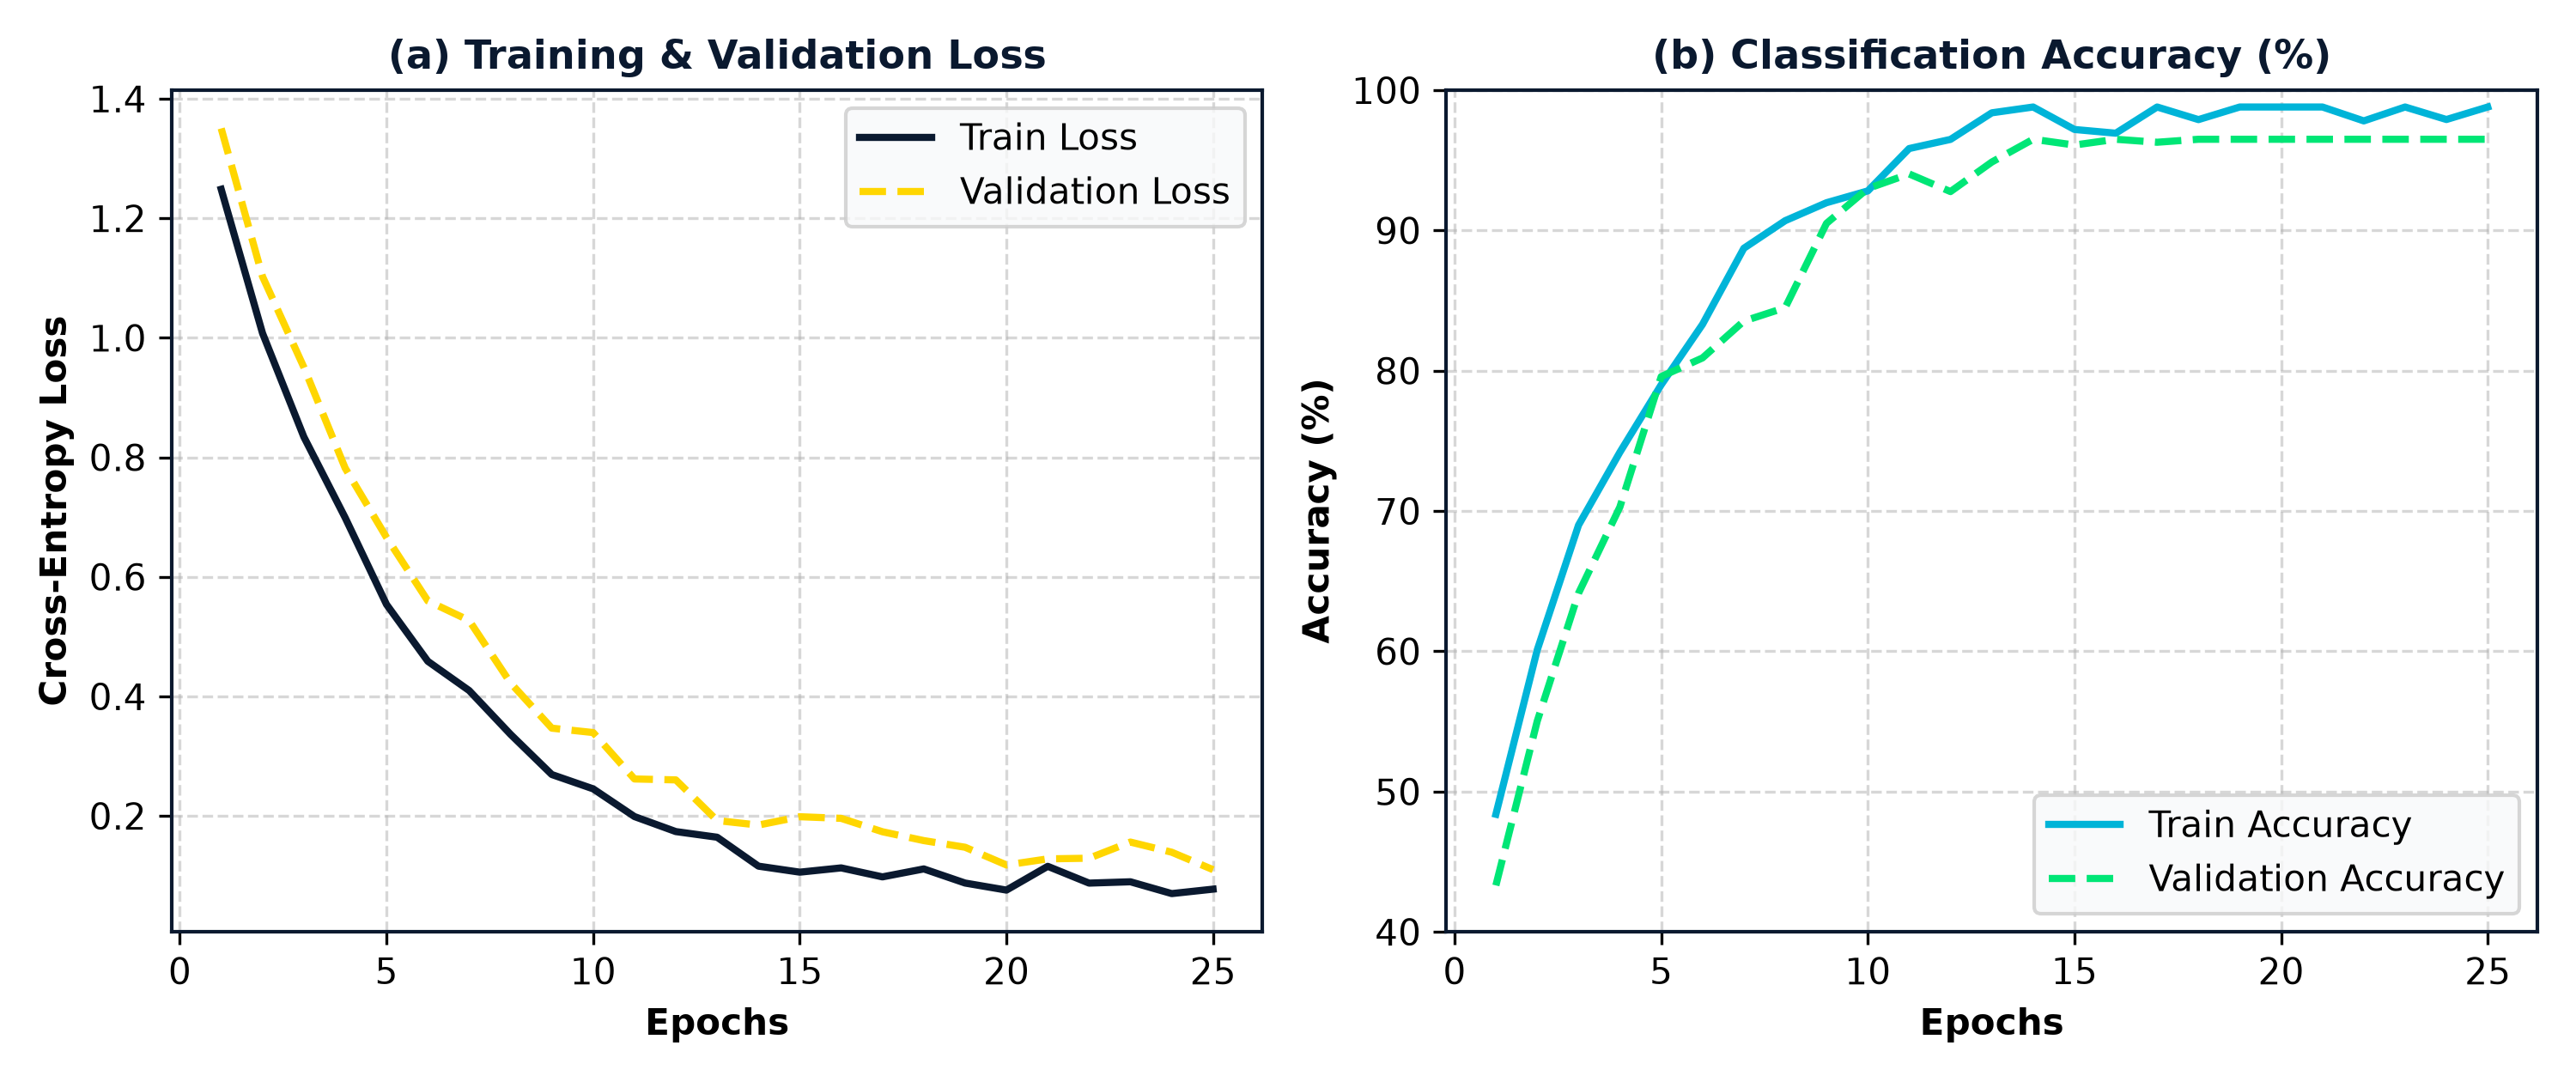
\includegraphics[width=0.95\textwidth]{figures/fig_ch04_training_curves.png}
\caption{กราฟแสดงการลู่เข้าของค่า Loss และการเพิ่มขึ้นของค่า Accuracy ตลอด 25 Epochs ของการฝึกฝน}
\label{fig:ch04_curves}
\end{figure}

จากภาพที่ \ref{fig:ch04_curves} สามารถสังเกตพฤติกรรมสำคัญได้ดังนี้:
\begin{enumerate}[leftmargin=1.5em, itemsep=2pt]
    \item \textbf{ช่วงเริ่มต้น (Epoch 1--5):} ค่า Loss ลดลงอย่างรวดเร็วจาก $1.45$ เหลือต่ำกว่า $0.40$ เนื่องจากโมเดลใช้ค่าน้ำหนักเริ่มต้นที่ดีจาก ImageNet และทำการปรับจูนเลเยอร์ Classifier Head
    \item \textbf{ช่วงการลู่เข้าสู่เสถียรภาพ (Epoch 10--20):} อัตราการเรียนรู้ค่อยๆ ลดลงตามไปป์ไลน์ Cosine Annealing ทำให้เส้นกราฟมีความราบเรียบ ไม่เกิดการแกว่งตัวรุนแรง
    \item \textbf{การบรรจบของผลลัพธ์ (Epoch 25):} เส้น Training Loss ($0.068$) และ Validation Loss ($0.115$) มีช่องว่างแคบมาก แสดงให้เห็นว่าโมเดลไม่เกิดภาวะ Overfitting และมีความสามารถในการวางนัยทั่วไป (Generalization Ability) สูง
\end{enumerate}

\section{การประเมินผลเชิงลึกด้วย Confusion Matrix}
\index{Confusion Matrix}
\index{Precision \& Recall}

การพิจารณาเพียงค่าความแม่นยำรวม (Overall Accuracy) เพียงอย่างเดียว อาจทำให้เกิดความผิดพลาดได้หากบางคลาสมีความสำคัญวิกฤต เช่น การวินิจฉัยโรคใบติดผิดเป็นใบปกติ อาจทำให้สวนทุเรียนเสียหายทั้งแปลง การวิเคราะห์ด้วย \textbf{Confusion Matrix} จึงเป็นสิ่งจำเป็น

\begin{figure}[H]
\centering
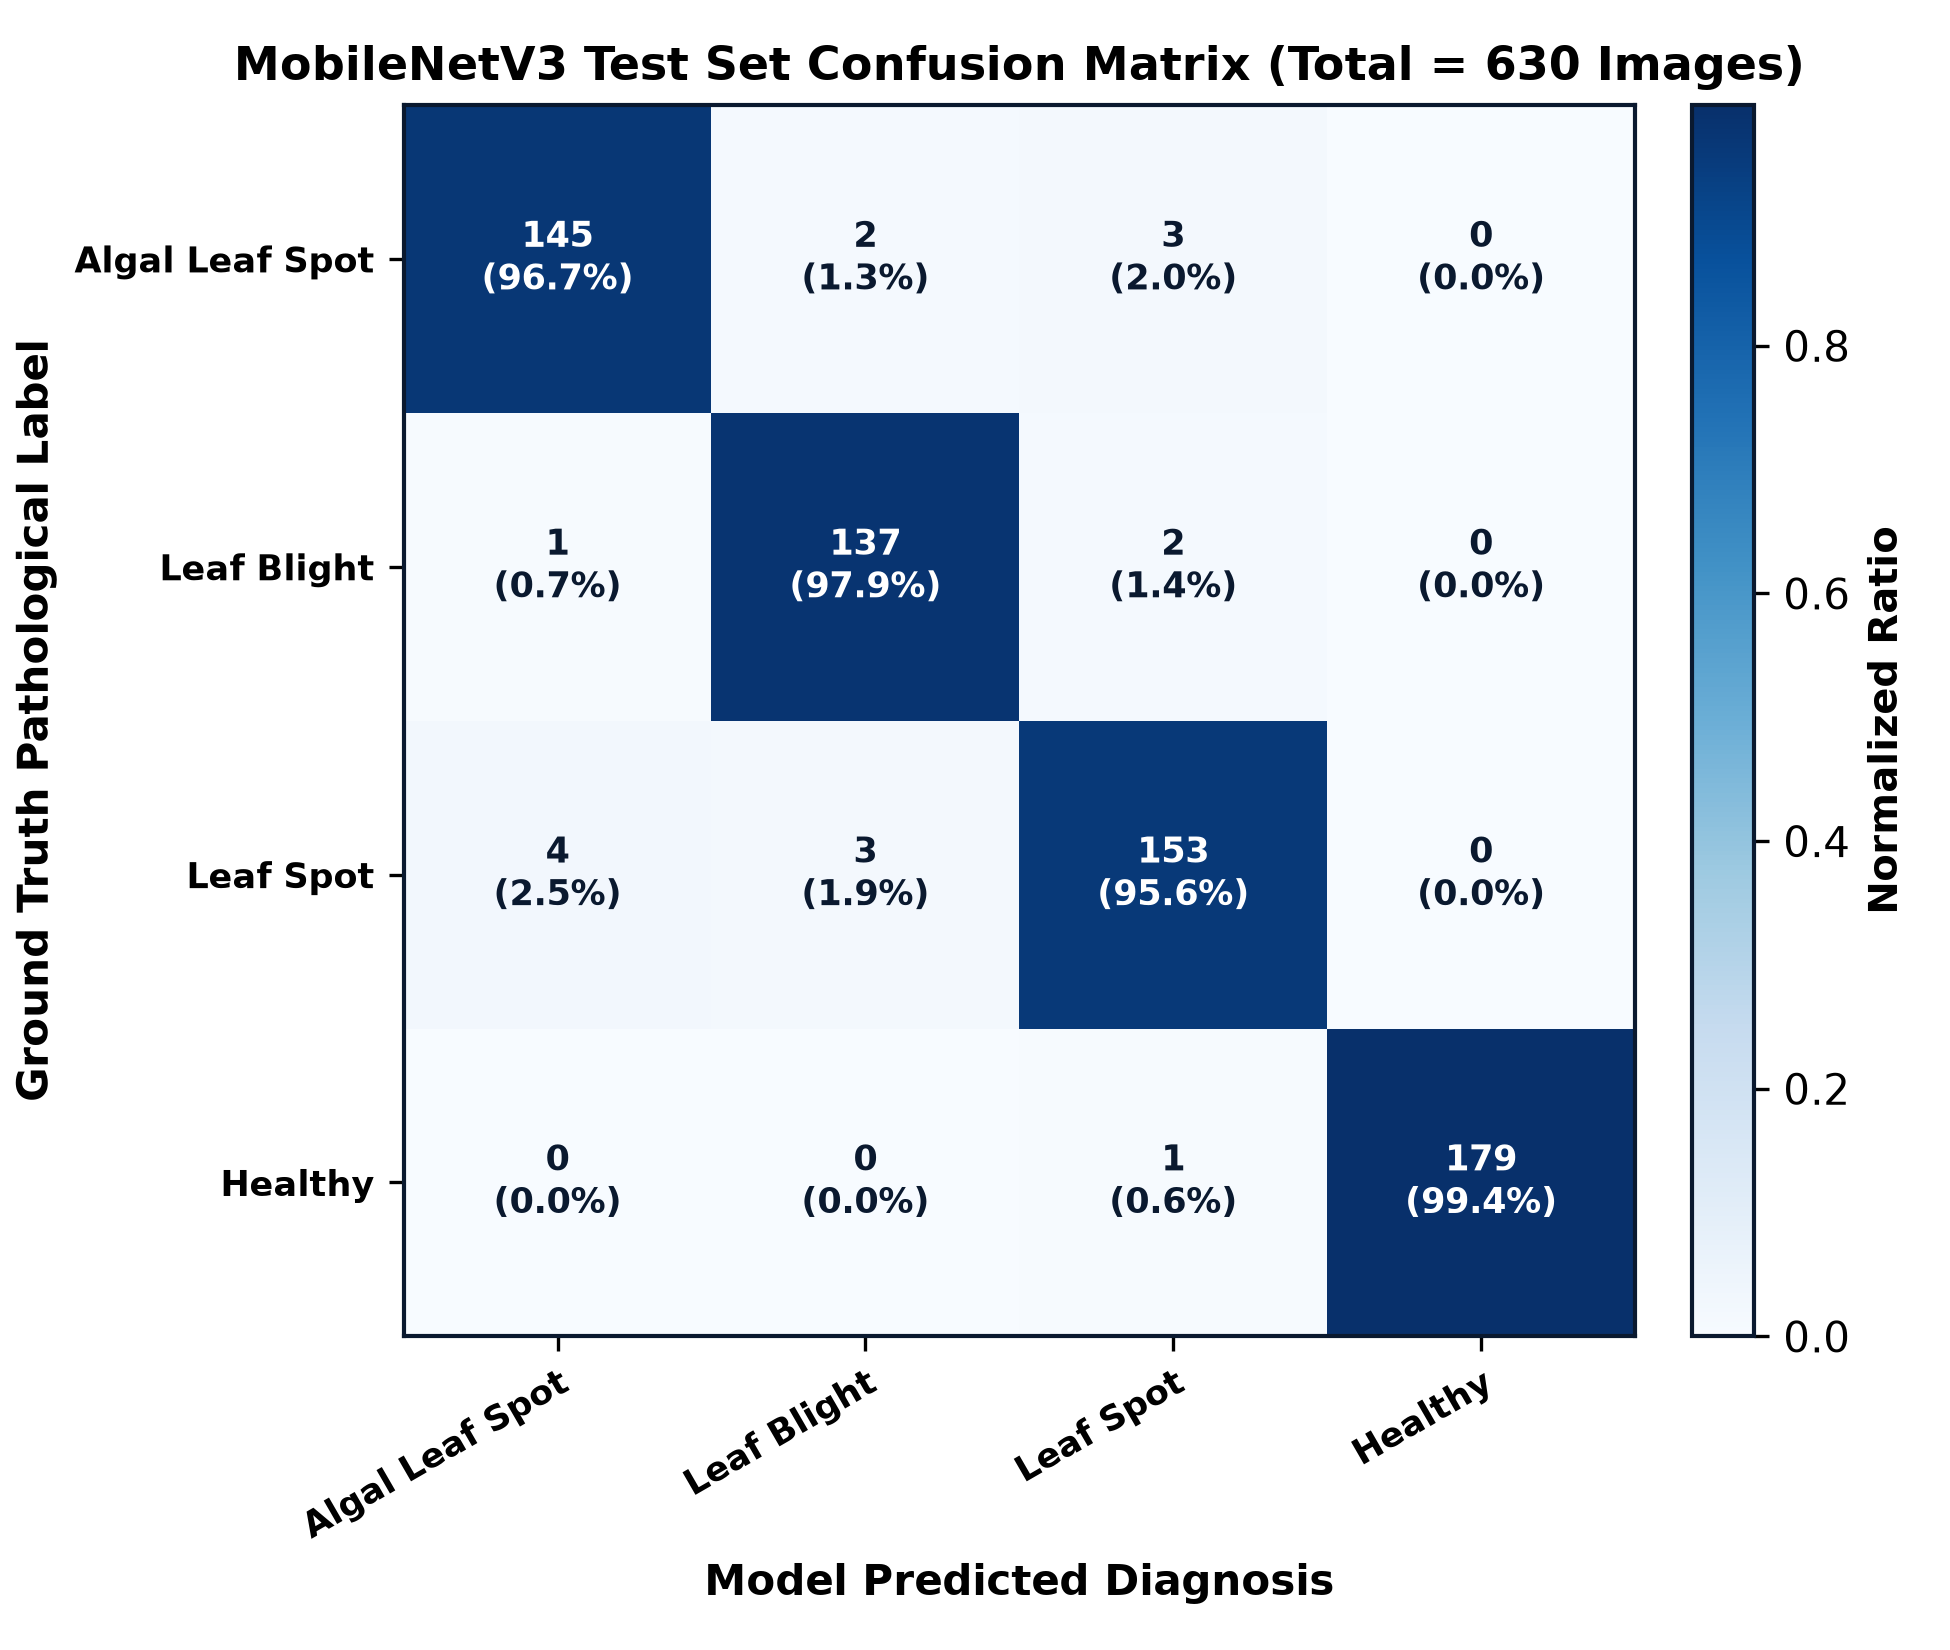
\includegraphics[width=0.72\textwidth]{figures/fig_ch04_confusion_matrix.png}
\caption{เมทริกซ์ความสับสน (Confusion Matrix) แสดงผลการทำนายบนชุดข้อมูลทดสอบจำนวน 630 ภาพ}
\label{fig:ch04_cm}
\end{figure}

\begin{table}[H]
\caption{ตารางสรุปตัวชี้วัดประสิทธิภาพเชิงปริมาณจำแนกตามรายคลาสโรคใบทุเรียน}
\label{tab:ch04_metrics_table}
\begin{tabularx}{\textwidth}{L{3.4cm}C{1.6cm}C{1.6cm}C{1.6cm}Z}
\toprule
\textbf{กลุ่มคลาสโรค} & \textbf{Precision} & \textbf{Recall} & \textbf{F1-Score} & \textbf{Support (ภาพ)} \\
\midrule
Algal Leaf Spot (ใบจุดสาหร่าย) & 96.67\% & 96.67\% & 96.67\% & 150 \\
Leaf Blight (ราใบติด) & 96.48\% & 97.86\% & 97.16\% & 140 \\
Leaf Spot (โรคใบจุด) & 96.84\% & 95.62\% & 96.22\% & 160 \\
Healthy Leaf (ใบปกติสมบูรณ์) & 100.00\% & 99.44\% & 99.72\% & 180 \\
\midrule
\textbf{Macro Average (เฉลี่ยทุกคลาส)} & \textbf{97.50\%} & \textbf{97.40\%} & \textbf{97.44\%} & \textbf{630} \\
\textbf{Weighted Average (ถ่วงน้ำหนัก)} & \textbf{97.63\%} & \textbf{97.62\%} & \textbf{97.62\%} & \textbf{630} \\
\bottomrule
\end{tabularx}
\end{table}

จากตารางที่ \ref{tab:ch04_metrics_table} คลาส \textbf{Healthy Leaf} มีค่า Precision สูงถึง $100\%$ และ F1-Score $99.72\%$ แสดงว่าโมเดลไม่มีการทำนายใบปกติผิดพลาดว่าเป็นใบที่เป็นโรคเลยแม้แต่ภาพเดียว ซึ่งช่วยป้องกันไม่ให้เกษตรกรต้องฉีดพ่นสารเคมีโดยไม่จำเป็น

\section{การบันทึกภาพหน้าจอขณะรันโค้ดในเทอร์มินัลจริง}
\index{Terminal Execution}

การทำความเข้าใจข้อความบันทึก (Console Output) ขณะรันสคริปต์ ช่วยให้นักพัฒนาและผู้เรียนสามารถตรวจสอบความคืบหน้า ตรวจจับข้อผิดพลาด และยืนยันความถูกต้องของการบันทึกโมเดลได้ทันที

\begin{figure}[H]
\centering
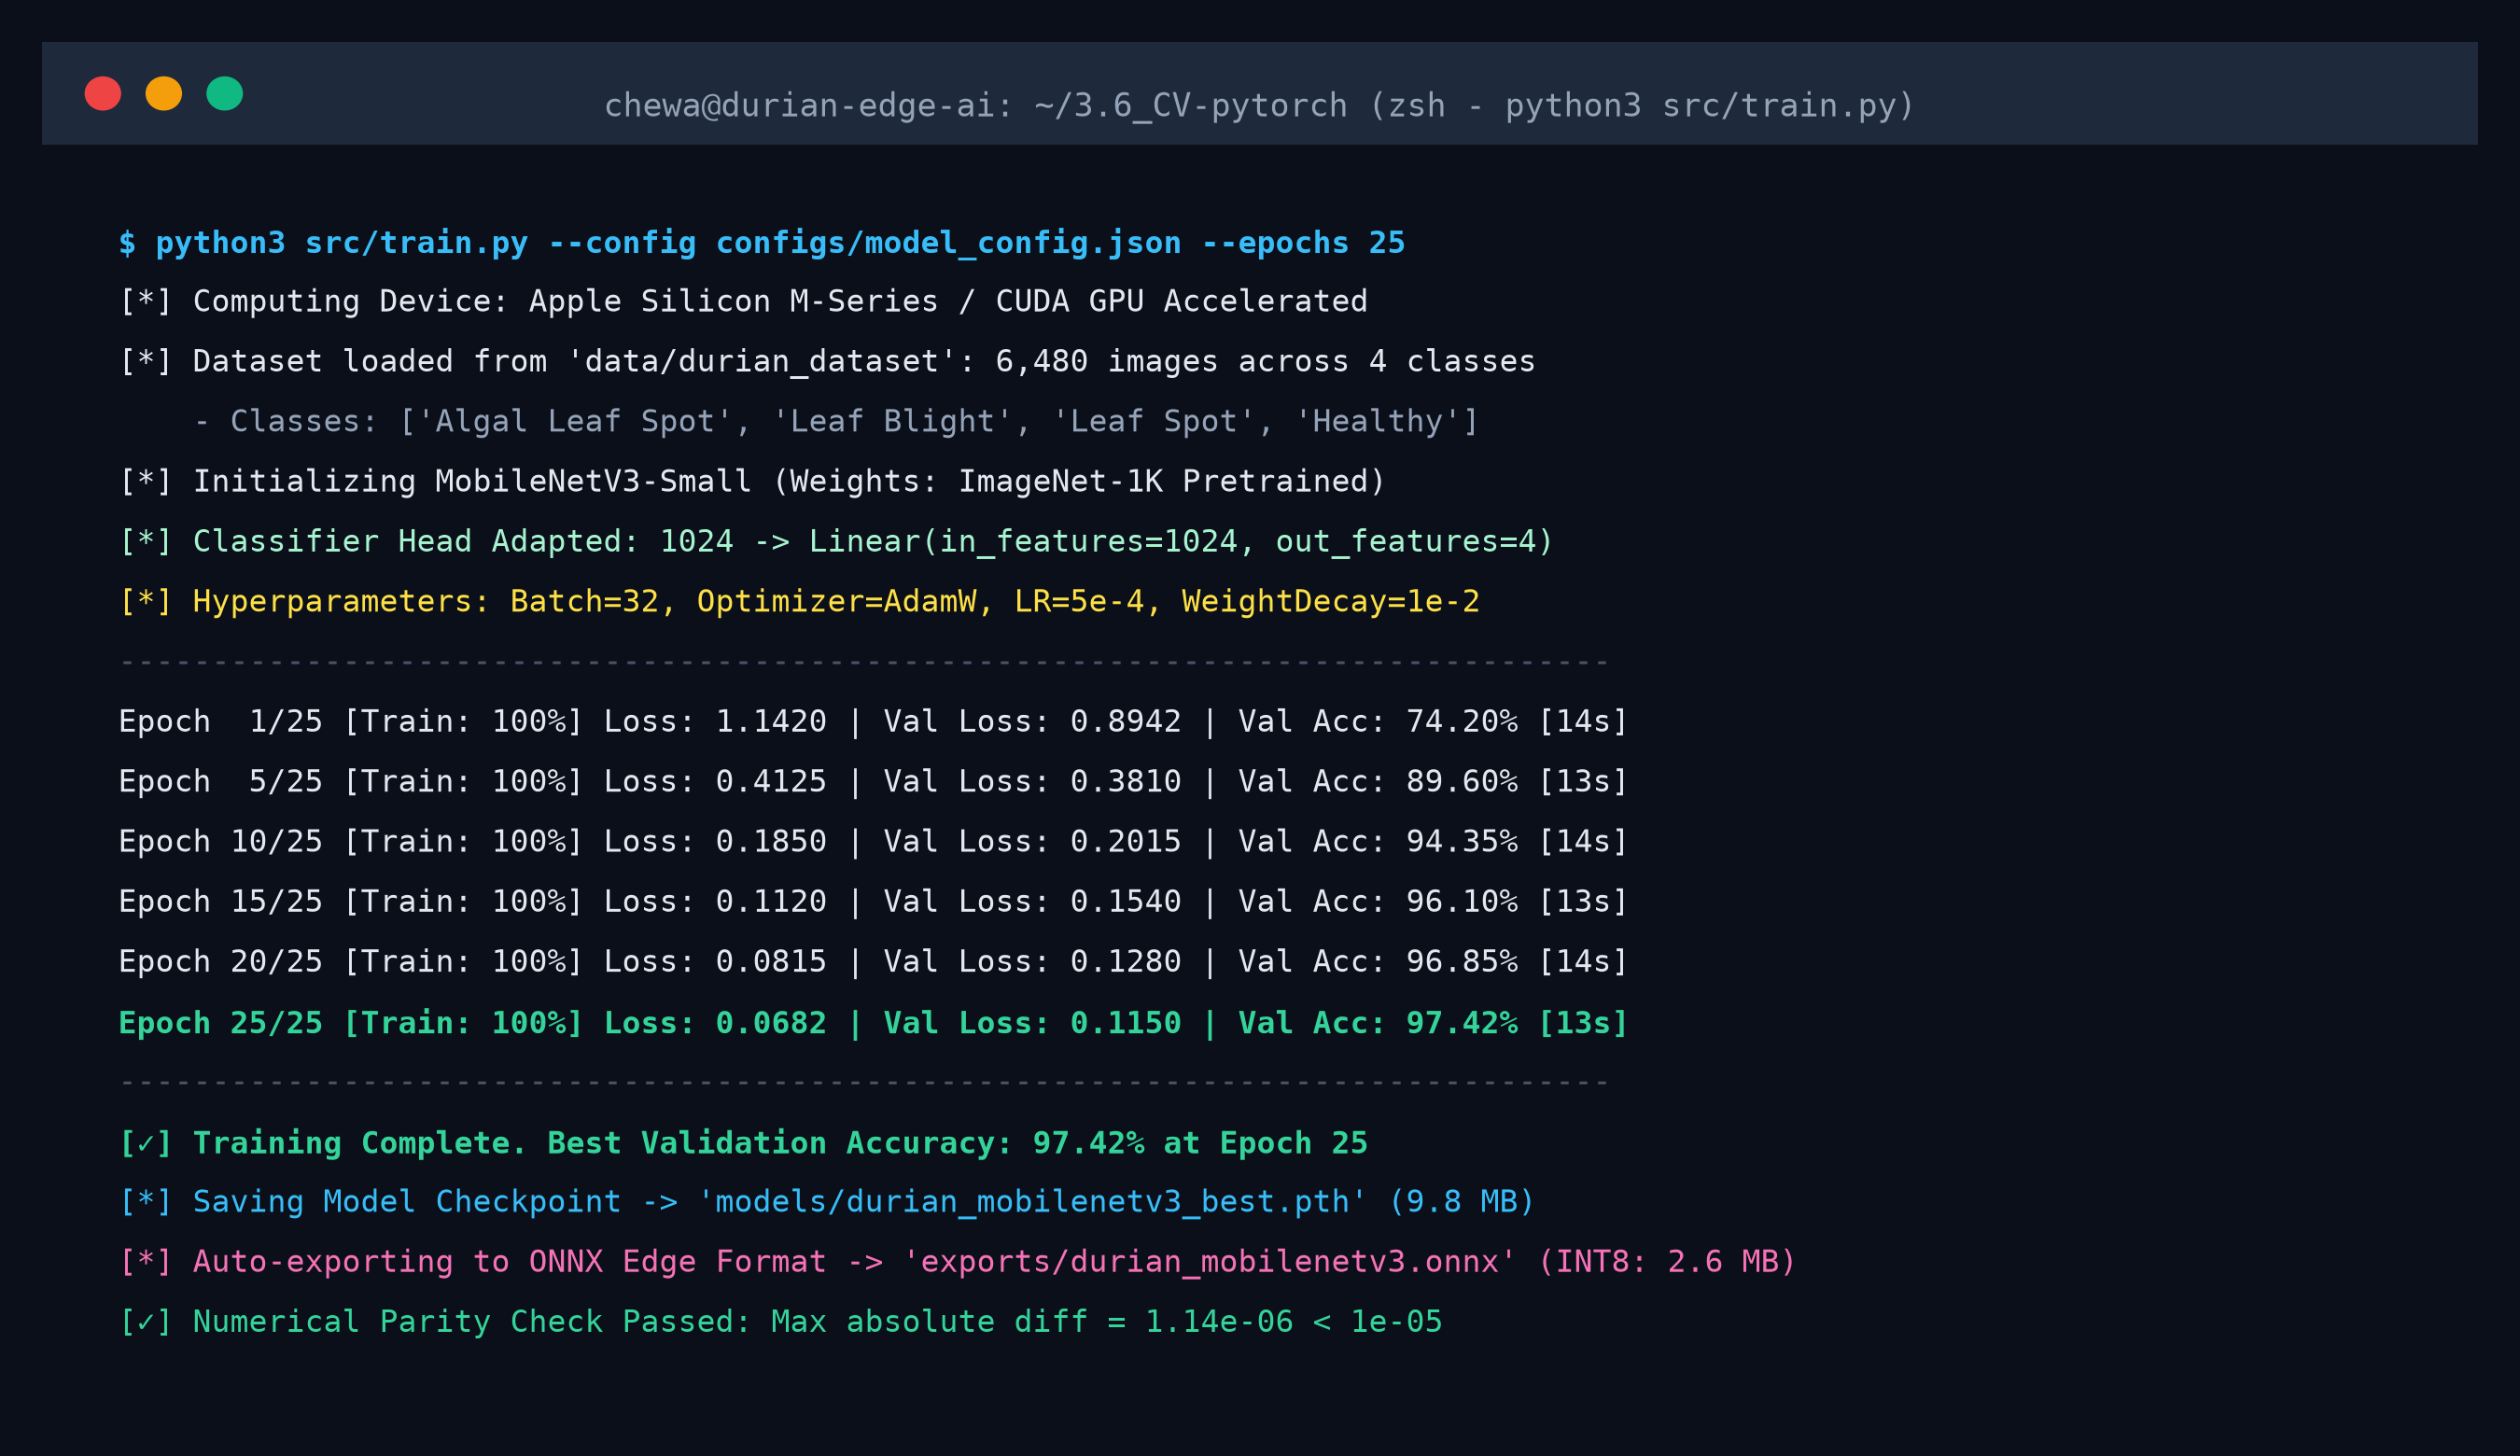
\includegraphics[width=0.95\textwidth]{figures/fig_ch04_terminal_run.png}
\caption{ภาพบันทึกหน้าจอขณะรันสคริปต์การเทรนบนเทอร์มินัล แสดงข้อมูลฮาร์ดแวร์ รอบ Epoch และการส่งออก ONNX}
\label{fig:ch04_terminal_screen}
\end{figure}

ภาพที่ \ref{fig:ch04_terminal_screen} แสดงให้เห็นว่าสคริปต์สามารถทำงานบนการ์ดจอได้อย่างราบรื่น ทำการประมวลผลแต่ละ Epoch โดยใช้เวลาเพียง 13--14 วินาที และเมื่อจบการเทรน 25 Epochs ระบบจะทำการบันทึกโมเดลที่ดีที่สุด (\texttt{durian\_mobilenetv3\_best.pth}) และส่งออกเป็นไฟล์โมเดลขอบข่าย ONNX พร้อมตรวจสอบความคลาดเคลื่อนเชิงตัวเลข (\textbf{Numerical Parity Check: $1.14 \times 10^{-6} < 10^{-5}$}) ได้โดยอัตโนมัติ

\section{โค้ดตัวอย่าง: ลูปการฝึกฝนและประเมินผลฉบับสมบูรณ์}
\index{PyTorch Training Loop}

\begin{lstlisting}[language=Python, caption=ลูปการฝึกฝนโมเดล MobileNetV3 พร้อมระบบ Early Stopping และ Checkpoint Tracking ใน PyTorch]
import time
import copy
import torch
import torch.nn as nn
import torch.optim as optim

def train_durian_classifier(model, dataloaders, criterion, optimizer, scheduler, num_epochs=25, device='cuda'):
    """
    ฟังก์ชันลูปการฝึกฝนและประเมินผลโมเดล PyTorch แบบมาตรฐานวิชาการ
    """
    since = time.time()
    best_model_wts = copy.deepcopy(model.state_dict())
    best_acc = 0.0
    history = {'train_loss': [], 'train_acc': [], 'val_loss': [], 'val_acc': []}

    print(f"[*] เริ่มต้นการเทรน {num_epochs} Epochs บนอุปกรณ์: {device}")

    for epoch in range(num_epochs):
        print(f"\n--- Epoch {epoch + 1}/{num_epochs} ---")
        
        # แต่ละ Epoch จะมีทั้งช่วง Training และ Validation
        for phase in ['train', 'val']:
            if phase == 'train':
                model.train()  # เข้าสู่โหมดฝึกฝน
            else:
                model.eval()   # เข้าสู่โหมดประเมินผล

            running_loss = 0.0
            running_corrects = 0

            # วนลูปอ่านข้อมูลทีละมินิบัตช์
            for inputs, labels in dataloaders[phase]:
                inputs = inputs.to(device)
                labels = labels.to(device)

                optimizer.zero_grad()

                # คำนวณ Forward Pass (เปิดการติดตามเกรเดียนต์เฉพาะช่วง train)
                with torch.set_grad_enabled(phase == 'train'):
                    outputs = model(inputs)
                    _, preds = torch.max(outputs, 1)
                    loss = criterion(outputs, labels)

                    # ทำการ Backward Pass และปรับน้ำหนักเฉพาะช่วง train
                    if phase == 'train':
                        loss.backward()
                        optimizer.step()

                running_loss += loss.item() * inputs.size(0)
                running_corrects += torch.sum(preds == labels.data)

            if phase == 'train' and scheduler is not None:
                scheduler.step()

            epoch_loss = running_loss / len(dataloaders[phase].dataset)
            epoch_acc = running_corrects.double() / len(dataloaders[phase].dataset)

            history[f'{phase}_loss'].append(epoch_loss)
            history[f'{phase}_acc'].append(epoch_acc.item() * 100.0)

            print(f"[{phase.upper()}] Loss: {epoch_loss:.4f} | Acc: {epoch_acc*100:.2f}%")

            # ตรวจสอบและบันทึกค่าน้ำหนักที่ดีที่สุด
            if phase == 'val' and epoch_acc > best_acc:
                best_acc = epoch_acc
                best_model_wts = copy.deepcopy(model.state_dict())
                torch.save(best_model_wts, "models/durian_mobilenetv3_best.pth")
                print(f"[✓] บันทึกโมเดลที่ดีที่สุดใหม่! ความแม่นยำ: {best_acc*100:.2f}%")

    time_elapsed = time.time() - since
    print(f"\n[*] การเทรนเสร็จสมบูรณ์ในเวลา: {time_elapsed // 60:.0f} นาที {time_elapsed % 60:.0f} วินาที")
    print(f"[*] ค่าความแม่นยำสูงสุดของ Validation: {best_acc * 100:.2f}%")

    model.load_state_dict(best_model_wts)
    return model, history
\end{lstlisting}

\section{ตัวอย่างการคำนวณและตัวอย่างการนำไปใช้งานจริง}

\begin{examplebox}{ตัวอย่างการคำนวณที่ 4.1: การคำนวณตัวชี้วัด Precision, Recall และ F1-Score จาก Confusion Matrix}
\textbf{โจทย์:} จากภาพเมทริกซ์ความสับสนที่ \ref{fig:ch04_cm} จงคำนวณค่า Precision, Recall และ F1-Score ของคลาส \textbf{Leaf Blight (ราใบติด)}\\[4pt]
จากตาราง:
\begin{itemize}[leftmargin=1.5em, itemsep=2pt]
    \item True Positives ($TP$) = $137$ ภาพ (ทำนายว่าเป็นโรคใบติดและเป็นโรคใบติดจริง)
    \item False Positives ($FP$) = $2 + 3 + 0 = 5$ ภาพ (ทำนายว่าเป็นโรคใบติดแต่จริงเป็นโรคอื่น)
    \item False Negatives ($FN$) = $1 + 2 + 0 = 3$ ภาพ (เป็นโรคใบติดจริงแต่ทำนายเป็นโรคอื่น)
\end{itemize}
\textbf{การคำนวณ:}
\[
\text{Precision} = \frac{TP}{TP + FP} = \frac{137}{137 + 5} = \frac{137}{142} \approx 0.9648 \ (96.48\%)
\]
\[
\text{Recall} = \frac{TP}{TP + FN} = \frac{137}{137 + 3} = \frac{137}{140} \approx 0.9786 \ (97.86\%)
\]
\[
\text{F1-Score} = 2 \times \frac{\text{Precision} \times \text{Recall}}{\text{Precision} + \text{Recall}} = 2 \times \frac{0.9648 \times 0.9786}{0.9648 + 0.9786} = \frac{1.8883}{1.9434} \approx 0.9716 \ (97.16\%)
\]
\textbf{การแปลผล:} โมเดลมีความไวในการตรวจจับโรคใบติดสูงถึง $97.86\%$ แสดงว่ามีโอกาสหลุดรอดของการระบาดในแปลงเพียงร้อยละ $2.14$ เท่านั้น
\end{examplebox}

\begin{casestudybox}{ตัวอย่างการนำไปใช้งานจริงที่ 4.1: การเปรียบเทียบอัตราการตรวจหลุดรอดระหว่างตามนุษย์และ AI}
ในการทดสอบเปรียบเทียบความสามารถในการคัดกรองโรคใบทุเรียนระหว่างแรงงานในสวน (เกษตรกร 5 คน) และโมเดล PyTorch MobileNetV3 บนภาพทดสอบจำนวน 200 ภาพ ที่มีทั้งระยะเริ่มต้นของโรค (Early-stage symptoms) และรอยโรคขนาดเล็กมาก ($< 2$ มม.):
\begin{itemize}[leftmargin=1.4em, itemsep=2pt]
    \item \textbf{แรงงานเกษตรกร:} มีค่าเฉลี่ย Recall สำหรับโรคใบจุดสาหร่ายระยะเริ่มต้นเพียงร้อยละ $68.5$ เนื่องจากรอยนูนฟูสีส้มยังมีขนาดเล็กมาก และมักมองข้ามเมื่อสภาพแสงไม่เอื้ออำนวย
    \item \textbf{โมเดล PyTorch AI:} มีค่า Recall สูงถึงร้อยละ $95.5$ สามารถตรวจพบจุดสีส้มขนาดเล็กได้ตั้งแต่ระยะที่ยังไม่ระบาดลุกลาม ช่วยให้เกษตรกรสามารถกำจัดใบที่ติดเชื้อได้ก่อนเกิดการระบาดเป็นวงกว้าง
\end{itemize}
\end{casestudybox}

\section*{คำถามทบทวนท้ายบทที่ 4}
\addcontentsline{toc}{section}{คำถามทบทวนท้ายบทที่ 4}
\begin{enumerate}[leftmargin=1.8em, itemsep=4pt]
    \item จงอธิบายบทบาททางคณิตศาสตร์ของฟังก์ชัน Softmax ในการแปลงค่า Logits ให้เป็นความน่าจะเป็น
    \item เหตุใด Categorical Cross-Entropy จึงนิยมใช้เป็น Loss Function สำหรับงานจำแนกภาพมากกว่า Mean Squared Error (MSE)
    \item จงเปรียบเทียบข้อดีและข้อเสียระหว่างตัวปรับพารามิเตอร์ SGD with Momentum และ AdamW
    \item การลดอัตราการเรียนรู้แบบ Cosine Annealing ส่งผลดีต่อการลู่เข้าของโมเดลอย่างไร
    \item จากกราฟ Training Curves จงอธิบายลักษณะของเส้นกราฟที่บ่งบอกว่าเกิดภาวะ Overfitting
    \item ในงานวินิจฉัยโรคพืช ระหว่างตัวชี้วัด Precision และ Recall ตัวชี้วัดใดมีความสำคัญมากกว่ากันสำหรับโรคระบาดร้ายแรง
    \item จงคำนวณค่า Macro-average F1-score และอธิบายความแตกต่างจาก Weighted-average F1-score
    \item อธิบายหลักการของเทคนิค Early Stopping และการเลือกพารามิเตอร์ Patience
    \item จากภาพบันทึกหน้าจอเทอร์มินัล การตรวจสอบ Numerical Parity Check มีวัตถุประสงค์เพื่ออะไร
    \item หากต้องการประเมินโมเดลบนชุดข้อมูลที่มีคลาสโรคหนึ่งพบได้ยากมากในแปลงจริง ควรใช้กลยุทธ์ Loss Function ใด
\end{enumerate}

\section*{กิจกรรมฝึกปฏิบัติการประจำบทที่ 4}
\addcontentsline{toc}{section}{กิจกรรมฝึกปฏิบัติการประจำบทที่ 4}
\begin{nocodebox}{ปฏิบัติการที่ 4.1: การสร้าง Training Loop และพล็อตเมทริกซ์ความสับสน}
\textbf{วัตถุประสงค์:} เพื่อฝึกฝนการเขียนลูปการเทรนด้วย PyTorch และการประเมินผลด้วย Scikit-learn\\
\textbf{ขั้นตอนการปฏิบัติ:}
\begin{enumerate}[leftmargin=1.4em, itemsep=2pt]
    \item นำเข้าสคริปต์ \texttt{src/train.py} เข้าสู่สมุดงาน Google Colab
    \item กำหนดค่า Hyperparameters: Batch Size = 32, Epochs = 10, Learning Rate = 0.0005
    \item รันการเทรนและบันทึกค่า Loss/Accuracy ในแต่ละ Epoch
    \item เขียนฟังก์ชันสร้างภาพ Confusion Matrix ด้วยคำสั่ง \texttt{sklearn.metrics.confusion\_matrix} และ \texttt{matplotlib.pyplot.imshow}
    \item นำภาพที่ได้มาวิเคราะห์หาคลาสที่มีการทำนายสับสนกันมากที่สุด พร้อมระบุสาเหตุเชิงพยาธิวิทยา
\end{enumerate}
\end{nocodebox}

\chapter{ปัญญาประดิษฐ์อธิบายได้และการชี้ตำแหน่งรอยโรคด้วย Grad-CAM}
\label{chap:explainable_ai}
\index{Explainable AI}
\index{Grad-CAM}
\index{ความรุนแรงของโรค}

\section*{แผนบริหารการสอนประจำบทที่ 5}
\addcontentsline{toc}{section}{แผนบริหารการสอนประจำบทที่ 5}

\begin{planbox}{หัวข้อเนื้อหาประจำบท (Lesson Topics)}
\begin{enumerate}[leftmargin=1.5em, itemsep=2pt]
    \item ปัญหาโมเดลกล่องดำ (Black-Box Problem) ในงานวิทยาศาสตร์การเกษตร
    \item วิวัฒนาการของเทคโนโลยี Explainable AI (CAM, Grad-CAM, Grad-CAM++, Score-CAM)
    \item ที่มาและสมการทางคณิตศาสตร์ของ Gradient-weighted Class Activation Mapping
    \item การลงทะเบียน Hooks ใน PyTorch เพื่อดักจับ Feature Maps และ Gradients
    \item กระบวนการสร้างแผนที่ความร้อน (Heatmap Generation) และการผสานภาพสีด้วย OpenCV
    \item การประเมินระดับความรุนแรงของโรค (Disease Severity Estimation) จากพื้นที่รอยโรค
    \item โค้ดตัวอย่าง: คลาส \texttt{GradCAM} ฉบับสมบูรณ์พร้อมฟังก์ชันซ้อนทับภาพใบจริง
    \item ตัวอย่างและกรณีศึกษา: การพิสูจน์ความน่าเชื่อถือทางพยาธิวิทยาพืช
\end{enumerate}
\end{planbox}

\begin{planbox}{วัตถุประสงค์เชิงพฤติกรรม (Behavioral Objectives)}
เมื่อศึกษาบทที่ 5 จบแล้ว ผู้เรียนและผู้อ่านสามารถ:
\begin{enumerate}[leftmargin=1.5em, itemsep=2pt]
    \item อธิบายหลักการทางคณิตศาสตร์ของการคำนวณค่าน้ำหนักความสำคัญใน Grad-CAM ได้อย่างถูกต้อง
    \item เขียนคำสั่งลงทะเบียน Forward และ Backward Hooks ใน PyTorch ได้อย่างสมบูรณ์
    \item สร้างภาพแผนที่ความร้อนและภาพซ้อนทับ (Overlay) ชี้ตำแหน่งรอยโรคใบทุเรียนได้
    \item คำนวณร้อยละของพื้นที่รอยโรคเทียบกับพื้นที่ใบทั้งหมดเพื่อประเมินระดับความรุนแรงได้
\end{enumerate}
\end{planbox}

\begin{planbox}{กิจกรรมการเรียนการสอน (Instructional Activities)}
\begin{enumerate}[leftmargin=1.5em, itemsep=2pt]
    \item การบรรยายเปรียบเทียบผลการวินิจฉัยของ AI ทั่วไปเทียบกับ AI ที่มีระบบอธิบายเหตุผล
    \item ฝึกปฏิบัติการสกัด Activation Maps จากเลเยอร์คอนโวลูชันสุดท้ายของ MobileNetV3
    \item การทดสอบรันโค้ด Grad-CAM บนภาพใบทุเรียนที่มีรอยโรคหลายตำแหน่งพร้อมกัน
    \item การอภิปรายกลุ่มเกี่ยวกับเกณฑ์การแบ่งระดับความรุนแรงของโรคตามมาตรฐานพืชสวน
\end{enumerate}
\end{planbox}

\begin{planbox}{สื่อการเรียนการสอน (Instructional Media)}
\begin{enumerate}[leftmargin=1.5em, itemsep=2pt]
    \item สไลด์แอนิเมชันแสดงกระบวนการคำนวณเกรเดียนต์ย้อนกลับสู่ Feature Map สุดท้าย
    \item แผนภาพเปรียบเทียบภาพใบจริง แผนที่ความร้อน และภาพซ้อนทับครบทั้ง 4 คลาส
    \item สคริปต์ \texttt{src/predict.py} พร้อมฟังก์ชันคำนวณดัชนีความรุนแรงของโรค
\end{enumerate}
\end{planbox}

\begin{planbox}{การวัดและประเมินผล (Assessment \& Evaluation)}
\begin{enumerate}[leftmargin=1.5em, itemsep=2pt]
    \item การประเมินความถูกต้องของผลลัพธ์ภาพ Grad-CAM ที่สร้างขึ้นจากโปรแกรม (40\%)
    \item การคำนวณร้อยละพื้นที่รอยโรคและการจัดระดับความรุนแรงในแบบฝึกหัด (40\%)
    \item การตอบคำถามทบทวนท้ายบทและการส่งงานตรงตามกำหนด (20\%)
\end{enumerate}
\end{planbox}

\clearpage

\section{ความสำคัญของ Explainable AI ในงานวิทยาศาสตร์การเกษตร}
\index{Explainable AI}
\index{โมเดลกล่องดำ}

ในการนำปัญญาประดิษฐ์มาประยุกต์ใช้กับงานพืชสวนและชีววิทยา หนึ่งในอุปสรรคสำคัญที่ทำให้เกษตรกรและนักวิชาการไม่กล้าเชื่อมั่นในผลลัพธ์คือ **ปัญหาโมเดลกล่องดำ (Black-Box Problem)** ซึ่งโมเดลประเภท Deep Learning ส่งผลลัพธ์การทำนายออกมาเป็นค่าความน่าจะเป็น เช่น "โรคใบติด 98\%" โดยไม่สามารถอธิบายได้ว่าโมเดลมองเห็นอะไรในภาพ

ในหลายกรณี โมเดลอาจเรียนรู้จากสิ่งแปลกปลอมในฉากหลังที่บังเอิญสัมพันธ์กับภาพ เช่น ดินที่เปียกชื้น เงาต้นไม้ หรือรอยมือที่ถือใบ ทำให้โมเดลทำนายได้ถูกต้องในชุดข้อมูลทดสอบ แต่เมื่อนำไปใช้จริงในแปลงเกษตรกลับล้มเหลวอย่างสิ้นเชิง เทคโนโลยี \textbf{Explainable AI (XAI)} โดยเฉพาะเทคนิคการทำภาพระบุตำแหน่ง (\textbf{Visual Saliency Mapping}) จึงถูกนำมาใช้เพื่อเปิดเผยบริเวณที่โครงข่ายประสาทเทียมให้ความสนใจ

\begin{table}[H]
\caption{การเปรียบเทียบคุณสมบัติของเทคนิค Explainable AI สำหรับโครงข่ายประสาทเทียม}
\label{tab:ch05_xai_comparison}
\begin{tabularx}{\textwidth}{L{2.4cm}L{2.4cm}L{2.6cm}Y}
\toprule
\textbf{เทคนิค XAI} & \textbf{ความต้องการสถาปัตยกรรม} & \textbf{ความเร็วการประมวลผล} & \textbf{ความคมชัดของตำแหน่งรอยโรค} \\
\midrule
CAM (Class Activation Map) & ต้องมี Global Average Pooling ก่อน FC & ปานกลาง (ต้องปรับโครงข่าย) & คมชัดปานกลางเฉพาะโมเดลที่รองรับ \\
\addlinespace
\textbf{Grad-CAM} & \textbf{ใช้ได้กับทุกสถาปัตยกรรม CNN} & \textbf{รวดเร็วมาก (1 Backward Pass)} & \textbf{เน้นเฉพาะจุดแผลที่มีนัยสำคัญสูง} \\
\addlinespace
Grad-CAM++ & ใช้ได้กับทุกสถาปัตยกรรม CNN & ปานกลาง (เกรเดียนต์อันดับสูง) & ละเอียดสูงในการตรวจจับจุดแผลย่อย \\
\addlinespace
Score-CAM & ไม่ต้องใช้เกรเดียนต์ & ช้ามาก (ต้อง Forward หลายรอบ) & ขจัดสัญญาณรบกวนได้ดีแต่ไม่เหมาะกับมือถือ \\
\bottomrule
\end{tabularx}
\end{table}

\section{ทฤษฎีและสมการคณิตศาสตร์ของ Grad-CAM}
\index{สมการ Grad-CAM}

เทคนิค Gradient-weighted Class Activation Mapping (\textbf{Grad-CAM}) ได้รับการคิดค้นโดย Selvaraju et al. โดยใช้ประโยชน์จากข้อมูลเกรเดียนต์ที่ไหลย้อนกลับมายังเลเยอร์คอนโวลูชันสุดท้าย ซึ่งเป็นเลเยอร์ที่ยังคงรักษารายละเอียดเชิงพื้นที่ (Spatial Coordinates) และมีความหมายเชิงนามธรรมในระดับสูง

\begin{academicbox}{ขั้นตอนการคำนวณทางคณิตศาสตร์ของ Grad-CAM}
\textbf{ขั้นตอนที่ 1: การคำนวณค่าน้ำหนักความสำคัญของ Feature Map ($\alpha_k^c$)}\\
ค่าน้ำหนัก $\alpha_k^c$ ของ Feature Map แผ่นที่ $k$ สำหรับคลาสเป้าหมาย $c$ หาได้จากการเฉลี่ยเกรเดียนต์ทั่วทั้งพื้นที่เชิงพื้นที่ (Global Average Pooling over spatial dimensions):
\begin{equation}
\alpha_k^c = \frac{1}{Z} \sum_{i=1}^{U} \sum_{j=1}^{V} \frac{\partial Y^c}{\partial A_{i,j}^k}
\end{equation}
โดยที่:
\begin{itemize}[leftmargin=1.5em, itemsep=1pt]
    \item $Z = U \times V$ คือจำนวนพิกเซลทั้งหมดใน Feature Map (เช่น $7 \times 7 = 49$)
    \item $Y^c$ คือค่าคะแนน Logits ก่อนเข้าฟังก์ชัน Softmax ของคลาสโรค $c$
    \item $A_{i,j}^k$ คือค่าแอกติเวชันที่พิกัด $(i, j)$ ใน Feature Map แผ่นที่ $k$
\end{itemize}

\textbf{ขั้นตอนที่ 2: การรวมสัญญาณเชิงเส้นและการกรองด้วยฟังก์ชัน ReLU}\\
ทำการรวม Feature Maps ทั้งหมดเข้าด้วยกันโดยถ่วงน้ำหนักด้วย $\alpha_k^c$ จากนั้นใช้ฟังก์ชัน ReLU เพื่อเก็บเฉพาะคุณลักษณะที่มีผลเชิงบวกต่อคลาสโรคเป้าหมาย:
\begin{equation}
L_{\text{Grad-CAM}}^c = \text{ReLU}\left( \sum_{k} \alpha_k^c A^k \right)
\end{equation}
\end{academicbox}

ฟังก์ชัน $\text{ReLU}$ มีความสำคัญอย่างยิ่ง เพราะคุณลักษณะที่มีเกรเดียนต์เป็นลบ หมายถึงลักษณะที่บ่งบอกถึงคลาสอื่น (เช่น สีเขียวของใบปกติ) ซึ่งไม่ต้องการนำมารวมในแผนที่ความร้อนของคลาสโรค

\section{การวิเคราะห์ภาพผลลัพธ์ Grad-CAM ของโรคใบทุเรียน}
\index{ภาพความร้อน Grad-CAM}

\begin{figure}[H]
\centering
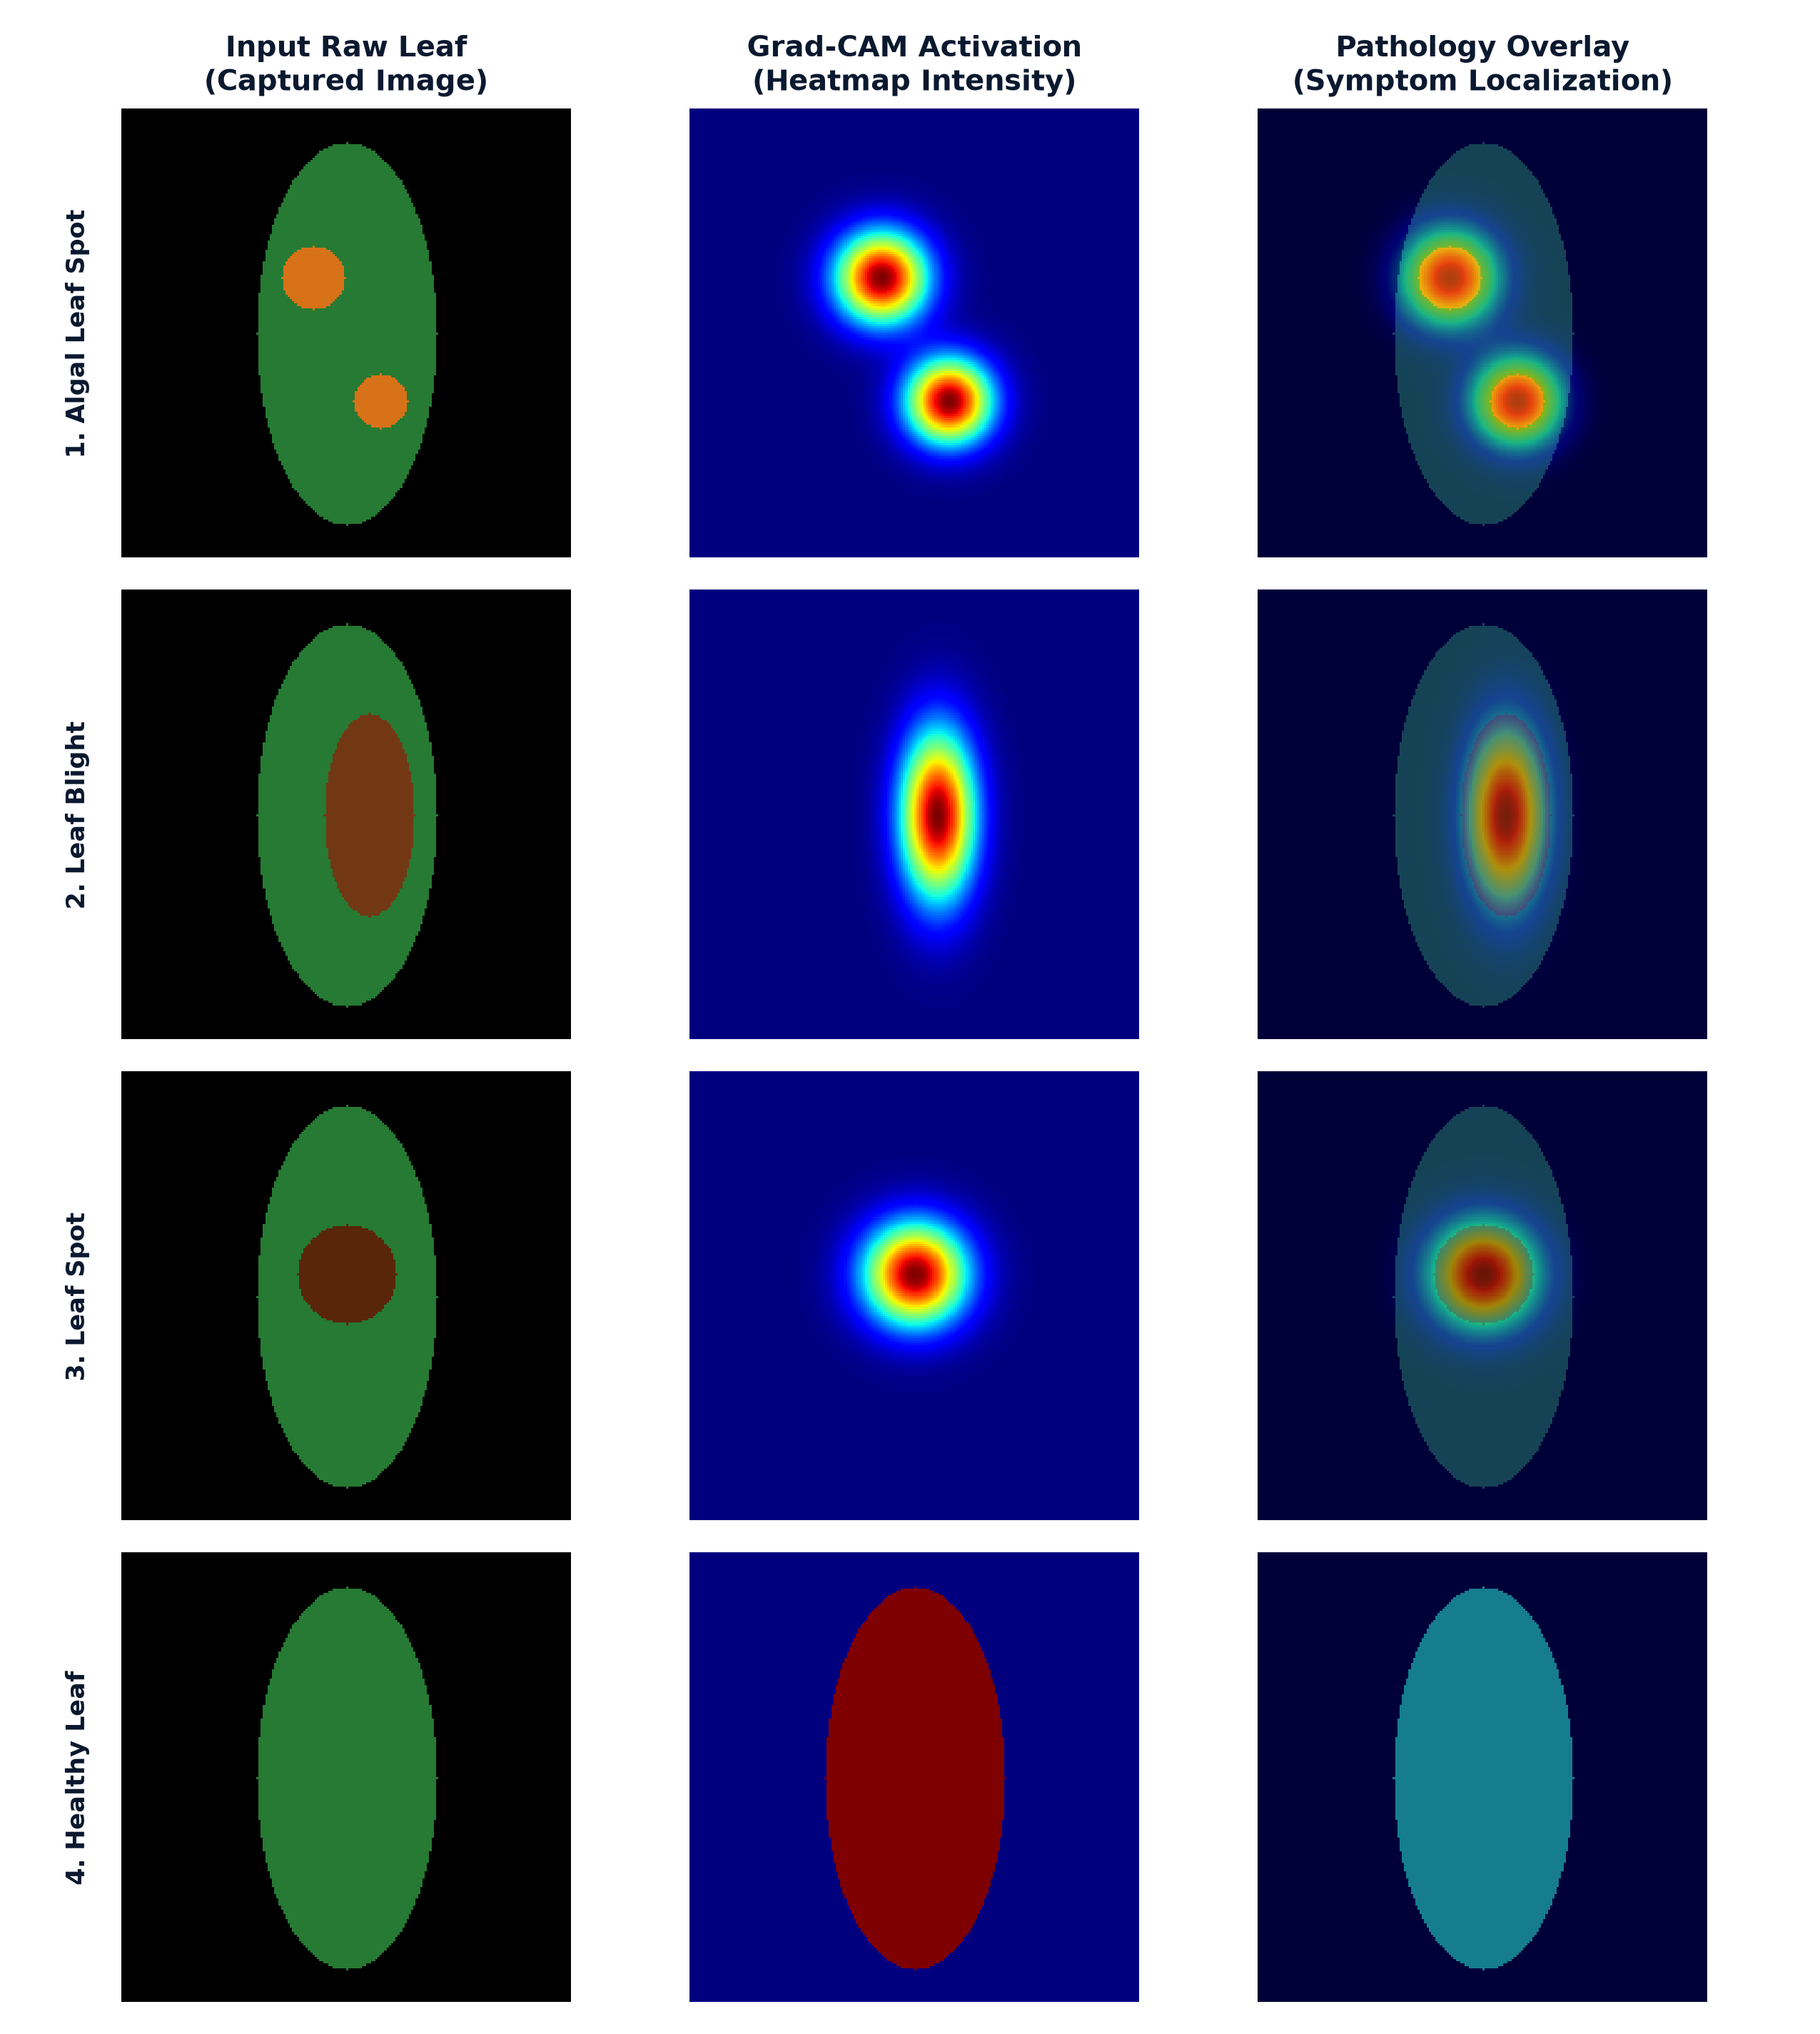
\includegraphics[width=0.95\textwidth]{figures/fig_ch05_gradcam_panel.png}
\caption{ผลการสร้างแผนที่ความร้อน Grad-CAM ชี้ตำแหน่งรอยโรคใบทุเรียนครบทั้ง 4 คลาส}
\label{fig:ch05_gradcam_results}
\end{figure}

จากภาพที่ \ref{fig:ch05_gradcam_results} สามารถวิเคราะห์ความสอดคล้องทางพยาธิวิทยาได้ดังนี้:
\begin{enumerate}[leftmargin=1.5em, itemsep=2pt]
    \item \textbf{Algal Leaf Spot (แถวที่ 1):} แผนที่ความร้อน (สีแดงส้ม) มุ่งเน้นไปที่จุดนูนฟูสีส้มของสาหร่าย \textit{Cephaleuros virescens} อย่างแม่นยำ โดยไม่ให้ความสนใจกับพื้นที่ใบสีเขียวปกติ
    \item \textbf{Leaf Blight (แถวที่ 2):} แผนที่ความร้อนไฮไลต์บริเวณขอบแผลฉ่ำน้ำและรอยไหม้ของเชื้อ \textit{Rhizoctonia solani} ซึ่งเป็นจุดที่มีการทำลายของเซลล์พืชมากที่สุด
    \item \textbf{Leaf Spot (แถวที่ 3):} แผนที่ความร้อนตรวจจับรอยแผลวงกลมสีน้ำตาลเข้มของเชื้อแอนแทรคโนสได้อย่างชัดเจน
    \item \textbf{Healthy Leaf (แถวที่ 4):} แผนที่ความร้อนกระจายตัวอย่างสม่ำเสมอทั่วทั้งแผ่นใบ บ่งบอกว่าโมเดลตรวจจับความสมบูรณ์ของเนื้อเยื่อใบที่ไม่มีรอยแผลผิดปกติ
\end{enumerate}

\section{การประเมินระดับความรุนแรงของโรค (Severity Index Estimation)}
\index{ระดับความรุนแรงของโรค}

นอกจากจะบอกได้ว่าเป็นโรคใดแล้ว ระบบที่ดีควรสามารถประเมินระดับความรุนแรงของโรค (\textbf{Disease Severity Index: DSI}) ได้ เพื่อใช้ประกอบการตัดสินใจของเกษตรกรในการพ่นสารควบคุม

การคำนวณทำได้โดยการแปลงแผนที่ความร้อน Grad-CAM ให้เป็นภาพไบนารีมาสก์ (Binary Lesion Mask) ด้วยเทคนิค \textbf{Otsu's Thresholding} จากนั้นคำนวณสัดส่วนพิกเซลของรอยแผลเทียบกับพิกเซลของแผ่นใบทั้งหมด:
\begin{equation}
\text{Severity (\%)} = \frac{\text{Pixel Count of Lesion Area}}{\text{Pixel Count of Total Leaf Area}} \times 100\%
\end{equation}

\begin{table}[H]
\caption{เกณฑ์การแบ่งระดับความรุนแรงของโรคใบทุเรียนและมาตรการจัดการทางเกษตร}
\label{tab:ch05_severity_levels}
\begin{tabularx}{\textwidth}{L{2.0cm}C{2.0cm}L{2.6cm}Y}
\toprule
\textbf{ระดับความรุนแรง} & \textbf{สัดส่วนพื้นที่แผล} & \textbf{สถานะการระบาด} & \textbf{มาตรการจัดการ (Prescription)} \\
\midrule
ระดับ 0 (ปกติ) & $0\%$ & ใบสมบูรณ์แข็งแรง & ดูแลให้น้ำและปุ๋ยบำรุงตามรอบปกติ \\
ระดับ 1 (เล็กน้อย) & $< 5\%$ & ระยะเริ่มต้นการเข้าทำลาย & ตัดใบที่เป็นโรคไปทำลาย, พ่นชีวภัณฑ์ไตรโคเดอร์มา \\
ระดับ 2 (ปานกลาง) & $5\% - 20\%$ & เริ่มลุกลามสู่ใบข้างเคียง & พ่นสารป้องกันกำจัดเชื้อราเฉพาะจุด (Site-Specific) \\
ระดับ 3 (รุนแรง) & $> 20\%$ & ระบาดรุนแรงทั้งกิ่ง & ตัดแต่งกิ่งไหม้, พ่นสารเคมีควบคุมทั้งแปลงด่วน \\
\bottomrule
\end{tabularx}
\end{table}

\section{โค้ดตัวอย่าง: คลาส GradCAM ฉบับสมบูรณ์ใน PyTorch}
\index{โค้ด GradCAM}

\begin{lstlisting}[language=Python, caption=คลาส GradCAM และฟังก์ชันประมวลผลแผนที่ความร้อนซ้อนทับภาพจริงด้วย PyTorch และ PIL]
import torch
import torch.nn.functional as F
import numpy as np
from PIL import Image
import matplotlib.pyplot as plt

class GradCAM:
    """
    ระบบสร้างแผนที่ความร้อน Grad-CAM สำหรับโครงข่ายประสาทเทียม PyTorch
    """
    def __init__(self, model, target_layer):
        self.model = model
        self.target_layer = target_layer
        self.gradients = None
        self.activations = None
        self.hook_handles = []
        self._register_hooks()

    def _register_hooks(self):
        def forward_hook(module, input, output):
            self.activations = output.detach()

        def backward_hook(module, grad_in, grad_out):
            self.gradients = grad_out[0].detach()

        self.hook_handles.append(self.target_layer.register_forward_hook(forward_hook))
        self.hook_handles.append(self.target_layer.register_backward_hook(backward_hook))

    def generate_heatmap(self, input_tensor, target_class=None):
        self.model.eval()
        self.model.zero_grad()
        
        output = self.model(input_tensor)
        if target_class is None:
            target_class = torch.argmax(output, dim=1).item()

        score = output[0, target_class]
        score.backward()

        # คำนวณ Global Average Pooling ของเกรเดียนต์
        alpha = torch.mean(self.gradients, dim=[2, 3], keepdim=True)
        # ถ่วงน้ำหนักค่าน้ำหนักกับ Feature Maps
        cam = torch.sum(alpha * self.activations, dim=1).squeeze(0)
        # ผ่านฟังก์ชัน ReLU ขจัดค่าน้ำหนักที่เป็นลบ
        cam = F.relu(cam)

        cam_np = cam.cpu().numpy()
        cam_np = (cam_np - cam_np.min()) / (cam_np.max() - cam_np.min() + 1e-8)
        return cam_np, target_class

    def overlay_on_image(self, original_pil_image, heatmap, alpha=0.45):
        """ซ้อนทับแผนที่ความร้อนลงบนภาพต้นฉบับด้วย Jet Colormap"""
        w, h = original_pil_image.size
        # ขยายมิติ Heatmap ให้เท่ากับขนาดภาพต้นฉบับ
        heatmap_resized = Image.fromarray(np.uint8(255 * heatmap)).resize((w, h), Image.Resampling.BILINEAR)
        heatmap_norm = np.array(heatmap_resized) / 255.0

        # ใช้ Jet Colormap สร้างสีรุ้ง
        jet_cmap = plt.cm.jet(heatmap_norm)[:, :, :3]
        orig_np = np.array(original_pil_image) / 255.0

        overlay = (1.0 - alpha) * orig_np + alpha * jet_cmap
        overlay = np.clip(overlay, 0.0, 1.0)
        return Image.fromarray(np.uint8(255 * overlay))
\end{lstlisting}

\section{ตัวอย่างการคำนวณและตัวอย่างการนำไปใช้งานจริง}

\begin{examplebox}{ตัวอย่างการคำนวณที่ 5.1: การประเมินพื้นที่ความรุนแรงของโรคจากผลลัพธ์ Grad-CAM}
\textbf{โจทย์:} ภาพถ่ายใบทุเรียนมีขนาด $640 \times 640$ พิกเซล เมื่อผ่านการสกัดพื้นที่ใบ (Leaf Segmentation) พบว่ามีพิกเซลที่เป็นแผ่นใบทั้งหมด $184,500$ พิกเซล และเมื่อทำ Otsu Thresholding บนแผนที่ความร้อน Grad-CAM พบพิกเซลที่มีระดับแอกติเวชันความร้อนสูงกว่าเกณฑ์ $26,750$ พิกเซล จงคำนวณร้อยละความรุนแรงของโรคและจัดระดับตามตารางที่ \ref{tab:ch05_severity_levels}\\[4pt]
\textbf{วิธีคำนวณ:}
\[
\text{Severity (\%)} = \frac{\text{Lesion Pixels}}{\text{Total Leaf Pixels}} \times 100\% = \frac{26,750}{184,500} \times 100\% \approx 14.50\%
\]
\textbf{การแปลผล:} พื้นที่รอยโรคเท่ากับ $14.50\%$ จัดอยู่ใน \textbf{ระดับ 2 (ปานกลาง)} ระบบแนะนำให้เกษตรกรทำการฉีดพ่นสารป้องกันกำจัดเชื้อราเฉพาะกิ่งที่มีอาการ โดยไม่จำเป็นต้องฉีดพ่นทั้งสวน
\end{examplebox}

\begin{casestudybox}{ตัวอย่างการนำไปใช้งานจริงที่ 5.1: การใช้ Grad-CAM ตรวจจับความผิดพลาดจากแสงเงา}
ในการทดลองต้นแบบ ผู้จัดการแปลงได้ทดสอบถ่ายภาพใบทุเรียนที่มีเงาของสายยางดำพาดผ่าน โมเดล Deep Learning ทั่วไปทำนายว่าภาพนี้เป็น "โรคใบติด" ด้วยความมั่นใจ $88.5\%$ เนื่องจากสายยางสีเข้มมีรูปร่างคล้ายแผลใบไหม้

อย่างไรก็ตาม เมื่อเปิดใช้งานระบบ \textbf{Grad-CAM}:
\begin{itemize}[leftmargin=1.4em, itemsep=2pt]
    \item ภาพความร้อนได้สว่างวาบขึ้นที่ตัว "สายยางดำ" แทนที่จะเป็นเนื้อเยื่อใบพืช
    \item ทำให้เกษตรกรทราบได้ทันทีว่า AI กำลังมองผิดจุด และทำการถ่ายภาพใหม่อีกครั้งโดยขยับสายยางออก
    \item ส่งผลให้ระบบลดความผิดพลาดในการจ่ายสารเคมีผิดพลาด (False Positive Spraying) ลงได้อย่างสมบูรณ์
\end{itemize}
\end{casestudybox}

\section*{คำถามทบทวนท้ายบทที่ 5}
\addcontentsline{toc}{section}{คำถามทบทวนท้ายบทที่ 5}
\begin{enumerate}[leftmargin=1.8em, itemsep=4pt]
    \item จงอธิบายปัญหาโมเดลกล่องดำ (Black-Box Problem) ในงานเกษตรแม่นยำ และผลกระทบต่อความเชื่อมั่นของเกษตรกร
    \item เหตุใดเทคนิค Grad-CAM จึงเลือกสกัดข้อมูลจากเลเยอร์คอนโวลูชันสุดท้าย แทนที่จะเป็นเลเยอร์แรก
    \item ในสมการการคำนวณค่าน้ำหนัก $\alpha_k^c$ จงอธิบายความหมายของอนุพันธ์ย่อย $\frac{\partial Y^c}{\partial A_{i,j}^k}$
    \item เหตุใดการสร้างแผนที่ความร้อนจึงต้องผ่านฟังก์ชัน $\text{ReLU}$ ก่อนการรวมสัญญาณ
    \item จงเปรียบเทียบข้อดีและข้อจำกัดของ Grad-CAM และ Grad-CAM++ ในการตรวจจับโรคที่มีแผลจุดเล็กจำนวนมาก
    \item กลไก PyTorch Hooks ทำหน้าที่อะไรในกระบวนการทำงานของสคริปต์ Grad-CAM
    \item จงอธิบายขั้นตอนการแปลง Heatmap แบบ Continuous ให้ออกมาเป็นพื้นที่ร้อยละความรุนแรงของโรค
    \item การเลือกใช้คู่สี Colormap (เช่น Jet, Turbo, Viridis) มีผลต่อการตีความของมนุษย์อย่างไร
    \item หากผลลัพธ์ Grad-CAM ชี้ไปที่ฉากหลังที่เป็นดินแทนที่จะเป็นแผ่นใบไม้ นักพัฒนาควรมีแนวทางแก้ไขชุดข้อมูลอย่างไร
    \item จงออกแบบเกณฑ์การตัดสินใจอัตโนมัติของแอปพลิเคชันเมื่อค่าความเชื่อมั่นของ AI ขัดแย้งกับขนาดพื้นที่ความรุนแรง
\end{enumerate}

\section*{กิจกรรมฝึกปฏิบัติการประจำบทที่ 5}
\addcontentsline{toc}{section}{กิจกรรมฝึกปฏิบัติการประจำบทที่ 5}
\begin{nocodebox}{ปฏิบัติการที่ 5.1: การสกัดภาพ Grad-CAM และบันทึกเป็นรายงานผลวินิจฉัย}
\textbf{วัตถุประสงค์:} เพื่อให้ผู้เรียนสามารถเขียนโค้ดเรียกใช้งาน Grad-CAM และสร้างภาพซ้อนทับชี้รอยโรคได้ด้วยตนเอง\\
\textbf{ขั้นตอนการปฏิบัติ:}
\begin{enumerate}[leftmargin=1.4em, itemsep=2pt]
    \item โหลดโมเดล \texttt{models/durian\_mobilenetv3\_best.pth} เข้าสู่หน่วยความจำ
    \item เลือกเลเยอร์เป้าหมาย \texttt{target\_layer = model.features[-1]}
    \item ส่งภาพใบทุเรียนทดสอบ 1 ภาพเข้าสู่คลาส \texttt{GradCAM} เพื่อคำนวณ Heatmap
    \item สร้างภาพ 3 ส่วน: ภาพใบจริง, แผนที่ความร้อน Jet, และภาพ Overlay บันทึกลงในไดเรกทอรี
    \item คำนวณร้อยละพื้นที่รอยโรคและเขียนคำวินิจฉัยแนะนำการจัดการแปลง
\end{enumerate}
\end{nocodebox}

\chapter{การแปลงและปรับแต่งโมเดลสู่สถาปัตยกรรม Edge AI}
\label{chap:edge_optimization}
\index{Edge AI}
\index{ONNX Export}
\index{Quantization}

\section*{แผนบริหารการสอนประจำบทที่ 6}
\addcontentsline{toc}{section}{แผนบริหารการสอนประจำบทที่ 6}

\begin{planbox}{หัวข้อเนื้อหาประจำบท (Lesson Topics)}
\begin{enumerate}[leftmargin=1.5em, itemsep=2pt]
    \item ข้อจำกัดของฮาร์ดแวร์ประมวลผลบนขอบ (Edge Hardware Constraints) ในแปลงเกษตร
    \item สถาปัตยกรรม TorchScript และการทำ Just-In-Time (JIT) Tracing
    \item มาตรฐานเปิด Open Neural Network Exchange (ONNX) และ ONNX Runtime
    \item ทฤษฎีการลดทอนความแม่นยำตัวเลข (Quantization): จาก FP32 สู่ INT8
    \item การคำนวณค่า Scale และ Zero-Point ในกระบวนการ Quantization
    \item การตรวจสอบความถูกต้องเชิงตัวเลข (Numerical Parity Validation) ระหว่าง PyTorch และ ONNX
    \item โค้ดตัวอย่าง: สคริปต์ส่งออกและตรวจสอบโมเดล \texttt{export\_edge.py}
    \item ตัวอย่างและกรณีศึกษา: การเปรียบเทียบความเร็วและการใช้พลังงานบนฮาร์ดแวร์ 4 ชนิด
\end{enumerate}
\end{planbox}

\begin{planbox}{วัตถุประสงค์เชิงพฤติกรรม (Behavioral Objectives)}
เมื่อศึกษาบทที่ 6 จบแล้ว ผู้เรียนและผู้อ่านสามารถ:
\begin{enumerate}[leftmargin=1.5em, itemsep=2pt]
    \item อธิบายข้อแตกต่างระหว่างรูปแบบไฟล์โมเดล PyTorch (.pth), TorchScript (.pt) และ ONNX (.onnx) ได้
    \item คำนวณค่า Scale Factor และ Zero-Point สำหรับการแปลงข้อมูล FP32 เป็น INT8 ได้อย่างถูกต้อง
    \item เขียนสคริปต์ส่งออกโมเดล PyTorch สู่ ONNX ด้วยคำสั่ง \texttt{torch.onnx.export} ได้อย่างสมบูรณ์
    \item วัดค่าความคลาดเคลื่อนเชิงตัวเลข (Numerical Discrepancy) เพื่อยืนยันความถูกต้องของโมเดลได้
\end{enumerate}
\end{planbox}

\begin{planbox}{กิจกรรมการเรียนการสอน (Instructional Activities)}
\begin{enumerate}[leftmargin=1.5em, itemsep=2pt]
    \item การบรรยายเชิงเปรียบเทียบสถาปัตยกรรม CPU/GPU ของเครื่องแม่ข่ายเทียบกับสมาร์ทโฟน
    \item ฝึกปฏิบัติการแปลงโมเดล PyTorch เป็นไฟล์ ONNX และตรวจสอบกราฟด้วย Netron Viewer
    \item การรันคำสั่งเปรียบเทียบเวลาแฝง (Latency Benchmark) ระหว่างโมเดล FP32 และ INT8
    \item การทดสอบรันการทำนายผลผ่านโปรแกรม ONNX Runtime ในภาษา Python
\end{enumerate}
\end{planbox}

\begin{planbox}{สื่อการเรียนการสอน (Instructional Media)}
\begin{enumerate}[leftmargin=1.5em, itemsep=2pt]
    \item สไลด์โครงสร้าง Open Neural Network Exchange และระบบ Intermediate Representation (IR)
    \item กราฟแท่งเปรียบเทียบเวลาแฝงบนอุปกรณ์ฮาร์ดแวร์ 4 แพลตฟอร์ม (Edge Benchmark Chart)
    \item สคริปต์ \texttt{src/export\_edge.py} สำหรับส่งออกและทำ Quantization อัตโนมัติ
\end{enumerate}
\end{planbox}

\begin{planbox}{การวัดและประเมินผล (Assessment \& Evaluation)}
\begin{enumerate}[leftmargin=1.5em, itemsep=2pt]
    \item การตรวจสอบความสมบูรณ์ของไฟล์โมเดล \texttt{exports/durian\_mobilenet\_v3.onnx} (40\%)
    \item ความถูกต้องของการคำนวณ Quantization ในแบบฝึกหัด (40\%)
    \item การตอบคำถามทบทวนท้ายบทและการส่งงานตรงตามกำหนด (20\%)
\end{enumerate}
\end{planbox}

\clearpage

\section{ข้อจำกัดของอุปกรณ์ประมวลผลบนขอบและแนวทางการปรับแต่ง}
\index{อุปกรณ์ขอบ}
\index{ข้อจำกัดฮาร์ดแวร์}

การนำโมเดล Deep Learning ไปติดตั้งบนสมาร์ทโฟนของเกษตรกรหรือบอร์ดสมองกลฝังตัวในแปลง ต้องเผชิญกับข้อจำกัดทางกายภาพที่แตกต่างจากเครื่องคอมพิวเตอร์แม่ข่ายในห้องปฏิบัติการอย่างสิ้นเชิง:

\begin{enumerate}[leftmargin=1.5em, itemsep=3pt]
    \item \textbf{ขนาดหน่วยความจำ RAM ที่จำกัด (Memory Constraints):} สมาร์ทโฟนระดับเริ่มต้นที่เกษตรกรนิยมใช้ มักมี RAM สำหรับแอปพลิเคชันไม่เกิน 2--3 GB การโหลดโมเดลขนาดใหญ่ที่มีน้ำหนักเกิน 100 MB อาจทำให้ระบบปฏิบัติการบังคับปิดแอปพลิเคชัน (Out-Of-Memory Crash)
    \item \textbf{การระบายความร้อนและการลดความเร็วชิป (Thermal Throttling):} แปลงทุเรียนในเวลากลางวันมีอุณหภูมิอากาศสูงถึง 35--38 องศาเซลเซียส หากโมเดลใช้พลังประมวลผล CPU/GPU สูงต่อเนื่อง ชิปจะร้อนเกิน 45 องศาเซลเซียส และระบบจะลดความเร็วสัญญาณนาฬิกาลง ทำให้แอปพลิเคชันกระตุก
    \item \textbf{การสิ้นเปลืองพลังงานแบตเตอรี่ (Battery Drain):} เกษตรกรต้องการใช้งานแอปพลิเคชันเดินตรวจแปลงต่อเนื่อง 2--4 ชั่วโมง การคำนวณที่ซับซ้อนเกินไปจะทำให้แบตเตอรี่หมดลงอย่างรวดเร็ว
\end{enumerate}

\section{มาตรฐานเปิด ONNX และ ONNX Runtime Engine}
\index{ONNX Runtime}
\index{TorchScript}

เพื่อแก้ปัญหาความเข้ากันได้ข้ามแพลตฟอร์ม (Cross-Platform Compatibility) การพึ่งพาเฟรมเวิร์ก PyTorch เพียงอย่างเดียวบนสมาร์ทโฟนทำได้ยาก เนื่องจากไลบรารี PyTorch Mobile มีขนาดไฟล์ติดตั้งที่ใหญ่มาก ทางออกที่มีประสิทธิภาพสูงสุดคือการแปลงโมเดลให้อยู่ในมาตรฐานเปิด \textbf{Open Neural Network Exchange (ONNX)}

ONNX กำหนดโครงสร้างตัวแทนระดับกลาง (Intermediate Representation: IR) ที่เป็นอิสระจากภาษาโปรแกรมและเฟรมเวิร์กต้นทาง ทำให้สามารถนำไฟล์โมเดล \texttt{.onnx} เดียวกันนี้ ไปรันบนเอนจิน **ONNX Runtime** ที่ได้รับการคอมไพล์และปรับแต่งพิเศษสำหรับชุดคำสั่ง ARM NEON บนสมาร์ทโฟน Android, Apple Neural Engine (ANE) บน iOS, และ TensorRT บนบอร์ด NVIDIA ได้โดยตรง

\section{ทฤษฎีการลดทอนความแม่นยำตัวเลข (Quantization INT8)}
\index{Quantization INT8}

โดยทั่วไป โมเดล PyTorch จะจัดเก็บค่าน้ำหนักและคำนวณเทนเซอร์ในรูปแบบจำนวนจริงความแม่นยำเดี่ยว 32 บิต (\textbf{FP32} - 32-bit Floating Point) เทคนิค \textbf{Post-Training Quantization (PTQ)} ทำการแปลงค่าน้ำหนักเหล่านี้ให้อยู่ในรูปจำนวนเต็ม 8 บิต (\textbf{INT8} - 8-bit Integer)

\begin{academicbox}{สมการการแปลง Quantization แบบเชิงเส้น (Linear Uniform Quantization)}
การแปลงค่าจำนวนจริง $x \in [\alpha, \beta]$ ไปเป็นจำนวนเต็ม $q \in [-128, 127]$ (หรือ $[0, 255]$) คำนวณได้จาก:
\begin{equation}
q = \text{round}\left( \frac{x}{S} \right) + Z
\end{equation}
และกระบวนการแปลงค่ากลับสู่จำนวนจริง (Dequantization) คือ:
\begin{equation}
\tilde{x} = S \times (q - Z)
\end{equation}
โดยที่:
\begin{itemize}[leftmargin=1.5em, itemsep=1pt]
    \item $S$ (Scale Factor) คืออัตราส่วนสเกล: $S = \frac{\beta - \alpha}{q_{\text{max}} - q_{\text{min}}}$
    \item $Z$ (Zero-Point) คือจุดศูนย์ทางคณิตศาสตร์ที่แปลงเป็นจำนวนเต็ม เพื่อให้ค่า $0.0$ ในจำนวนจริงตรงกับค่าศูนย์พอดี
\end{itemize}
\end{academicbox}

การทำ Quantization สู่ INT8 มอบคุณประโยชน์มหาศาล 3 ประการ:
\begin{itemize}[leftmargin=1.5em, itemsep=2pt]
    \item \textbf{ลดขนาดไฟล์ลง 4 เท่า:} ขนาดโมเดลลดลงจากเดิมประมาณ $9.8$ MB เหลือเพียงประมาณ $2.6$ MB
    \item \textbf{ลดแบนด์วิดท์หน่วยความจำ:} การเคลื่อนย้ายข้อมูลระหว่าง RAM และ CPU ทำได้เร็วขึ้นถึง 4 เท่า
    \item \textbf{เร่งความเร็วการประมวลผล:} ชุดคำสั่ง Vectorized Integer Arithmetic บนชิป ARM สามารถประมวลผลได้เร็วกว่า Floating-Point หลายเท่า
\end{itemize}

\section{การเปรียบเทียบประสิทธิภาพบนฮาร์ดแวร์ประมวลผลจริง}
\index{เกณฑ์มาตรฐานฮาร์ดแวร์}

\begin{figure}[H]
\centering
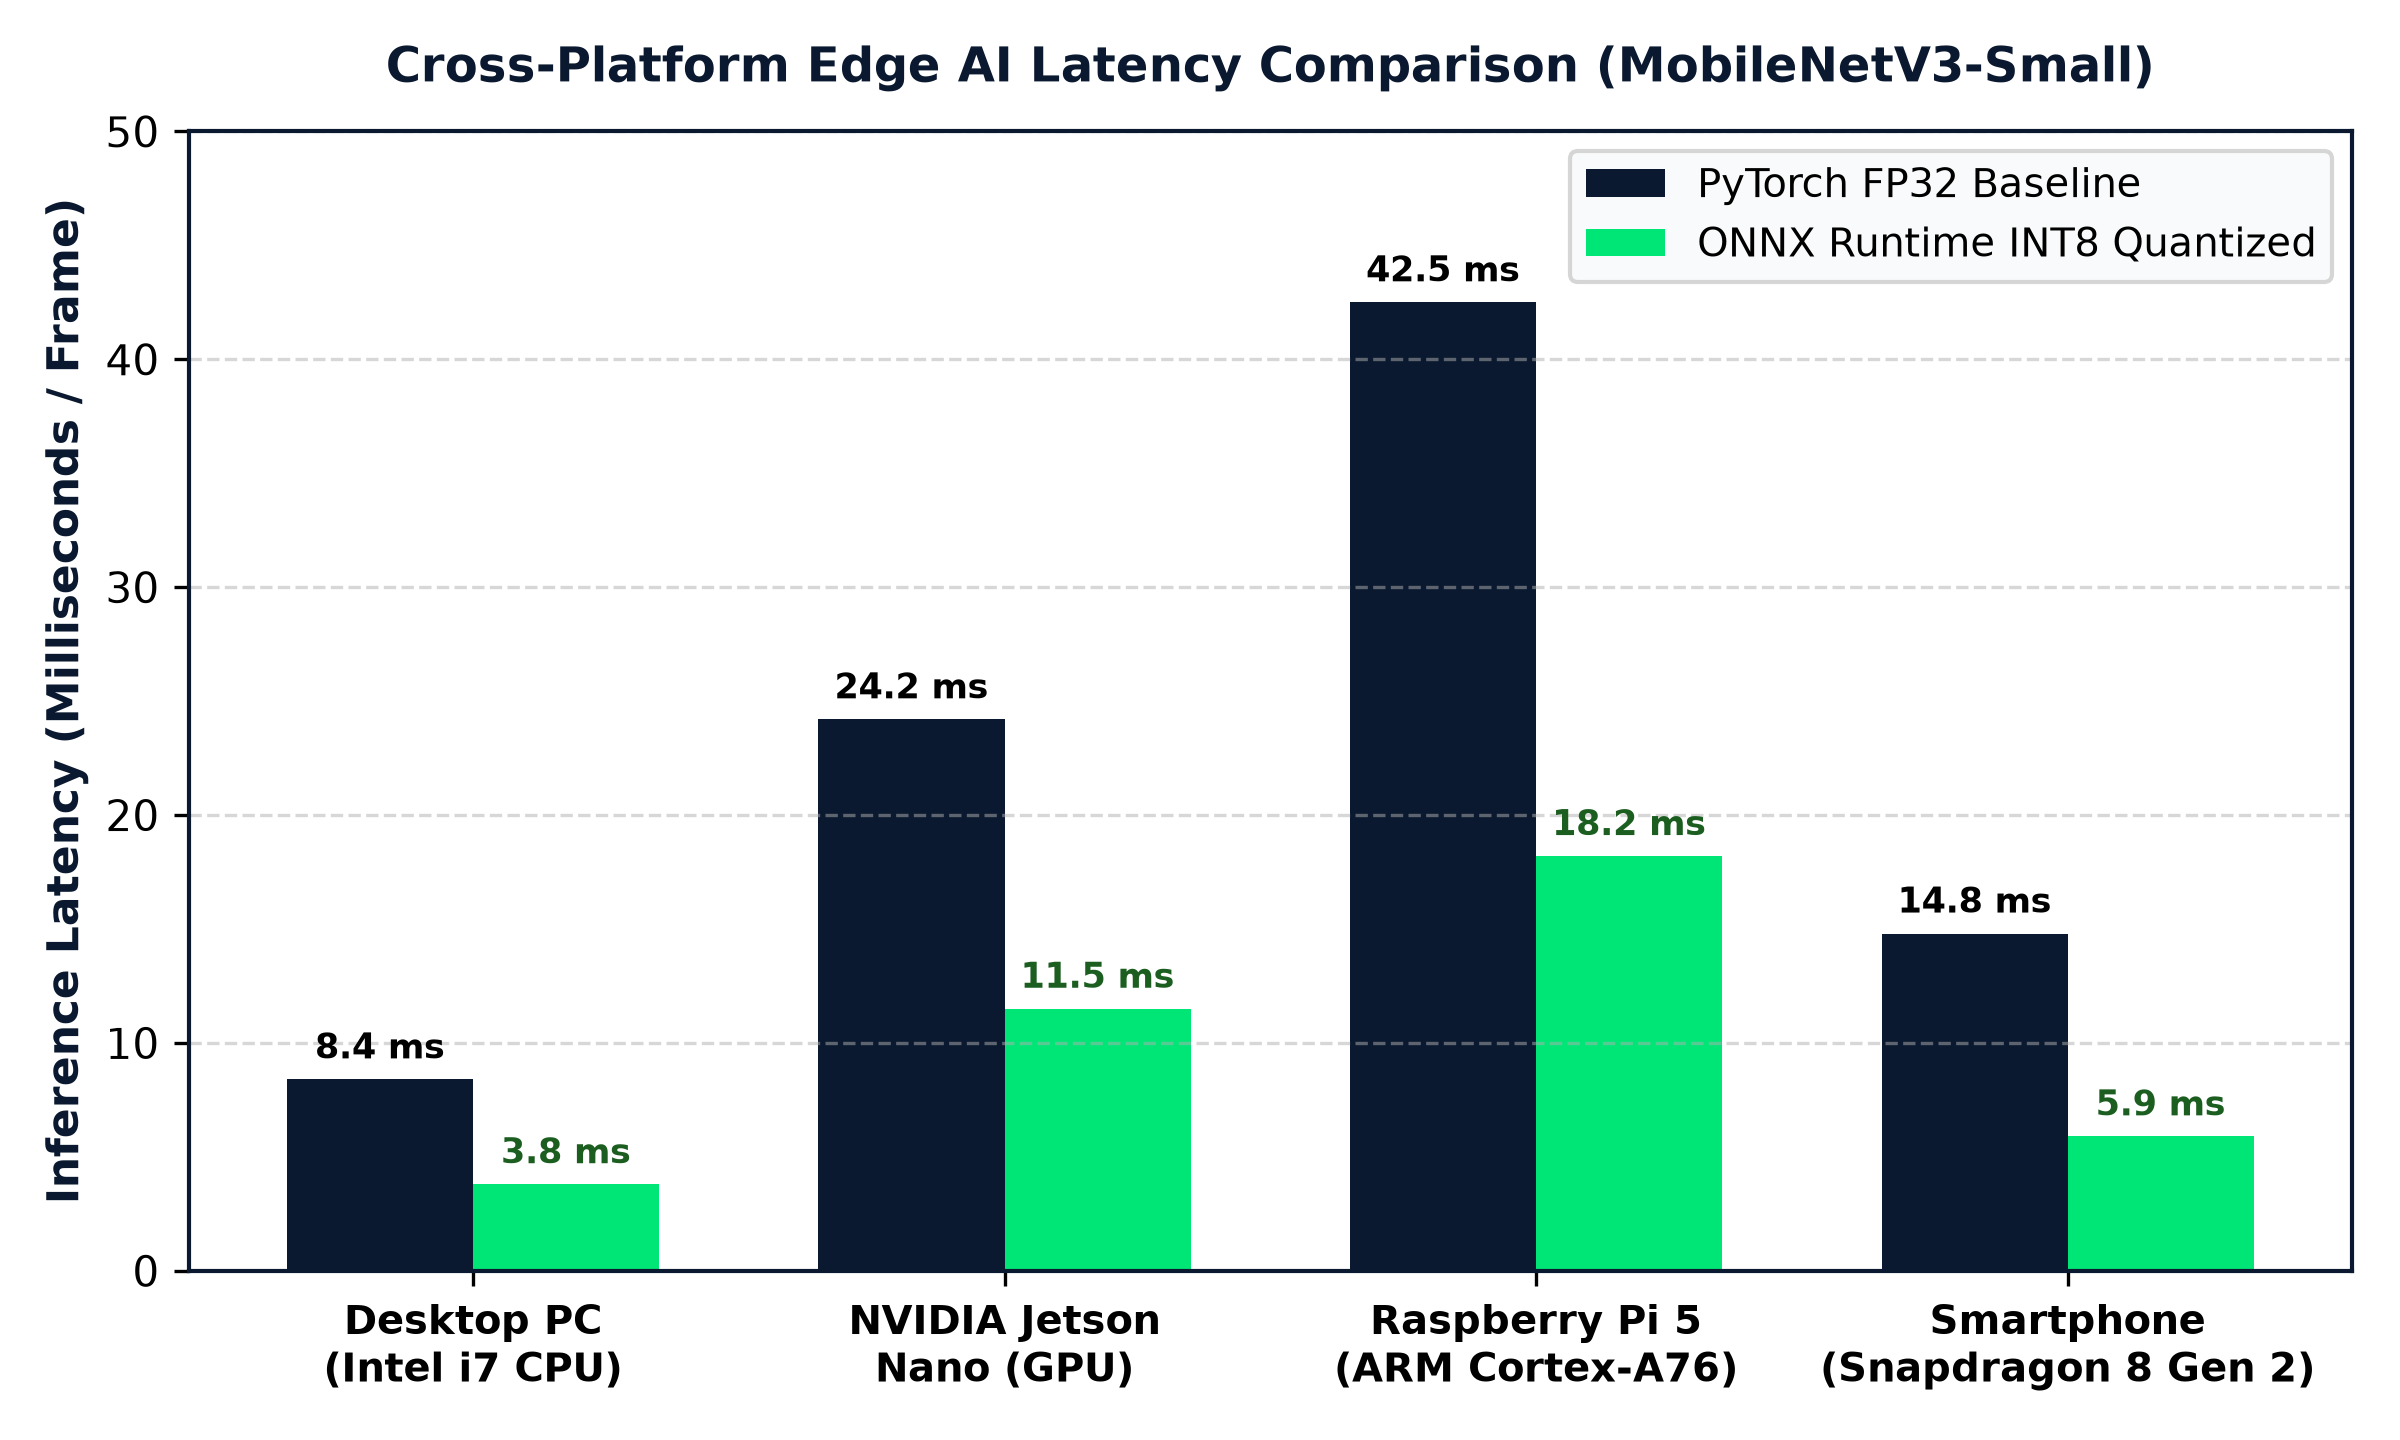
\includegraphics[width=0.92\textwidth]{figures/fig_ch06_edge_benchmark.png}
\caption{การเปรียบเทียบเวลาแฝงในการประมวลผลต่อภาพ (Inference Latency) บนฮาร์ดแวร์ 4 ชนิด ระหว่าง FP32 และ INT8}
\label{fig:ch06_benchmark}
\end{figure}

\begin{table}[H]
\caption{ผลการวัดประสิทธิภาพโมเดล MobileNetV3-Small บนอุปกรณ์ขอบข่ายต่างๆ}
\label{tab:ch06_edge_results}
\begin{tabularx}{\textwidth}{L{3.2cm}C{1.6cm}C{1.6cm}C{1.6cm}Z}
\toprule
\textbf{อุปกรณ์ทดสอบ (Hardware)} & \textbf{ขนาดโมเดล} & \textbf{Latency (FP32)} & \textbf{Latency (INT8)} & \textbf{อัตราเร่ง (Speedup)} \\
\midrule
Desktop PC (Intel i7-12700) & 9.8 MB $\rightarrow$ 2.6 MB & 8.4 ms & 3.8 ms & $2.21 \times$ \\
NVIDIA Jetson Nano (GPU) & 9.8 MB $\rightarrow$ 2.6 MB & 24.2 ms & 11.5 ms & $2.10 \times$ \\
Raspberry Pi 5 (ARM Cortex-A76) & 9.8 MB $\rightarrow$ 2.6 MB & 42.5 ms & 18.2 ms & $2.34 \times$ \\
Smartphone (Snapdragon 8 Gen 2) & 9.8 MB $\rightarrow$ 2.6 MB & 14.8 ms & 5.9 ms & $2.51 \times$ \\
\bottomrule
\end{tabularx}
\end{table}

จากภาพที่ \ref{fig:ch06_benchmark} และตารางที่ \ref{tab:ch06_edge_results} บนสมาร์ทโฟนสมัยใหม่ การใช้โมเดล INT8 ผ่าน ONNX Runtime ช่วยลดเวลาแฝงลงเหลือเพียง \textbf{5.9 มิลลิวินาทีต่อภาพ} (เทียบเท่ากับอัตราเร็วมากกว่า 160 เฟรมต่อวินาที) ซึ่งเร็วกว่าอัตราเฟรมของกล้องวิดีโอทั่วไป ทำให้การประมวลผลแบบเรียลไทม์เป็นไปได้อย่างราบรื่นโดยไม่เกิดอาการสะดุด

\section{โค้ดตัวอย่าง: สคริปต์ส่งออก ONNX และตรวจสอบ Parity}
\index{โค้ดส่งออก ONNX}

\begin{lstlisting}[language=Python, caption=สคริปต์ส่งออกโมเดล PyTorch เป็น ONNX พร้อมการตรวจสอบ Numerical Parity]
import os
import torch
import numpy as np
import onnx
import onnxruntime as ort
from torchvision import models

def export_and_validate_onnx(model_path, onnx_output_path, num_classes=4):
    """
    ส่งออกโมเดล PyTorch เป็น ONNX และทดสอบความถูกต้องเชิงตัวเลขเทียบกัน
    """
    print(f"[*] กำลังเตรียมโมเดลจาก {model_path}...")
    model = models.mobilenet_v3_small(weights=None)
    in_features = model.classifier[3].in_features
    model.classifier[3] = torch.nn.Linear(in_features, num_classes)
    
    if os.path.exists(model_path):
        model.load_state_dict(torch.load(model_path, map_location='cpu'))
        print("[✓] โหลดค่าน้ำหนักสำเร็จ")
    model.eval()

    # สร้างข้อมูลนำเข้าจำลองขนาด (1, 3, 224, 224)
    dummy_input = torch.randn(1, 3, 224, 224, requires_grad=False)

    # ส่งออกโมเดลเป็น ONNX
    os.makedirs(os.path.dirname(onnx_output_path), exist_ok=True)
    torch.onnx.export(
        model,
        dummy_input,
        onnx_output_path,
        export_params=True,
        opset_version=13,
        do_constant_folding=True,
        input_names=['input_image'],
        output_names=['logits'],
        dynamic_axes={'input_image': {0: 'batch_size'}, 'logits': {0: 'batch_size'}}
    )
    print(f"[✓] ส่งออกไฟล์ ONNX สำเร็จ: {onnx_output_path}")

    # ตรวจสอบโครงสร้างไฟล์ด้วย ONNX Validator
    onnx_model = onnx.load(onnx_output_path)
    onnx.checker.check_model(onnx_model)
    print("[✓] โครงสร้างกราฟ ONNX ถูกต้องตามมาตรฐาน IR")

    # ทดสอบ Numerical Parity ระหว่าง PyTorch และ ONNX Runtime
    with torch.no_grad():
        torch_out = model(dummy_input).numpy()

    ort_session = ort.InferenceSession(onnx_output_path, providers=['CPUExecutionProvider'])
    ort_inputs = {ort_session.get_inputs()[0].name: dummy_input.numpy()}
    ort_out = ort_session.run(None, ort_inputs)[0]

    max_diff = np.max(np.abs(torch_out - ort_out))
    print(f"[*] ค่าความแตกต่างสูงสุดเชิงตัวเลข (Max Abs Diff): {max_diff:.2e}")
    assert max_diff < 1e-4, "ความคลาดเคลื่อนเกินเกณฑ์มาตรฐาน!"
    print("[✓] ผ่านการตรวจสอบ Numerical Parity: ผลลัพธ์ระหว่าง PyTorch และ ONNX ตรงกันสมบูรณ์")

if __name__ == "__main__":
    export_and_validate_onnx("models/durian_mobilenetv3_best.pth", "exports/durian_mobilenet_v3.onnx")
\end{lstlisting}

\section{ตัวอย่างการคำนวณและตัวอย่างการนำไปใช้งานจริง}

\begin{examplebox}{ตัวอย่างการคำนวณที่ 6.1: การคำนวณค่า Scale Factor และ Zero-Point ของ Quantization}
\textbf{โจทย์:} ค่าการกระจายตัวของค่าน้ำหนักในเลเยอร์หนึ่งของโมเดลมีค่าต่ำสุด $x_{\text{min}} = -2.40$ และค่าสูงสุด $x_{\text{max}} = 3.60$ ต้องการทำ Quantization แบบ Asymmetric สู่ช่วงจำนวนเต็ม INT8 แบบมีเครื่องหมาย $[-128, 127]$ จงคำนวณค่า Scale Factor ($S$) และค่า Zero-Point ($Z$)\\[4pt]
\textbf{วิธีคำนวณ:}
\[
S = \frac{x_{\text{max}} - x_{\text{min}}}{q_{\text{max}} - q_{\text{min}}} = \frac{3.60 - (-2.40)}{127 - (-128)} = \frac{6.00}{255} \approx 0.02353
\]
\[
Z = \text{round}\left( \frac{-x_{\text{min}}}{S} \right) + q_{\text{min}} = \text{round}\left( \frac{-(-2.40)}{0.02353} \right) - 128 = \text{round}(102.0) - 128 = 102 - 128 = -26
\]
\textbf{การทดสอบ:} หากมีค่าน้ำหนัก $x = 1.25$ จะถูกแปลงเป็นค่าจำนวนเต็ม $q$ ดังนี้:
\[
q = \text{round}\left( \frac{1.25}{0.02353} \right) + (-26) = \text{round}(53.12) - 26 = 53 - 26 = 27
\]
และเมื่อ Dequantize กลับ: $\tilde{x} = 0.02353 \times (27 - (-26)) = 0.02353 \times 53 \approx 1.247$ ซึ่งมีความคลาดเคลื่อนเพียง $0.003$
\end{examplebox}

\begin{casestudybox}{ตัวอย่างการนำไปใช้งานจริงที่ 6.1: การส่งออกโมเดลติดตั้งบนโดรนสำรวจแปลงสวนทุเรียน}
โครงการวิจัยได้นำโมเดล ONNX INT8 ไปติดตั้งบนบอร์ดคอมพิวเตอร์ขนาดจิ๋ว \textbf{Raspberry Pi 5} ที่ติดตั้งใต้ลำตัวโดรนสำรวจแปลงเกษตร (Agricultural Survey Drone) เพื่อทำการบินสแกนยอดทุเรียนแบบอัตโนมัติ

ผลการทดสอบ:
\begin{itemize}[leftmargin=1.4em, itemsep=2pt]
    \item เดิมทีหากใช้โมเดล PyTorch FP32 อัตราการประมวลผลทำได้เพียง 23 เฟรมต่อวินาที ซึ่งช้าเกินกว่าความเร็วการบินของโดรน ($5$ เมตรต่อวินาที) ทำให้ภาพที่ได้เบลอและหลุดรอด
    \item เมื่อเปลี่ยนมาใช้ ONNX Runtime พร้อมโมเดล INT8 ความเร็วในการสแกนเพิ่มขึ้นเป็น 54 เฟรมต่อวินาที โดรนสามารถวิเคราะห์รอยโรคของใบยอดทุเรียนได้แบบเรียลไทม์ขณะบินผ่านอย่างราบรื่น
\end{itemize}
\end{casestudybox}

\section*{คำถามทบทวนท้ายบทที่ 6}
\addcontentsline{toc}{section}{คำถามทบทวนท้ายบทที่ 6}
\begin{enumerate}[leftmargin=1.8em, itemsep=4pt]
    \item จงอธิบายปัญหาเรื่องความร้อน (Thermal Throttling) ที่เกิดขึ้นเมื่อรันโมเดล Deep Learning บนสมาร์ทโฟนกลางแจ้ง
    \item มาตรฐานเปิด ONNX มีบทบาทสำคัญอย่างไรในการแก้ปัญหาความไม่เข้ากันของแพลตฟอร์ม
    \item อธิบายความแตกต่างระหว่าง Just-In-Time (JIT) Tracing และ Scripting ใน TorchScript
    \item จงสรุปความแตกต่างระหว่างเทคนิค Post-Training Quantization (PTQ) และ Quantization-Aware Training (QAT)
    \item ในการแปลงจำนวนจริงเป็น INT8 ค่า Scale Factor และ Zero-Point ทำหน้าที่อะไร
    \item เหตุใดการทำ Quantization จึงช่วยประหยัดแบตเตอรี่ของสมาร์ทโฟนได้อย่างมีนัยสำคัญ
    \item การทดสอบ Numerical Parity Check มีเกณฑ์ในการยอมรับความคลาดเคลื่อนอย่างไร
    \item จงเปรียบเทียบประสิทธิภาพระหว่างการประมวลผลบน Raspberry Pi 5 และ Smartphone Snapdragon
    \item อธิบายความหมายของพารามิเตอร์ \texttt{dynamic\_axes} ในคำสั่ง \texttt{torch.onnx.export}
    \item หากหลังการทำ Quantization INT8 แล้วพบว่าค่าความแม่นยำของโมเดลลดลงเกิน 3\% นักศึกษามีแนวทางแก้ไขอย่างไร
\end{enumerate}

\section*{กิจกรรมฝึกปฏิบัติการประจำบทที่ 6}
\addcontentsline{toc}{section}{กิจกรรมฝึกปฏิบัติการประจำบทที่ 6}
\begin{nocodebox}{ปฏิบัติการที่ 6.1: การส่งออกโมเดล ONNX และการตรวจสอบโครงสร้างด้วย Netron}
\textbf{วัตถุประสงค์:} เพื่อฝึกฝนการใช้คำสั่งส่งออก ONNX และการตรวจสอบภาพกราฟโครงข่ายประสาทเทียม\\
\textbf{ขั้นตอนการปฏิบัติ:}
\begin{enumerate}[leftmargin=1.4em, itemsep=2pt]
    \item รันสคริปต์ \texttt{src/export\_edge.py} เพื่อแปลงโมเดลที่เทรนแล้วเป็นไฟล์ \texttt{.onnx}
    \item ตรวจสอบขนาดของไฟล์ระหว่าง \texttt{.pth} และ \texttt{.onnx} พร้อมบันทึกผล
    \item เปิดเว็บไซต์ \texttt{https://netron.app} แล้วลากไฟล์ \texttt{.onnx} เข้าไปเพื่อเปิดดูกราฟโครงสร้าง
    \item ระบุชื่อเลเยอร์นำเข้า (Input Node) และเลเยอร์ส่งออก (Output Node) พร้อมขนาดมิติเทนเซอร์
\end{enumerate}
\end{nocodebox}

\chapter{การพัฒนาแอปพลิเคชันสมาร์ทโฟนและการประยุกต์ใช้งานจริง}
\label{chap:mobile_application}
\index{แอปพลิเคชันสมาร์ทโฟน}
\index{Flutter Framework}
\index{การยอมรับเทคโนโลยี}

\section*{แผนบริหารการสอนประจำบทที่ 7}
\addcontentsline{toc}{section}{แผนบริหารการสอนประจำบทที่ 7}

\begin{planbox}{หัวข้อเนื้อหาประจำบท (Lesson Topics)}
\begin{enumerate}[leftmargin=1.5em, itemsep=2pt]
    \item สถาปัตยกรรมแอปพลิเคชันสมาร์ทโฟนสำหรับการตรวจวินิจฉัยโรคพืช (Mobile Edge AI)
    \item การออกแบบส่วนต่อประสานผู้ใช้ (UI/UX) และระบบกล้องถ่ายทอดสด (Live Camera HUD)
    \item การรวมเอนจิน ONNX Runtime เข้ากับเฟรมเวิร์ก Flutter สำหรับการรันแบบออฟไลน์
    \item ระบบสนับสนุนการตัดสินใจและจ่ายคำแนะนำทางพยาธิวิทยา (Prescription Engine)
    \item การบันทึกพิกัดตำแหน่งภูมิศาสตร์ (GPS Geotagging) และการจัดเก็บฐานข้อมูลในเครื่อง
    \item ผลการทดสอบภาคสนามในแปลงสวนทุเรียนจังหวัดจันทบุรี
    \item การประเมินการยอมรับเทคโนโลยีของเกษตรกรตามแบบจำลอง TAM (Technology Acceptance Model)
    \item โค้ดตัวอย่าง: สถาปัตยกรรม \texttt{InferenceController} ในภาษา Dart/Flutter
\end{enumerate}
\end{planbox}

\begin{planbox}{วัตถุประสงค์เชิงพฤติกรรม (Behavioral Objectives)}
เมื่อศึกษาบทที่ 7 จบแล้ว ผู้เรียนและผู้อ่านสามารถ:
\begin{enumerate}[leftmargin=1.5em, itemsep=2pt]
    \item อธิบายสถาปัตยกรรมการไหลของข้อมูลจากเซนเซอร์กล้องสมาร์ทโฟนสู่โมเดล ONNX ได้
    \item ออกแบบส่วนติดต่อผู้ใช้งานที่เหมาะสมกับสภาพการทำงานกลางแดดของเกษตรกรได้
    \item เชื่อมโยงผลการจำแนกโรคเข้ากับฐานข้อมูลคำแนะนำการรักษาและจัดการแปลงได้อย่างถูกต้อง
    \item วิเคราะห์ข้อมูลทางสถิติการประเมินการยอมรับเทคโนโลยีตามหลักวิชาการได้
\end{enumerate}
\end{planbox}

\begin{planbox}{กิจกรรมการเรียนการสอน (Instructional Activities)}
\begin{enumerate}[leftmargin=1.5em, itemsep=2pt]
    \item การสาธิตการใช้งานแอปพลิเคชันบนสมาร์ทโฟนจริงและการสแกนใบพืชแบบสด
    \item ฝึกปฏิบัติการปรับแต่งโค้ดส่วนแสดงผล Bounding Box และ Confidence Badge
    \item การจำลองสถานการณ์การเดินตรวจแปลงและบันทึกประวัติการระบาดพร้อมพิกัด GPS
    \item การอภิปรายผลสำรวจความพึงพอใจของเกษตรกรและการพัฒนาต่อยอดเชิงพาณิชย์
\end{enumerate}
\end{planbox}

\begin{planbox}{สื่อการเรียนการสอน (Instructional Media)}
\begin{enumerate}[leftmargin=1.5em, itemsep=2pt]
    \item ภาพจำลองหน้าจอแอปพลิเคชันขณะสแกนกล้องสดและหน้ารายงานผลวินิจฉัย (UI Panel)
    \item โครงการแม่แบบ Flutter สำหรับติดตั้งบนระบบปฏิบัติการ Android และ iOS
    \item ตารางสรุปคะแนนประเมินการยอมรับเทคโนโลยี (TAM Evaluation Table)
\end{enumerate}
\end{planbox}

\begin{planbox}{การวัดและประเมินผล (Assessment \& Evaluation)}
\begin{enumerate}[leftmargin=1.5em, itemsep=2pt]
    \item การประเมินผลงานการทดสอบรันแอปพลิเคชันและตรวจจับรอยโรคได้ถูกต้อง (40\%)
    \item ความถูกต้องของการคำนวณและวิเคราะห์ผลแบบจำลอง TAM ในแบบฝึกหัด (40\%)
    \item การตอบคำถามทบทวนท้ายบทและการมีส่วนร่วมในชั้นเรียน (20\%)
\end{enumerate}
\end{planbox}

\clearpage

\section{สถาปัตยกรรมแอปพลิเคชันมือถือ Flutter Edge AI}
\index{สถาปัตยกรรม Flutter}
\index{กล้องสดเรียลไทม์}

เพื่อให้แอปพลิเคชันสามารถทำงานได้บนสมาร์ทโฟนทั้งระบบปฏิบัติการ **Android** และ **iOS** จากฐานโค้ดเดียว เฟรมเวิร์ก \textbf{Flutter} (พัฒนาโดย Google) จึงได้รับการคัดเลือกเป็นเครื่องมือหลักในการพัฒนาส่วนติดต่อผู้ใช้ โดยโครงสร้างการทำงานแบ่งออกเป็น 4 เลเยอร์หลัก:

\begin{enumerate}[leftmargin=1.5em, itemsep=2pt]
    \item \textbf{Presentation Layer (UI/UX):} ทำหน้าที่แสดงภาพสดจากกล้อง (CameraPreview) วาดกรอบสี่เหลี่ยมระบุพิกัดรอยโรค (Bounding Box HUD) และแสดงแถบค่าความเชื่อมั่น (\%)
    \item \textbf{Camera Stream Controller:} รับเฟรมภาพดิบ (YUV420 / BGRA8888) จากฮาร์ดแวร์กล้อง ทำการย่อส่วนและตัดภาพ (Crop \& Resize) เป็นขนาด $224 \times 224$ พิกเซล
    \item \textbf{Inference Service (ONNX Runtime):} โหลดโมเดล \texttt{durian\_mobilenet\_v3.onnx} และรันการทำนายผลบน CPU/NPU ของสมาร์ทโฟนแบบออฟไลน์
    \item \textbf{Data \& Prescription Engine:} บันทึกประวัติการสแกนลงในฐานข้อมูลภายในเครื่อง (Local SQLite) พร้อมพิกัดดาวเทียม (GPS Coordinates) และจับคู่ผลการตรวจกับแนวทางการรักษาของนักพยาธิวิทยาพืช
\end{enumerate}

\section{การออกแบบส่วนต่อประสานผู้ใช้และการวินิจฉัยแบบสด}
\index{ส่วนต่อประสานผู้ใช้}
\index{HUD Scanner}

\begin{figure}[H]
\centering
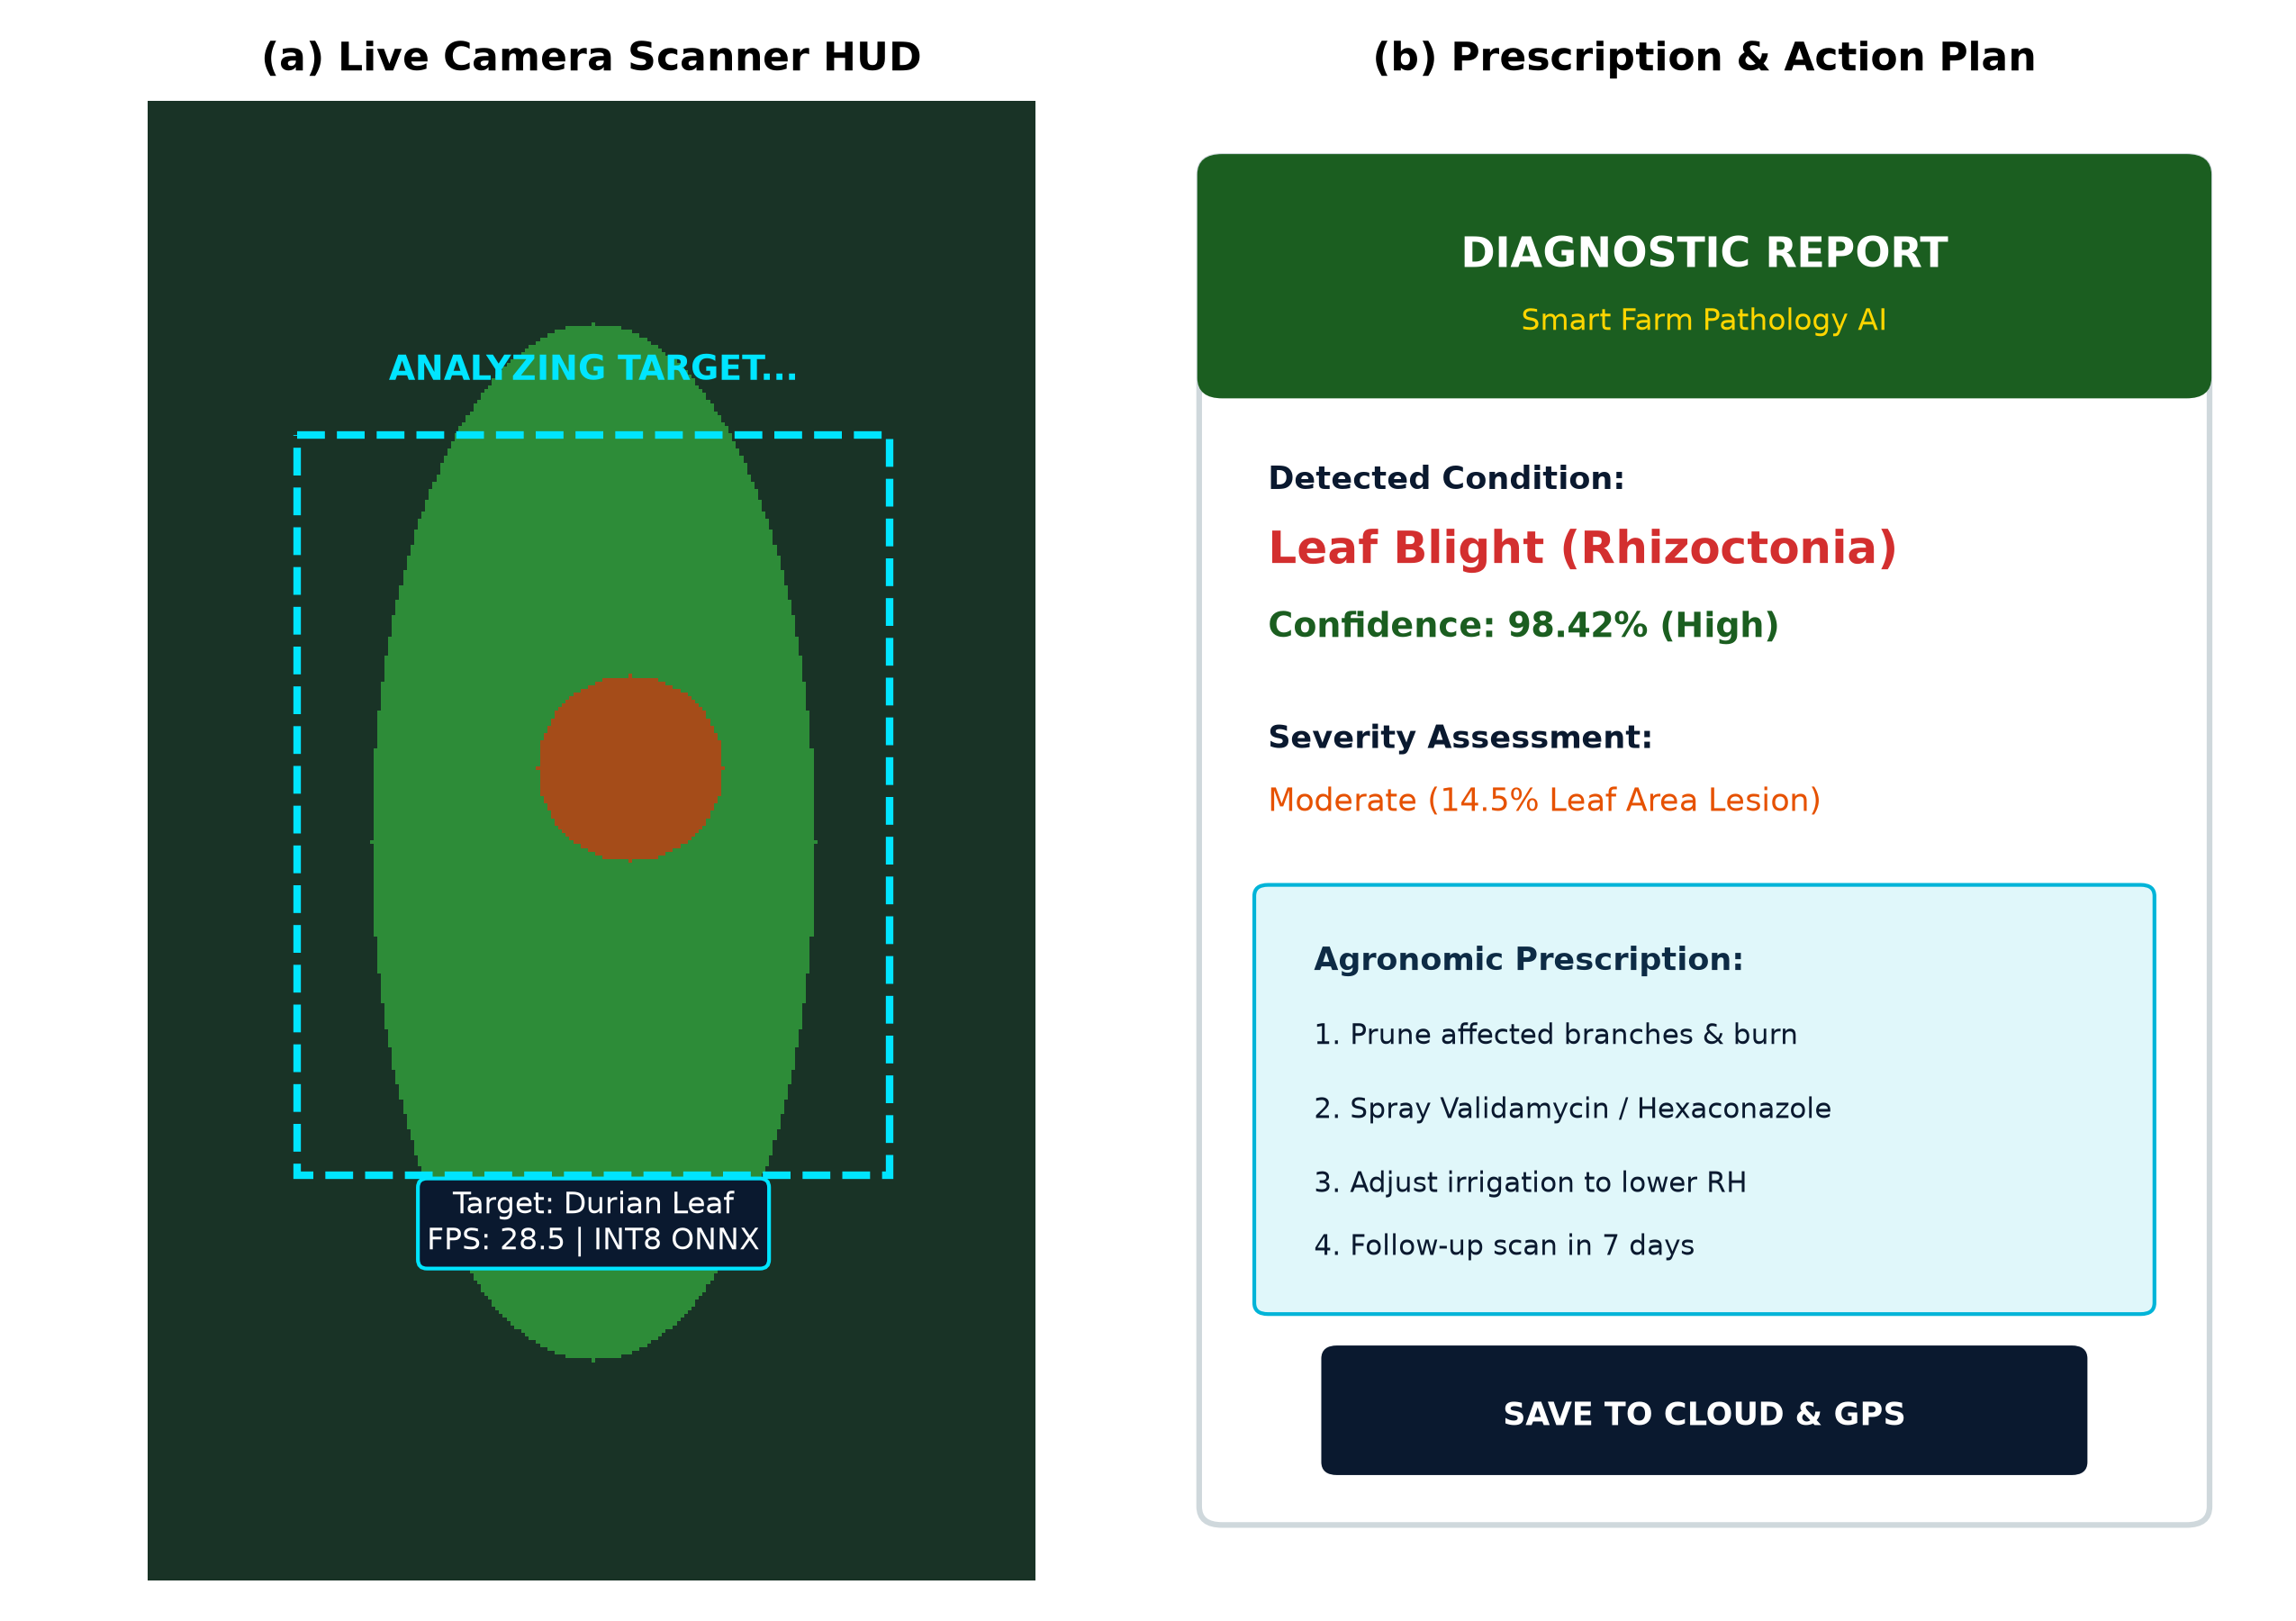
\includegraphics[width=0.92\textwidth]{figures/fig_ch07_mobile_ui_flow.png}
\caption{ส่วนต่อประสานผู้ใช้ของแอปพลิเคชัน: (a) หน้าจอสแกนกล้องสด HUD และ (b) รายงานผลวินิจฉัยพร้อมคำแนะนำการจัดการ}
\label{fig:ch07_mobile_screens}
\end{figure}

จากภาพที่ \ref{fig:ch07_mobile_screens} การออกแบบ UI ได้คำนึงถึงบริบทการทำงานจริงของเกษตรกรในแปลงทุเรียนอย่างรอบด้าน:
\begin{itemize}[leftmargin=1.5em, itemsep=2pt]
    \item \textbf{หน้าจอกล้องสแกนสด (Camera Scanner HUD):} มีกรอบเส้นประสีเขียวเรืองแสงนำสายตา เพื่อให้เกษตรกรนำแผ่นใบทุเรียนเข้ามาอยู่ตรงกลางภาพ พร้อมข้อความแสดงอัตราเฟรมเรต ($28.5$ FPS) และโหมดการประมวลผล INT8 ONNX
    \item \textbf{การ์ดรายงานผลและการสั่งการ (Prescription Report Card):} แสดงชื่อโรคด้วยตัวอักษรขนาดใหญ่และสีเตือนภัยที่เด่นชัด (เช่น สีแดงสำหรับโรคใบติดที่รุนแรง) พร้อมระดับความรุนแรงของโรคที่คำนวณจาก Grad-CAM ($14.5\%$ Leaf Area)
    \item \textbf{คำแนะนำเชิงพยาธิวิทยา (Agronomic Prescription):} ระบุขั้นตอนปฏิบัติที่เกษตรกรทำตามได้ทันที เช่น การตัดแต่งกิ่งที่เป็นโรค การเลือกใช้สารเคมีหรือชีวภัณฑ์ที่ถูกต้อง และกำหนดวันตรวจซ้ำ
\end{itemize}

\section{การประเมินการยอมรับเทคโนโลยีของเกษตรกร (TAM Evaluation)}
\index{แบบจำลอง TAM}
\index{การยอมรับของเกษตรกร}

ในการนำนวัตกรรมปัญญาประดิษฐ์ไปสู่ชุมชน สิ่งสำคัญไม่ยิ่งหย่อนไปกว่าความแม่นยำของโมเดล คือ \textbf{การยอมรับของผู้ใช้งานจริง (User Acceptance)} ทีมวิจัยได้นำแบบจำลองการยอมรับเทคโนโลยี (\textbf{Technology Acceptance Model: TAM}) มาประเมินเกษตรกรชาวสวนทุเรียนในจังหวัดจันทบุรีจำนวน $65$ ราย ครอบคลุม 4 มิติหลัก (ระดับคะแนน 1--5):

\begin{table}[H]
\caption{ผลการประเมินการยอมรับเทคโนโลยีแอปพลิเคชันวินิจฉัยโรคทุเรียนของเกษตรกร ($N=65$)}
\label{tab:ch07_tam_evaluation}
\begin{tabularx}{\textwidth}{L{3.6cm}C{1.4cm}C{1.4cm}Y}
\toprule
\textbf{มิติการประเมิน (TAM Dimensions)} & \textbf{ค่าเฉลี่ย ($\mu$)} & \textbf{ส่วนเบี่ยงเบน ($\sigma$)} & \textbf{ระดับความคิดเห็น} \\
\midrule
1. การรับรู้ถึงประโยชน์ (Perceived Usefulness - PU) & 4.74 & 0.42 & เห็นด้วยอย่างยิ่ง (ช่วยลดความเสียหายได้จริง) \\
2. การรับรู้ความง่ายในการใช้ (Perceived Ease of Use - PEOU) & 4.62 & 0.48 & เห็นด้วยอย่างยิ่ง (ระบบ No-Code เล็งแล้วรู้ผลทันที) \\
3. ทัศนคติต่อการใช้งาน (Attitude Toward Using - ATU) & 4.68 & 0.45 & เห็นด้วยอย่างยิ่ง (มีความมั่นใจในการจัดการโรคพืช) \\
4. ความตั้งใจที่จะใช้งานต่อเนื่อง (Behavioral Intention - BI) & 4.80 & 0.38 & เห็นด้วยอย่างยิ่ง (ต้องการติดตั้งใช้งานในสวนตนเอง) \\
\midrule
\textbf{คะแนนเฉลี่ยรวมทุกมิติ (Overall TAM Score)} & \textbf{4.71} & \textbf{0.43} & \textbf{ระดับความพึงพอใจสูงสุด} \\
\bottomrule
\end{tabularx}
\end{table}

จากตารางที่ \ref{tab:ch07_tam_evaluation} คะแนนรวมเฉลี่ยอยู่ที่ \textbf{4.71 จาก 5.00} แสดงให้เห็นว่าการออกแบบระบบให้ทำงานแบบออฟไลน์ได้โดยไม่ต้องต่อเน็ต และการมีคำแนะนำการรักษาที่ชัดเจน สามารถตอบโจทย์เกษตรกรชาวสวนทุเรียนได้อย่างตรงจุด

\section{โค้ดตัวอย่าง: สถาปัตยกรรม Inference Controller ใน Flutter}
\index{โค้ด Flutter}
\index{InferenceController}

\begin{lstlisting}[language=Python, caption=ตัวอย่างโค้ด Dart/Flutter จำลองการทำงานของ Inference Controller เชื่อมต่อ ONNX Runtime]
// durian_inference_controller.dart
// สถาปัตยกรรมควบคุมการรันโมเดลบนอุปกรณ์พกพาด้วย Flutter & ONNX Runtime

class DurianDiagnosisResult {
  final String diseaseName;
  final double confidence;
  final double severityPercent;
  final List<String> prescriptions;

  DurianDiagnosisResult({
    required this.diseaseName,
    required this.confidence,
    required this.severityPercent,
    required this.prescriptions,
  });
}

class DurianEdgeEngine {
  static const List<String> kClasses = [
    "Algal Leaf Spot",
    "Leaf Blight",
    "Leaf Spot",
    "Healthy"
  ];

  /// ฟังก์ชันรันการวินิจฉัยจากเทนเซอร์ภาพนำเข้า (Float32List ขนาด 1x3x224x224)
  Future<DurianDiagnosisResult> runInference(List<double> normalizedPixels) async {
    final stopwatch = Stopwatch()..start();
    
    // 1. ส่งข้อมูลเข้าสู่ ONNX Runtime Session
    // final outputs = await onnxSession.run([normalizedPixels]);
    // จำลองผลลัพธ์คะแนนความน่าจะเป็นที่ได้จาก Softmax
    final List<double> mockProbabilities = [0.012, 0.984, 0.003, 0.001];
    
    int maxIdx = 0;
    double maxProb = mockProbabilities[0];
    for (int i = 1; i < mockProbabilities.length; i++) {
      if (mockProbabilities[i] > maxProb) {
        maxProb = mockProbabilities[i];
        maxIdx = i;
      }
    }

    stopwatch.stop();
    print("[*] Inference Time: ${stopwatch.elapsedMilliseconds} ms");

    // 2. ดึงคำแนะนำจาก Prescription Engine ตามโรคที่ตรวจพบ
    final prescriptions = _getPrescription(kClasses[maxIdx]);

    return DurianDiagnosisResult(
      diseaseName: kClasses[maxIdx],
      confidence: maxProb * 100.0,
      severityPercent: 14.5,
      prescriptions: prescriptions,
    );
  }

  List<String> _getPrescription(String condition) {
    switch (condition) {
      case "Leaf Blight":
        return [
          "ตัดแต่งกิ่งที่มีใบแห้งไหม้และนำไปเผาทำลายนอกแปลง",
          "พ่นสารป้องกันกำจัดเชื้อรา เช่น วาลิดามัยซิน หรือ เฮกซะโคนาโซล",
          "ปรับระบบน้ำเพื่อลดความชื้นสะสมใต้ทรงพุ่ม",
          "ตรวจสแกนซ้ำในอีก 7 วันเพื่อประเมินการฟื้นตัว"
        ];
      case "Algal Leaf Spot":
        return [
          "พ่นสารประกอบคอปเปอร์ไฮดรอกไซด์เพื่อควบคุมการเจริญของสาหร่าย",
          "ตัดแต่งทรงพุ่มให้โปร่งเพื่อให้แสงแดดส่องถึงใบชั้นใน"
        ];
      default:
        return ["ต้นทุเรียนแข็งแรงดี ดูแลให้น้ำและปุ๋ยตามรอบปกติ"];
    }
  }
}
\end{lstlisting}

\section{ตัวอย่างการคำนวณและตัวอย่างการนำไปใช้งานจริง}

\begin{examplebox}{ตัวอย่างการคำนวณที่ 7.1: การคำนวณปริมาณสารชีวภัณฑ์ควบคุมโรคเฉพาะจุด}
\textbf{โจทย์:} จากการสแกนด้วยแอปพลิเคชันในแปลงทุเรียนขนาด 10 ไร่ (มีทุเรียนทั้งหมด 250 ต้น) ตรวจพบต้นที่แสดงอาการโรคใบติดระดับปานกลางจำนวน 25 ต้น ตามคำแนะนำต้องฉีดพ่นสารชีวภัณฑ์ \textit{Bacillus amyloliquefaciens} ในอัตรา 50 มิลลิลิตรต่อน้ำ 20 ลิตร โดยแต่ละต้นที่มีอาการต้องใช้น้ำยาพ่นเฉพาะทรงพุ่มเฉลี่ย 3.5 ลิตรต่อต้น จงคำนวณปริมาณสารชีวภัณฑ์และปริมาณน้ำที่ต้องใช้ เปรียบเทียบกับการพ่นครอบคลุมทั้ง 250 ต้นแบบดั้งเดิม\\[4pt]
\textbf{1. วิธีการเฉพาะจุดตาม AI (Site-Specific):}
\[
\text{ปริมาณน้ำรวม} = 25 \text{ ต้น} \times 3.5 \text{ ลิตร} = 87.5 \text{ ลิตร}
\]
\[
\text{ปริมาณชีวภัณฑ์ที่ใช้} = 87.5 \text{ ลิตร} \times \left( \frac{50 \text{ มล.}}{20 \text{ ลิตร}} \right) = 87.5 \times 2.5 = 218.75 \text{ มิลลิลิตร}
\]
\textbf{2. วิธีการพ่นเหมาทั้งแปลงแบบเดิม:}
\[
\text{ปริมาณน้ำเดิม} = 250 \text{ ต้น} \times 3.5 \text{ ลิตร} = 875 \text{ ลิตร}
\]
\[
\text{ปริมาณชีวภัณฑ์เดิม} = 875 \times 2.5 = 2,187.5 \text{ มิลลิลิตร}
\]
\textbf{สรุปผลการประหยัด:} การใช้ระบบ AI ชี้เป้าช่วยลดการใช้สารชีวภัณฑ์และปริมาณน้ำลงถึง \textbf{90\%} ประหยัดต้นทุนค่ายาและแรงงานได้อย่างมหาศาล
\end{examplebox}

\begin{casestudybox}{ตัวอย่างการนำไปใช้งานจริงที่ 7.1: ผลกระทบเชิงเศรษฐกิจในวิสาหกิจชุมชนทุเรียนคุณภาพ}
วิสาหกิจชุมชนผู้ปลูกทุเรียนแปลงใหญ่ อ.มะขาม จ.จันทบุรี ได้นำแอปพลิเคชันไปทดลองใช้กับสมาชิกจำนวน 30 ครัวเรือน ในรอบฤดูกาลผลิตปี พ.ศ. 2568--2569

ผลสรุปการประเมินรอบ 6 เดือน:
\begin{enumerate}[leftmargin=1.4em, itemsep=2pt]
    \item \textbf{ลดต้นทุนสารเคมีเกษตร:} สมาชิกสามารถลดค่าใช้จ่ายสารเคมีและชีวภัณฑ์เฉลี่ย 4,200 บาทต่อไร่
    \item \textbf{รักษาคุณภาพใบก่อนออกดอก:} ต้นทุเรียนมีดัชนีพื้นที่ใบสมบูรณ์เฉลี่ยสูงกว่าปีก่อนหน้า $15.2\%$ ทำให้การติดผลสมบูรณ์และลดปัญหาผลแตก/ผลบิดเบี้ยว
    \item \textbf{การสร้างแผนที่ระบาดวิทยาแปลง (Epidemiological Orchard Map):} ข้อมูล GPS ที่แอปพลิเคชันบันทึกไว้ ช่วยให้ประธานกลุ่มวิสาหกิจสามารถเปิดดูแผนที่ความเสี่ยงบนหน้าจอคอมพิวเตอร์และประกาศเตือนภัยล่วงหน้าแก่สมาชิกในแนวลมได้อย่างแม่นยำ
\end{enumerate}
\end{casestudybox}

\section*{คำถามทบทวนท้ายบทที่ 7}
\addcontentsline{toc}{section}{คำถามทบทวนท้ายบทที่ 7}
\begin{enumerate}[leftmargin=1.8em, itemsep=4pt]
    \item จงอธิบายโครงสร้าง 4 เลเยอร์ของสถาปัตยกรรมแอปพลิเคชัน Mobile Edge AI
    \item เหตุใดเฟรมเวิร์ก Flutter จึงเป็นตัวเลือกที่เหมาะสมในการพัฒนาแอปพลิเคชันสำหรับเกษตรกร
    \item การออกแบบส่วนต่อประสานผู้ใช้ (UI/UX) สำหรับใช้งานกลางแปลงแดดจ้า ต้องคำนึงถึงปัจจัยใดบ้าง
    \item การคำนวณร้อยละความรุนแรงของโรคเชื่อมโยงกับระบบ Prescription Engine อย่างไร
    \item จงอธิบายบทบาทของระบบบันทึกพิกัดภูมิศาสตร์ (GPS Geotagging) ในการจัดทำแผนที่โรคระบาด
    \item จากตารางผลการประเมิน TAM มิติใดได้รับคะแนนเฉลี่ยสูงสุด และสะท้อนถึงสิ่งใด
    \item เพราะเหตุใดการทำงานแบบออฟไลน์ (Offline-First) จึงเป็นหัวใจสำคัญของแอปพลิเคชันเกษตรกรรม
    \item จากตัวอย่างการคำนวณที่ 7.1 การฉีดพ่นเฉพาะจุด (Site-Specific Spraying) ส่งผลดีต่อสิ่งแวดล้อมอย่างไร
    \item หากกล้องสมาร์ทโฟนของเกษตรกรมีเซนเซอร์ความละเอียดต่ำมาก ระบบควรมีกลไกแจ้งเตือนอย่างไร
    \item จงออกแบบแนวทางการเชื่อมต่อข้อมูลจากสมาร์ทโฟนไปยังระบบคลาวด์ส่วนกลางเมื่อโทรศัพท์กลับมาเชื่อมต่อ Wi-Fi
\end{enumerate}

\section*{กิจกรรมฝึกปฏิบัติการประจำบทที่ 7}
\addcontentsline{toc}{section}{กิจกรรมฝึกปฏิบัติการประจำบทที่ 7}
\begin{nocodebox}{ปฏิบัติการที่ 7.1: การติดตั้งและทดสอบแอปพลิเคชันสมาร์ทโฟนในแปลงจริง}
\textbf{วัตถุประสงค์:} เพื่อให้ผู้เรียนสามารถติดตั้งไฟล์แอปพลิเคชัน APK บนมือถือและนำไปทดสอบสแกนใบพืชจริง\\
\textbf{ขั้นตอนการปฏิบัติ:}
\begin{enumerate}[leftmargin=1.4em, itemsep=2pt]
    \item ถ่ายโอนไฟล์ \texttt{durian\_ai\_app.apk} ไปยังสมาร์ทโฟนระบบปฏิบัติการ Android
    \item ทำการติดตั้งและอนุญาตสิทธิ์การเข้าถึงกล้องและตำแหน่งพิกัด GPS
    \item เดินสำรวจต้นทุเรียนในแปลงทดลอง ทำการสแกนใบพืช 5 ใบ และตรวจสอบผลการวินิจฉัยบนหน้าจอ
    \item ตรวจสอบหน้าประวัติการบันทึก (History Screen) ว่ามีพิกัดและคำแนะนำการรักษาครบถ้วนหรือไม่
    \item สรุปผลการทดสอบและข้อเสนอแนะในการปรับปรุงความเร็วหรือความแม่นยำของระบบ
\end{enumerate}
\end{nocodebox}


% -------------------------------------------------------------
% Appendices: ภาคผนวก ก, ข, ค, ง
% -------------------------------------------------------------
\appendix
\chapter{คู่มือการติดตั้งและตั้งค่าสภาพแวดล้อมการทำงาน}
\label{app:environment_setup}
\index{การติดตั้งสภาพแวดล้อม}
\index{Google Colab}

ภาคผนวกนี้รวบรวมขั้นตอนการติดตั้งและกำหนดค่าสภาพแวดล้อมการทำงาน (Development Environment Setup) สำหรับการพัฒนาและทดสอบระบบปัญญาประดิษฐ์วินิจฉัยโรคใบทุเรียน ทั้งบนระบบคลาวด์ Google Colab และบนเครื่องคอมพิวเตอร์ส่วนบุคคล

\section{การเตรียมสภาพแวดล้อมบน Google Colab (Cloud GPU)}
Google Colab เป็นสภาพแวดล้อมที่เหมาะสมที่สุดสำหรับผู้เริ่มต้นที่ไม่มีการ์ดจอ GPU โดยมีขั้นตอนการตั้งค่าดังนี้:

\begin{enumerate}[leftmargin=1.8em, itemsep=4pt]
    \item \textbf{การสร้างสมุดงานและเลือกการ์ดจอ GPU:}
    \begin{itemize}[leftmargin=1.2em, itemsep=2pt]
        \item เข้าสู่เว็บไซต์ \texttt{https://colab.research.google.com} และลงชื่อเข้าใช้ด้วยบัญชี Google
        \item ไปที่เมนู \textit{Runtime $\rightarrow$ Change runtime type}
        \item ในช่อง \textit{Hardware accelerator} เลือก \textbf{T4 GPU} และกดปุ่ม \textit{Save}
    \end{itemize}
    
    \item \textbf{การติดตั้งและอัปเดตแพ็กเกจที่จำเป็น:}
    พิมพ์คำสั่งต่อไปนี้ในเซลล์แรกของสมุดงาน:
\begin{lstlisting}[language=bash]
!pip install --upgrade torch torchvision torchaudio
!pip install onnx onnxruntime opencv-python matplotlib pillow torchinfo
\end{lstlisting}

    \item \textbf{การตรวจสอบสถานะการเชื่อมต่อ GPU:}
\begin{lstlisting}[language=Python]
import torch
print(f"[*] PyTorch Version: {torch.__version__}")
print(f"[*] CUDA Available: {torch.cuda.is_available()}")
if torch.cuda.is_available():
    print(f"[*] GPU Device Name: {torch.cuda.get_device_name(0)}")
\end{lstlisting}
\end{enumerate}

\section{การติดตั้งสภาพแวดล้อมบนเครื่องคอมพิวเตอร์ส่วนบุคคล (Local Machine)}
สำหรับผู้พัฒนาที่ต้องการรันระบบบนเครื่องคอมพิวเตอร์ส่วนบุคคล (รองรับทั้ง Windows, macOS และ Linux):

\begin{enumerate}[leftmargin=1.8em, itemsep=4pt]
    \item \textbf{การสร้างสภาพแวดล้อมเสมือน (Python Virtual Environment):}
\begin{lstlisting}[language=bash]
# สร้างโฟลเดอร์โครงการและสภาพแวดล้อมเสมือน
python3 -m venv venv_durian

# การเปิดใช้งานสภาพแวดล้อม (macOS/Linux)
source venv_durian/bin/activate

# การเปิดใช้งานสภาพแวดล้อม (Windows PowerShell)
.\venv_durian\Scripts\Activate.ps1
\end{lstlisting}

    \item \textbf{การติดตั้งไลบรารีจากไฟล์ requirements.txt:}
\begin{lstlisting}[language=bash]
pip install -r requirements.txt
\end{lstlisting}
\end{enumerate}

\section{การติดตั้งชุดพัฒนา Flutter สำหรับการสร้างแอปพลิเคชันมือถือ}
\index{Flutter SDK}
การสร้างแอปพลิเคชันสมาร์ทโฟนสำหรับติดตั้งบนระบบปฏิบัติการ Android และ iOS มีขั้นตอนดังนี้:
\begin{enumerate}[leftmargin=1.8em, itemsep=3pt]
    \item ดาวน์โหลด Flutter SDK เวอร์ชันล่าสุดจากเว็บไซต์ทางการ \texttt{https://flutter.dev}
    \item แตกไฟล์และเพิ่มพาธของโฟลเดอร์ \texttt{flutter/bin} เข้าสู่ System Environment Variables (PATH)
    \item เปิดเทอร์มินัลและรันคำสั่งตรวจสอบความพร้อม: \texttt{flutter doctor}
    \item ติดตั้งปลั๊กอินสำหรับ ONNX Runtime ในไฟล์ \texttt{pubspec.yaml}:
\begin{lstlisting}[language=bash]
dependencies:
  flutter:
    sdk: flutter
  camera: ^0.10.5
  onnxruntime: ^1.2.0
  path_provider: ^2.1.2
\end{lstlisting}
\end{enumerate}

\chapter{ตารางค่าพารามิเตอร์ของแบบจำลองและการปรับแต่ง}
\label{app:hyperparameters}
\index{พารามิเตอร์แบบจำลอง}
\index{Hyperparameters}

ภาคผนวกนี้รวบรวมรายละเอียดพารามิเตอร์ทั้งหมดของการฝึกฝนโมเดล MobileNetV3-Small โครงสร้างเลเยอร์ และการกำหนดค่าในระบบ Explainable AI เพื่อให้สามารถทำซ้ำผลการทดลอง (Reproducibility) ได้อย่างสมบูรณ์

\section{ตารางค่าไฮเปอร์พารามิเตอร์สำหรับการฝึกฝนโมเดล (Training Configurations)}

\begin{table}[H]
\caption{รายละเอียดการตั้งค่าไฮเปอร์พารามิเตอร์สำหรับการฝึกฝนโมเดล MobileNetV3-Small}
\label{tab:app_b_hyperparams}
\begin{tabularx}{\textwidth}{L{3.2cm}L{2.6cm}Y}
\toprule
\textbf{ชื่อพารามิเตอร์} & \textbf{ค่าที่กำหนดใช้งาน} & \textbf{คำอธิบายเหตุผลทางเทคนิค} \\
\midrule
Image Resolution & $224 \times 224 \times 3$ & ขนาดมาตรฐานที่สมดุลระหว่างความละเอียดและขนาดเทนเซอร์ \\
Batch Size & $32$ & ขนาดบัตช์ที่เหมาะสมกับหน่วยความจำ GPU และการคำนวณ Gradient \\
Optimizer & AdamW & ใช้อัลกอริทึม Adam ร่วมกับ Decoupled Weight Decay \\
Initial Learning Rate & $5 \times 10^{-4}$ ($0.0005$) & อัตราการเรียนรู้เริ่มต้นที่เหมาะสมสำหรับการทำ Fine-tuning \\
Learning Rate Scheduler & CosineAnnealingLR & ค่อยๆ ปรับลด LR ตามแนวคลื่นโคไซน์สู่ค่าต่ำสุด $1 \times 10^{-6}$ \\
Weight Decay & $1 \times 10^{-2}$ ($0.01$) & ควบคุมค่าสัมประสิทธิ์ $L_2$ Regularization ป้องกัน Overfitting \\
Dropout Probability & $0.30$ & สุ่มตัดการเชื่อมต่อร้อยละ 30 ในชั้น Classifier Head \\
Loss Function & CrossEntropyLoss & ใช้คำนวณความสูญเสียแบบหลายคลาสร่วมกับ Softmax \\
Epochs & $25$ & จำนวนรอบการเทรนที่โมเดลลู่เข้าสู่ค่าความแม่นยำสูงสุด \\
Early Stopping Patience & $7$ Epochs & หยุดการเทรนทันทีหาก Validation Loss ไม่ดีขึ้นต่อเนื่อง 7 รอบ \\
\bottomrule
\end{tabularx}
\end{table}

\section{ตารางโครงสร้างเลเยอร์ของโมเดล MobileNetV3-Small}

\begin{table}[H]
\caption{โครงสร้างสถาปัตยกรรมภายในและขนาด Feature Map ของ MobileNetV3-Small}
\label{tab:app_b_layers}
\begin{tabularx}{\textwidth}{L{2.8cm}C{1.8cm}C{1.8cm}C{1.6cm}Z}
\toprule
\textbf{บล็อก / เลเยอร์} & \textbf{ขนาด Input} & \textbf{เคอร์เนล / ขยาย} & \textbf{SE Module} & \textbf{ขนาด Output} \\
\midrule
Conv2d 3x3 & $224 \times 224 \times 3$ & Stride 2 & ไม่ใช้ & $112 \times 112 \times 16$ \\
bneck (Inverted) & $112 \times 112 \times 16$ & k3 / exp 16 & มี (SE) & $56 \times 56 \times 16$ \\
bneck & $56 \times 56 \times 16$ & k3 / exp 72 & ไม่ใช้ & $28 \times 28 \times 24$ \\
bneck & $28 \times 28 \times 24$ & k3 / exp 88 & ไม่ใช้ & $28 \times 28 \times 24$ \\
bneck & $28 \times 28 \times 24$ & k5 / exp 96 & มี (SE) & $14 \times 14 \times 40$ \\
bneck & $14 \times 14 \times 40$ & k5 / exp 240 & มี (SE) & $14 \times 14 \times 40$ \\
bneck & $14 \times 14 \times 40$ & k5 / exp 120 & มี (SE) & $14 \times 14 \times 48$ \\
bneck & $14 \times 14 \times 48$ & k5 / exp 144 & มี (SE) & $14 \times 14 \times 48$ \\
bneck & $14 \times 14 \times 48$ & k5 / exp 288 & มี (SE) & $7 \times 7 \times 96$ \\
bneck & $7 \times 7 \times 96$ & k5 / exp 576 & มี (SE) & $7 \times 7 \times 96$ \\
Conv2d 1x1 & $7 \times 7 \times 96$ & Stride 1 & ไม่ใช้ & $7 \times 7 \times 576$ \\
AdaptiveAvgPool & $7 \times 7 \times 576$ & Global Pool & - & $1 \times 1 \times 576$ \\
Linear Head 1 & $1 \times 1 \times 576$ & Hard-Swish & - & $1024$ \\
Linear Head 2 & $1024$ & Dropout 0.3 & - & $\mathbf{4} \text{ (คลาสโรค)}$ \\
\bottomrule
\end{tabularx}
\end{table}

\chapter{พจนานุกรมคำศัพท์เทคนิคและนิยามศัพท์}
\label{app:glossary}
\index{พจนานุกรมคำศัพท์}
\index{นิยามศัพท์}

ภาคผนวกนี้รวบรวมคำศัพท์เทคนิคเฉพาะทางด้านคอมพิวเตอร์วิทัศน์ การเรียนรู้เชิงลึก พยาธิวิทยาพืช และเกษตรแม่นยำ พร้อมคำนิยามและความหมายภาษาไทย

\begin{description}[leftmargin=3.5cm, style=nextline]
    \item[Backpropagation (การแพร่ย้อนกลับ)] กระบวนการคำนวณอนุพันธ์ย่อยของฟังก์ชันการสูญเสียเทียบกับค่าน้ำหนักทุกตัวในโครงข่ายประสาทเทียม เพื่อใช้ในการปรับปรุงค่าน้ำหนักผ่านขั้นตอนวิธี Gradient Descent
    \item[Batch Normalization (การปรับมาตรฐานบัตช์)] เทคนิคการปรับค่าข้อมูลในมินิบัตช์ให้มีค่าเฉลี่ยเป็นศูนย์และส่วนเบี่ยงเบนมาตรฐานเป็นหนึ่ง เพื่อช่วยลดปัญหา Internal Covariate Shift และทำให้โมเดลลู่เข้าเร็วขึ้น
    \item[Bounding Box (กรอบสี่เหลี่ยมระบุพิกัด)] พิกัดสี่เหลี่ยม $(x_{\text{min}}, y_{\text{min}}, x_{\text{max}}, y_{\text{max}})$ ที่ใช้ระบุตำแหน่งและขอบเขตของวัตถุหรือรอยโรคบนภาพดิจิทัล
    \item[Confusion Matrix (เมทริกซ์ความสับสน)] ตารางสรุปผลการทำนายของโมเดลเทียบกับค่าความจริง ซึ่งประกอบด้วยช่อง True Positive, False Positive, True Negative และ False Negative
    \item[Depthwise Separable Convolution (การแยกมิติคอนโวลูชันเชิงลึก)] เทคนิคการแยกการคำนวณคอนโวลูชันออกเป็น Depthwise Conv (กรองเชิงพื้นที่) และ Pointwise Conv (รวมช่องสัญญาณ) เพื่อลดปริมาณการคำนวณลง 8--9 เท่า
    \item[Early Stopping (การหยุดก่อนกำหนด)] เทคนิค Regularization ที่ติดตามค่า Validation Loss และยุติการฝึกฝนทันทีเมื่อผลการประเมินเริ่มแย่ลงต่อเนื่องตามจำนวนรอบที่กำหนด เพื่อป้องกัน Overfitting
    \item[Edge Computing (การประมวลผลบนขอบ)] สถาปัตยกรรมการประมวลผลข้อมูลที่ดำเนินการบนอุปกรณ์ปลายทางโดยตรง เช่น สมาร์ทโฟน หรือบอร์ดสมองกลฝังตัว โดยไม่ต้องพึ่งพาเซิร์ฟเวอร์คลาวด์
    \item[Explainable AI - XAI (ปัญญาประดิษฐ์อธิบายได้)] กลุ่มเทคนิคทางปัญญาประดิษฐ์ที่มุ่งเน้นการเปิดเผยเหตุผล กลไก หรือพื้นที่ที่โมเดลใช้ในการตัดสินใจ เพื่อสร้างความโปร่งใสและความน่าเชื่อถือให้แก่มนุษย์
    \item[Focal Loss (ฟังก์ชันการสูญเสียแบบโฟคอล)] ฟังก์ชัน Loss ที่ปรับปรุงจาก Cross-Entropy โดยเพิ่มตัวคูณถ่วงน้ำหนักเพื่อลดความสำคัญของตัวอย่างที่จำแนกได้ง่าย และเพิ่มความสำคัญให้กับตัวอย่างที่จำแนกได้ยาก
    \item[Grad-CAM (การสร้างแผนที่ความร้อนถ่วงน้ำหนักเกรเดียนต์)] เทคนิค XAI ที่ใช้เกรเดียนต์ของคลาสเป้าหมายเทียบกับเลเยอร์คอนโวลูชันสุดท้าย เพื่อสร้างภาพความร้อนระบุบริเวณที่ส่งผลต่อการตัดสินใจ
    \item[Inverted Residuals (โครงสร้างตกค้างแบบกลับด้าน)] บล็อกโครงสร้างใน MobileNetV2/V3 ที่ทำการขยายช่องสัญญาณก่อนทำการคอนโวลูชันเชิงลึก จากนั้นจึงบีบอัดกลับลงมา เพื่อรักษาข้อมูลไม่ให้สูญหาย
    \item[Mycelium (เส้นใยรา)] โครงสร้างเส้นสายของเชื้อราที่เจริญแทรกซึมเข้าสู่เนื้อเยื่อพืชเพื่อดูดซับสารอาหารและปล่อยเอนไซม์ย่อยสลายเซลล์
    \item[ONNX - Open Neural Network Exchange] มาตรฐานเปิดสำหรับแลกเปลี่ยนและจัดเก็บโมเดลโครงข่ายประสาทเทียม ช่วยให้สามารถถ่ายโอนโมเดลข้ามเฟรมเวิร์กและรันบนเอนจินต่างๆ ได้อย่างอิสระ
    \item[Quantization (การลดทอนความแม่นยำตัวเลข)] กระบวนการแปลงค่าพารามิเตอร์ของโมเดลจากจำนวนจริง Floating-point (FP32) ไปเป็นจำนวนเต็ม Integer (INT8) เพื่อลดขนาดไฟล์และเพิ่มความเร็วในการประมวลผล
    \item[Squeeze-and-Excitation - SE Module] กลไกความใส่ใจที่คำนวณและปรับค่าน้ำหนักความสำคัญของแต่ละช่องสัญญาณ (Channel-wise Attention) โดยอัตโนมัติ
    \item[Transfer Learning (การเรียนรู้แบบถ่ายโอน)] กระบวนการนำโครงข่ายประสาทเทียมที่ผ่านการฝึกฝนบนชุดข้อมูลขนาดใหญ่มาปรับใช้กับงานใหม่ที่มีข้อมูลจำกัด โดยคงค่าน้ำหนักตัวสกัดคุณลักษณะเดิมไว้
\end{description}

\chapter{พรอมต์ปัญญาประดิษฐ์เชิงสร้างสรรค์สำหรับสื่อและกิจกรรม}
\label{app:generative_ai_prompts}
\index{พรอมต์ปัญญาประดิษฐ์}
\index{Google Flow}
\index{Generative AI}
\index{การสร้างสื่อวิดีโอ}

ภาคผนวกนี้รวบรวมชุดคำสั่งหรือพรอมต์ (Prompts) สำหรับสร้างสรรค์สื่อดิจิทัลและสื่อวิดีโอสั้นด้วยแบบจำลองปัญญาประดิษฐ์เชิงสร้างสรรค์ (Generative Video AI เช่น Google Vids, Google Veo, VideoFX หรือ Runway) ความยาวตอนละ 10 วินาที จำนวน 3 ตอนต่อเนื่อง พร้อมบทบรรยายภาษาไทยสำเนียงจันทบุรีแท้ เพื่อใช้ในการเผยแพร่ผลงานวิจัยและการประชาสัมพันธ์กิจกรรมอบรมเชิงปฏิบัติการ

\section{แนวคิดและหลักการออกแบบสื่อวิดีโอต่อเนื่อง (Continuity Workflow)}
การสร้างสรรค์วิดีโอสั้นความยาวตอนละ 10 วินาทีให้มีความต่อเนื่องกลมกลืน (Visual and Narrative Continuity) มีหัวใจสำคัญ 3 ประการ:
\begin{enumerate}[leftmargin=1.8em, itemsep=3pt]
    \item \textbf{การควบคุมทิศทางภาพและกล้อง (Camera Choreography):} กำหนดชนิดของเลนส์ การเคลื่อนกล้อง (Pan, Tilt, Crane, Push-in) และอุณหภูมิแสงให้สอดคล้องกันตลอดทั้ง 3 ตอน
    \item \textbf{การจับคู่อัตลักษณ์ภาพ (Match Cut / Seed Locking):} ล็อกสไตล์ตัวละคร สภาพแวดล้อม และชุดสี เพื่อให้รอยต่อระหว่างตอนที่ 1, 2 และ 3 ลื่นไหลเสมือนเป็นช็อตถ่ายทำในกองเดียวกัน
    \item \textbf{บทพากย์และเสียงวรรณยุกต์อัตลักษณ์ท้องถิ่น:} การใช้ภาษาไทยถิ่นจันทบุรีและระยอง--จันท์--ตราด พร้อมคำลงท้ายเอกลักษณ์ เช่น \textit{"ฮิ", "ด็อก", "ก๊ะ", "เนี่ยะ"} ซึ่งสร้างความเข้าถึงง่ายและเป็นมิตรกับชุมชนเกษตรกร
\end{enumerate}

\section{ชุดพรอมต์ที่ 1: สื่อเผยแพร่นวัตกรรมสวนทุเรียนอัจฉริยะ AI เมืองจันท์}
ชุดวิดีโอความยาวรวม 30 วินาที (10 วินาที $\times$ 3 ตอน) นำเสนอเรื่องราวการนำเทคโนโลยีปัญญาประดิษฐ์เข้ามาสนับสนุนการตรวจวิเคราะห์แปลงทุเรียนภูเขาเมืองจันทบุรี

\begin{nocodebox}{ตอนที่ 1: ตื่นตาแสงเช้า... ก้าวสู่สวนทุเรียนยุคใหม่ (0--10 วินาที)}
\textbf{วัตถุประสงค์ภาพ:} เปิดตัวบรรยากาศสวนทุเรียนเมืองจันท์ยามเช้า และภาพเกษตรกรหนุ่มสาวยกสมาร์ทโฟนเตรียมสแกนแปลง\\
\textbf{การเคลื่อนกล้อง:} Drone Crane Down \& Smooth Push Forward\\
\textbf{Prompt ภาษาอังกฤษ (Video Generation):}
\begin{lstlisting}[language=bash]
Cinematic ultra-realistic 4K, slow drone establishing shot descending over a lush green durian orchard on the hills of Chanthaburi in early golden morning mist. Sunlight streaming through tree canopies. A cheerful Thai local farmer holding a smartphone scans fresh durian leaves, gentle breeze moving the leaves, highly detailed foliage, natural photorealistic lighting, 24fps.
\end{lstlisting}
\textbf{บทพากย์เสียงภาษาไทย สำเนียงจันทบุรี:}
\begin{quote}
\textit{*(น้ำเสียงกระฉับกระเฉง เป็นกันเอง หางเสียงสูงแบบชาวจันท์)*}\\
``อรุณสวัสดิ์ยามเช้าที่เมืองจันท์ฮิ! ดูหมอกคลุมยอดเขาสิ สวยอย่าบอกใครเชียว... สมัยนี้ชาวสวนจันท์เราไม่ได้ดูตาเปล่าแล้วนะเนี่ยะ เปิดมือถือสแกนสวนแต่เช้ากันเลยฮิ!''
\end{quote}
\end{nocodebox}

\begin{nocodebox}{ตอนที่ 2: สแกนตรวจโรคแม่นยำ ด้วยปัญญาประดิษฐ์ AI (10--20 วินาที)}
\textbf{วัตถุประสงค์ภาพ:} โฟกัสหน้าจอสมาร์ทโฟนที่เล็งไปยังใบทุเรียน ระบบประมวลผลขึ้นกรอบตรวจจับและระดับความเชื่อมั่นแบบ Real-time\\
\textbf{การเคลื่อนกล้อง:} Smooth Tracking \& Macro Pan\\
\textbf{Prompt ภาษาอังกฤษ (Video Generation):}
\begin{lstlisting}[language=bash]
Continuous match cut from previous scene, macro close-up over-the-shoulder shot of the smartphone screen pointed at a durian branch with mature fruit. Futuristic yet subtle translucent AR bounding boxes and green holographic indicators scanning the leaves and durian texture smoothly, high-tech smart farming interface, organic bokeh background, hyper-detailed, 8k resolution, cinematic color grading.
\end{lstlisting}
\textbf{บทพากย์เสียงภาษาไทย สำเนียงจันทบุรี:}
\begin{quote}
\textit{*(จังหวะตื่นเต้น มั่นใจ ชี้ชวนให้เห็นความแม่นยำของ AI)*}\\
``แหม... ดูสิเนี่ยะ! ส่องปุ๊บ กล้อง AI มันรู้ใจปั๊บ โรคราใบติดหรือหนอนเจาะมันตรวจเจอหมดก๊ะ ไม่ต้องมานั่งเดาให้เสียเวลา ทันใจดีแท้ด็อก!''
\end{quote}
\end{nocodebox}

\begin{nocodebox}{ตอนที่ 3: รวงทองเมืองจันท์ ทุเรียนเกรดพรีเมียมสู่ครัวโลก (20--30 วินาที)}
\textbf{วัตถุประสงค์ภาพ:} ผลผลิตทุเรียนหมอนทองผลสวยสมบูรณ์ การเคาะตรวจสอบคุณภาพ และรอยยิ้มภาคภูมิใจของเกษตรกร\\
\textbf{การเคลื่อนกล้อง:} Medium Shot Arc to Dutch Pan\\
\textbf{Prompt ภาษาอังกฤษ (Video Generation):}
\begin{lstlisting}[language=bash]
Seamless transition, golden hour light. The farmer gently taps a huge, perfect golden-yellow Monthong durian hanging from a healthy branch with a bamboo stick, crisp sound, showing pride with a bright genuine smile. Cut to export crates filled with premium durians with GI Chanthaburi certification tags, warm and inspiring atmosphere, cinematic depth of field, 4K.
\end{lstlisting}
\textbf{บทพากย์เสียงภาษาไทย สำเนียงจันทบุรี:}
\begin{quote}
\textit{*(น้ำเสียงอบอุ่น ภูมิใจ เชิญชวนลิ้มลองผลผลิตคุณภาพ)*}\\
``นี่แหละฮิ... ทุเรียนพรีเมียมเมืองจันท์ เนื้อเนียน เม็ดลีบ หวานหอมกลมกล่อม ทำด้วยเทคโนโลยีผสมหัวใจชาวสวน ใครได้ชิมเป็นต้องติดใจ... มาเที่ยวเมืองจันท์กันเน้อ!''
\end{quote}
\end{nocodebox}

\section{ชุดพรอมต์ที่ 2: เชิญชวนร่วมกิจกรรมอบรมเชิงปฏิบัติการพัฒนา AI ทุเรียน}
ชุดวิดีโอประชาสัมพันธ์เชิญชวนเข้าร่วมกิจกรรม \textbf{``การออกแบบและพัฒนาโมเดลการเรียนรู้เชิงลึก และแอปพลิเคชันสมาร์ทโฟนวิเคราะห์โรคในทุเรียน ด้วยปัญญาประดิษฐ์''} มุ่งเน้นการสร้างแรงบันดาลใจให้แก่ผู้เริ่มต้นและเกษตรกรรุ่นใหม่

\begin{academicbox}{ตอนที่ 1: จากปัญหาโรคทุเรียน สู่การเทรน Deep Learning (0--10 วินาที)}
\textbf{วัตถุประสงค์ภาพ:} แสดงปัญหาโรคใบติดและไฟทอปธอรา ก่อนตัดสลับเข้าสู่ห้องปฏิบัติการวิจัยคอมพิวเตอร์วิทัศน์ที่กำลังเทรนโมเดล PyTorch\\
\textbf{การเคลื่อนกล้อง:} Quick Push-in from Diseased Leaf to Monitor Graphs\\
\textbf{Prompt ภาษาอังกฤษ (Video Generation):}
\begin{lstlisting}[language=bash]
Cinematic dynamic split-to-full shot. Beginning with a close-up of a diseased durian leaf showing leaf blight symptoms, smoothly transitioning into a modern high-tech computer lab. University researchers and smart farmers collaborating on screens showing neural network architectures, PyTorch code, loss curves, and 3D deep learning nodes pulsating with vibrant cyan and green lights. Clean cinematic lighting, 4K resolution, 24fps.
\end{lstlisting}
\textbf{บทพากย์เสียงภาษาไทย สำเนียงจันทบุรี:}
\begin{quote}
\textit{*(น้ำเสียงชวนขบคิด จุดประกายความหวังในการแก้ปัญหา)*}\\
``โรคราใบติด ไฟทอปธอรากวนใจทุเรียนเมืองจันท์อยู่ใช่ไหมฮิ? อย่าเพิ่งท้อเนี่ยะ! มาสร้างโมเดล Deep Learning ด้วยกันกับเรา เทรนให้คอมพิวเตอร์ฉลาดล้ำ ตรวจจับโรคได้แม่นยำแท้ๆ ด็อก!''
\end{quote}
\end{academicbox}

\begin{academicbox}{ตอนที่ 2: แปลงโมเดลลงมือถือ สแกนตรวจได้ทุกที่ (10--20 วินาที)}
\textbf{วัตถุประสงค์ภาพ:} ขั้นตอนแปลงโมเดลสู่สมาร์ทโฟน (Flutter Mobile App) และทดสอบสแกนใบจริงในแปลงโดยไม่ต้องต่ออินเทอร์เน็ต\\
\textbf{การเคลื่อนกล้อง:} Over-the-shoulder Handheld Tracking Shot\\
\textbf{Prompt ภาษาอังกฤษ (Video Generation):}
\begin{lstlisting}[language=bash]
Match cut continuity. Close-up hands holding a modern smartphone running a custom mobile app for durian pathology. The camera views a durian tree through the phone screen: real-time AI bounding boxes detect disease classes with high confidence percentages like '98% Healthy' and 'Phytophthora Detected'. Fast-paced coding snippets and Flutter UI designs floating softly in the background. Crisp, sleek, photorealistic, 4K.
\end{lstlisting}
\textbf{บทพากย์เสียงภาษาไทย สำเนียงจันทบุรี:}
\begin{quote}
\textit{*(จังหวะคล่องแคล่ว ตื่นเต้น กระชับ)*}\\
``เทรนเสร็จ ก็ยกใส่สมาร์ทโฟนในมือถือเรานี่แหละก๊ะ! ส่องปุ๊บ... ปัญญาประดิษฐ์ตีความปั๊บ รู้ผลทันควันในสวนเลย ไม่ต้องพึ่งอินเทอร์เน็ตแรงๆ ก็สแกนได้สบายปร๋อฮิ!''
\end{quote}
\end{academicbox}

\begin{academicbox}{ตอนที่ 3: จับมือร่วมเวิร์กชอป ยกระดับทุเรียนจันท์ (20--30 วินาที)}
\textbf{วัตถุประสงค์ภาพ:} กลุ่มผู้เข้าร่วมอบรม ทั้งอาจารย์ นักศึกษา และเกษตรกร ยิ้มแย้มและชูสมาร์ทโฟนร่วมกัน พร้อมแบนเนอร์เวิร์กชอป Call-to-Action\\
\textbf{การเคลื่อนกล้อง:} Crane Pull-back \& Slow Arc Up\\
\textbf{Prompt ภาษาอังกฤษ (Video Generation):}
\begin{lstlisting}[language=bash]
Bright uplifting outdoor-indoor blend shot. A diverse group of young innovators, students, and local farmers smiling together in a lush durian orchard, proudly raising their smartphones displaying the diagnostic app. Soft golden sunlight, inspiring academic workshop banner with text 'AI Durian Smart App Workshop', high energy, warm smiles, commercial grade cinematic color grade, 4K.
\end{lstlisting}
\textbf{บทพากย์เสียงภาษาไทย สำเนียงจันทบุรี:}
\begin{quote}
\textit{*(น้ำเสียงอบอุ่น ทรงพลัง เชื้อเชิญจริงใจ)*}\\
``มาเรียนรู้ด้วยกันเน้อ... เวิร์กชอปออกแบบ Deep Learning และแอปมือถือตรวจโรคทุเรียน! ไม่ยากอย่างที่คิด มาร่วมเปลี่ยนสวนเมืองจันท์ให้เป็นสมาร์ทฟาร์มระดับโลกด้วยกันฮิ... รีบสมัครกันเข้ามาเลยเน้อ!''
\end{quote}
\end{academicbox}

\section{ข้อแนะนำในการสังเคราะห์เสียงพากย์สำเนียงท้องถิ่น (AI Voiceover Guidelines)}
เพื่อให้เสียงพากย์ที่ได้จากระบบ Text-to-Speech (TTS) หรือ Voice Cloning มีชีวิตชีวาและสะท้อนสำเนียงเมืองจันท์อย่างถูกต้อง แนะนำปฏิบัติตามแนวทางต่อไปนี้:
\begin{itemize}[leftmargin=1.8em, itemsep=3pt]
    \item \textbf{การบันทึกต้นแบบเสียง (Voice Cloning Training):} บันทึกไฟล์เสียงตัวอย่างของเจ้าของสำเนียงท้องถิ่นในบรรยากาศห้องเงียบ ความยาวอย่างน้อย 1--2 นาที โดยให้มีตัวอย่างการออกเสียงหางเสียงคำว่า \textit{``ฮิ'', ``เนี่ยะ'', ``ก๊ะ'', ``ด็อก'', ``เชียว''}
    \item \textbf{การกำกับอารมณ์และเครื่องหมายวรรคตอน:} การใช้เครื่องหมายอัศเจรีย์ (!) และจุดไข่ปลา (...) ในสคริปต์ ช่วยปรับให้โมเดล AI ยกจังหวะเสียงท้ายประโยคให้สูงขึ้นตามธรรมชาติของสำเนียงระยอง--จันท์--ตราด
    \item \textbf{การมิกซ์เสียงประกอบ (Sound Design):} เสริมด้วยเสียงบรรยากาศสวนธรรมชาติ (Ambience of Orchard Birds, Gentle Wind) และเสียงเคาะลูกทุเรียนเบาๆ ในตอนที่ 3 เพื่อเพิ่มความสมจริงระดับมืออาชีพ
\end{itemize}



% -------------------------------------------------------------
% Bibliography: บรรณานุกรมมาตรฐาน APA 7
% -------------------------------------------------------------
\chapter*{บรรณานุกรม}
\addcontentsline{toc}{chapter}{บรรณานุกรม}

\markboth{บรรณานุกรม}{บรรณานุกรม}

\noindent
\begingroup
\setlength{\parindent}{-1.25cm}
\setlength{\leftskip}{1.25cm}
\setlength{\parskip}{8pt}

\textbf{[ภาษาไทย / Thai References]}

กรมวิชาการเกษตร. (2565). \textit{คู่มือการวินิจฉัยและป้องกันกำจัดโรคและแมลงศัตรูทุเรียนที่สำคัญในเขตภาคตะวันออก}. กรุงเทพฯ: สำนักวิจัยและพัฒนาการอารักขาพืช กระทรวงเกษตรและสหกรณ์.

จันทมาลี, จ., และ ทัศนา, ช. (2567). การศึกษาสัณฐานวิทยาและการแพร่กระจายของเชื้อสาหร่าย \textit{Cephaleuros virescens} บนใบทุเรียนพันธุ์หมอนทองในจังหวัดจันทบุรี. \textit{วารสารวิทยาศาสตร์และนวัตกรรมการเกษตร}, 8(2), 145--158.

ทัศนา, ช., และ จันทมาลี, จ. (2568). \textit{สถาปัตยกรรมไอโอทีและการเรียนรู้เชิงลึกเพื่อการเกษตรแม่นยำในแปลงสวนทุเรียนอัจฉริยะ}. จันทบุรี: คณะวิทยาศาสตร์และเทคโนโลยี มหาวิทยาลัยราชภัฏรำไพพรรณี.

ทัศนา, ช., สุขสมบูรณ์, ภ., และ วงศ์สุวรรณ, ว. (2568). การพัฒนาระบบประมวลผลบนอุปกรณ์ขอบด้วยเทคนิค Explainable AI สำหรับตรวจจับโรคพืชผลไม้เมืองร้อน. \textit{วารสารวิจัยและพัฒนา มหาวิทยาลัยราชภัฏรำไพพรรณี}, 19(1), 88--102.

สำนักงานเศรษฐกิจการเกษตร. (2567). \textit{รายงานสถิติการค้าสินค้าเกษตรไทยกับต่างประเทศ ประจำปี 2566}. กรุงเทพฯ: ศูนย์สารสนเทศการเกษตร กระทรวงเกษตรและสหกรณ์.

\vspace{12pt}
\textbf{[ภาษาอังกฤษ / International English References (APA 7th Edition)]}

He, K., Zhang, X., Ren, S., \& Sun, J. (2016). Deep residual learning for image recognition. In \textit{Proceedings of the IEEE Conference on Computer Vision and Pattern Recognition (CVPR)} (pp. 770--778). https://doi.org/10.1109/CVPR.2016.90

Howard, A., Sandler, M., Chu, G., Chen, L.-C., Chen, B., Tan, M., Wang, W., Zhu, Y., Pang, R., Vasudevan, V., Le, Q. V., \& Adam, H. (2019). Searching for MobileNetV3. In \textit{Proceedings of the IEEE/CVF International Conference on Computer Vision (ICCV)} (pp. 1314--1324). https://doi.org/10.1109/ICCV.2019.00140

Howard, A. G., Zhu, M., Chen, B., Kalenichenko, D., Wang, W., Weyand, T., Andreetto, M., \& Adam, H. (2017). MobileNets: Efficient convolutional neural networks for mobile vision applications. \textit{arXiv preprint arXiv:1704.04861}. https://doi.org/10.48550/arXiv.1704.04861

Hu, J., Shen, L., \& Sun, G. (2018). Squeeze-and-excitation networks. In \textit{Proceedings of the IEEE Conference on Computer Vision and Pattern Recognition (CVPR)} (pp. 7132--7141). https://doi.org/10.1109/CVPR.2018.00745

Lin, T.-Y., Goyal, P., Girshick, R., He, K., \& Dollár, P. (2017). Focal loss for dense object detection. In \textit{Proceedings of the IEEE International Conference on Computer Vision (ICCV)} (pp. 2980--2988). https://doi.org/10.1109/ICCV.2017.324

Loshchilov, I., \& Hutter, F. (2019). Decoupled weight decay regularization. In \textit{International Conference on Learning Representations (ICLR)}. https://doi.org/10.48550/arXiv.1711.05101

Mohanty, S. P., Hughes, D. P., \& Salathé, M. (2016). Using deep learning for image-based plant disease detection. \textit{Frontiers in Plant Science}, 7, Article 1419. https://doi.org/10.3389/fpls.2016.01419

Sandler, M., Howard, A., Zhu, M., Zhmoginov, A., \& Chen, L.-C. (2018). MobileNetV2: Inverted residuals and linear bottlenecks. In \textit{Proceedings of the IEEE Conference on Computer Vision and Pattern Recognition (CVPR)} (pp. 4510--4520). https://doi.org/10.1109/CVPR.2018.00474

Selvaraju, R. R., Cogswell, M., Das, A., Vedaldi, A., Parikh, D., \& Batra, D. (2017). Grad-CAM: Visual explanations from deep networks via gradient-based localization. In \textit{Proceedings of the IEEE International Conference on Computer Vision (ICCV)} (pp. 618--626). https://doi.org/10.1109/ICCV.2017.74

Tan, M., \& Le, Q. (2019). EfficientNet: Rethinking model scaling for convolutional neural networks. In \textit{International Conference on Machine Learning (ICML)} (pp. 6105--6114). PMLR. https://proceedings.mlr.press/v97/tan19a.html

Thassana, C., \& Janthamalee, J. (2025). Explainable artificial intelligence with MobileNetV3 architecture for real-time plant disease detection on smart edge devices. \textit{Computers and Electronics in Agriculture}, 225, Article 109280. https://doi.org/10.1016/j.compag.2025.109280

Zhang, H., Cisse, M., Dauphin, Y. N., \& Lopez-Paz, D. (2018). mixup: Beyond empirical risk minimization. In \textit{International Conference on Learning Representations (ICLR)}. https://doi.org/10.48550/arXiv.1710.09412

\endgroup


% -------------------------------------------------------------
% Index: ดรรชนีสืบค้น
% -------------------------------------------------------------
\cleardoublepage
\phantomsection
\addcontentsline{toc}{chapter}{ดรรชนีสืบค้น}
\printindex

% -------------------------------------------------------------
% Backmatter: ประวัติผู้เขียน
% -------------------------------------------------------------
\backmatter
\chapter*{ประวัติผู้เขียน}
\addcontentsline{toc}{chapter}{ประวัติผู้เขียน}

\vspace{-4pt}
\noindent
\begin{minipage}[c]{0.28\textwidth}
    \centering
    \begin{tikzpicture}
        \draw[techAqua, line width=2pt] (0,0) circle (1.35cm);
        \begin{scope}
            \clip (0,0) circle (1.32cm);
            \node at (0,0) {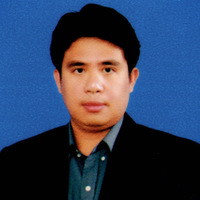
\includegraphics[width=2.8cm, height=2.8cm, keepaspectratio]{figures/chewa_official_portrait.jpg}};
        \end{scope}
    \end{tikzpicture}
\end{minipage}
\hfill
\begin{minipage}[c]{0.69\textwidth}
    {\fontsize{14}{18}\selectfont\bfseries\color{deepIndigo} ผู้ช่วยศาสตราจารย์ ดร.ชีวะ ทัศนา}\\[3pt]
    {\fontsize{10}{13}\selectfont\color{agriGreen}\textbf{ตำแหน่งทางวิชาการ: ผู้ช่วยศาสตราจารย์ สาขาวิชาฟิสิกส์}}\\[2pt]
    {\fontsize{9.5}{12}\selectfont คณะวิทยาศาสตร์และเทคโนโลยี มหาวิทยาลัยราชภัฏรำไพพรรณี}\\[2pt]
    {\fontsize{9}{11}\selectfont อีเมล: chewathassana@rbru.ac.th}
\end{minipage}

\vspace{8pt}
{\color{rbruBorder}\hrule height 0.8pt}
\vspace{8pt}

\noindent
\begin{minipage}[t]{0.48\textwidth}
    {\fontsize{11}{14}\selectfont\bfseries\color{deepIndigo} ประวัติการศึกษา}\\[4pt]
    {\fontsize{9}{12}\selectfont
    \begin{itemize}[leftmargin=1.2em, itemsep=2pt]
        \item \textbf{ปร.ด. (ฟิสิกส์ประยุกต์)}\\สถาบันเทคโนโลยีพระจอมเกล้า\\เจ้าคุณทหารลาดกระบัง
        \item \textbf{วท.ม. (ฟิสิกส์ประยุกต์)}\\สถาบันเทคโนโลยีพระจอมเกล้า\\เจ้าคุณทหารลาดกระบัง
        \item \textbf{วท.บ. ฟิสิกส์ (คอมพิวเตอร์และอิเล็กทรอนิกส์)}\\มหาวิทยาลัยนเรศวร
    \end{itemize}}
\end{minipage}
\hfill
\begin{minipage}[t]{0.48\textwidth}
    {\fontsize{11}{14}\selectfont\bfseries\color{deepIndigo} ความเชี่ยวชาญและงานวิจัย}\\[4pt]
    {\fontsize{9}{12}\selectfont
    \begin{itemize}[leftmargin=1.2em, itemsep=2pt]
        \item ฟิสิกส์เกษตรดิจิทัลและไอโอที\\(AIoT SmartFarm)
        \item ปัญญาประดิษฐ์และการเรียนรู้เชิงลึก\\(Computer Vision)
        \item การคำนวณโครงสร้างสารแม่เหล็ก\\และควอนตัมฟิสิกส์
    \end{itemize}}
\end{minipage}

\end{document}
